\documentclass{article}
\usepackage[margin=2cm]{geometry}
\usepackage[ngerman]{babel}
\usepackage{float}
\usepackage{graphicx}
\usepackage{comment}
\usepackage[version=4]{mhchem}
\usepackage{siunitx}
\usepackage{hyperref}

\title{OC2 Reaktionen}
\author{}
\date{\today}

\begin{document}

\maketitle
\tableofcontents
\newpage

\section{Aldehyde und Ketone}
\subsection{wichtige Vertreter}
\subsection{Technische Synthese Formaldehyd}
\begin{figure}[H]
	\centering
	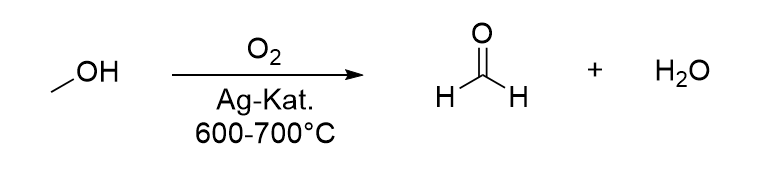
\includegraphics[width=0.75\linewidth]{Bilder/technische Synthese Formaldehyd.png}
\end{figure}

\subsection{Technische Synthese Acetaldehyd}
\begin{figure}[H]
	\centering
	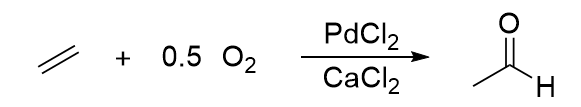
\includegraphics[width=0.65\linewidth]{Bilder/technische Synthese Acetaldehyd.png}
\end{figure}

\subsection{Elektrophile Additionen}
\subsubsection{Protonierung von Carbonylen}
\begin{figure}[H]
	\centering
	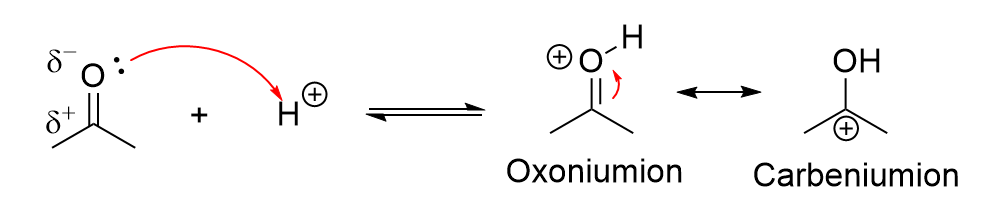
\includegraphics[width=0.8\linewidth]{Bilder/Protonierung-von-Carbonylen.png}
\end{figure}

\subsubsection{Oligomerisierung/Polymerisation}
\begin{figure}[H]
	\centering
	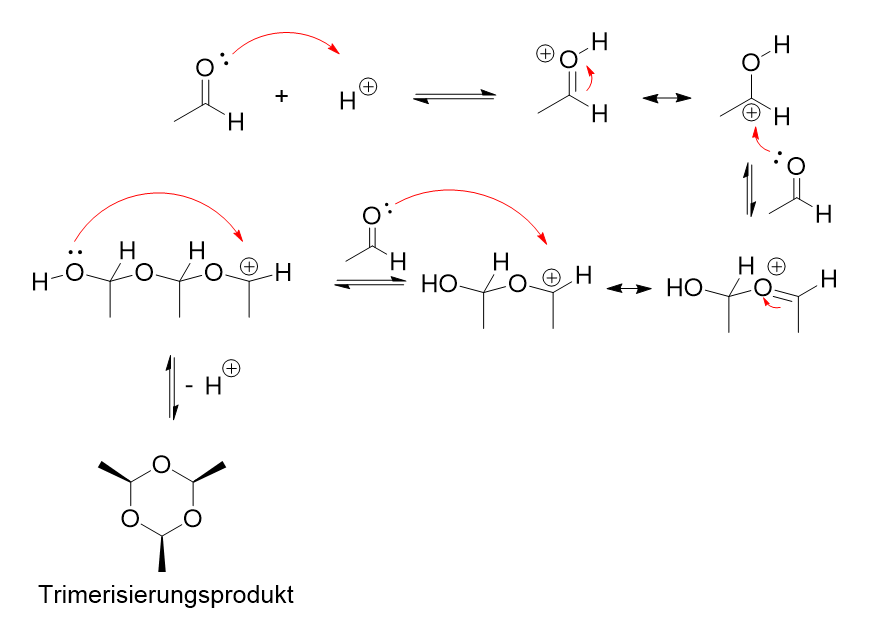
\includegraphics[width=0.9\linewidth]{Bilder/trimerisierung von Acetaldehyd.png}
\end{figure}
\subsubsection*{Polymerisierung von Formaldehyd}
\begin{figure}[H]
	\centering
	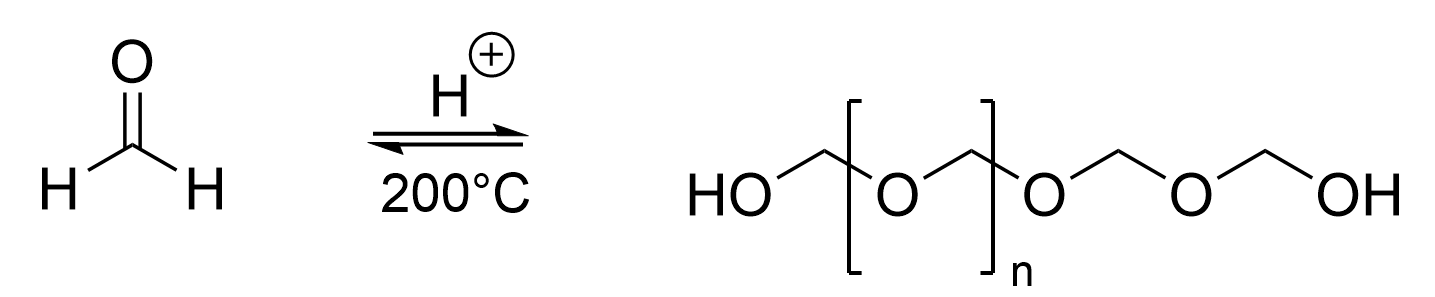
\includegraphics[width=0.65\linewidth]{Bilder/polymerisierung Formaldehyd.png}
\end{figure}

\subsection{Nucleophile Additionen}
\begin{figure}[H]
	\centering
	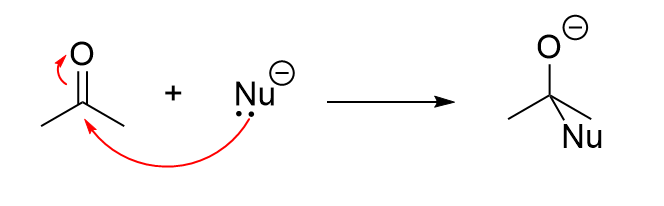
\includegraphics[width=0.6\linewidth]{Bilder/Nucleophile Addition an Carbonylen.png}
\end{figure}
\noindent Häufig ist der nucleophilen Substitution eine Aktivierung der Carbonylgruppe vorgelagert.
\begin{figure}[H]
	\centering
	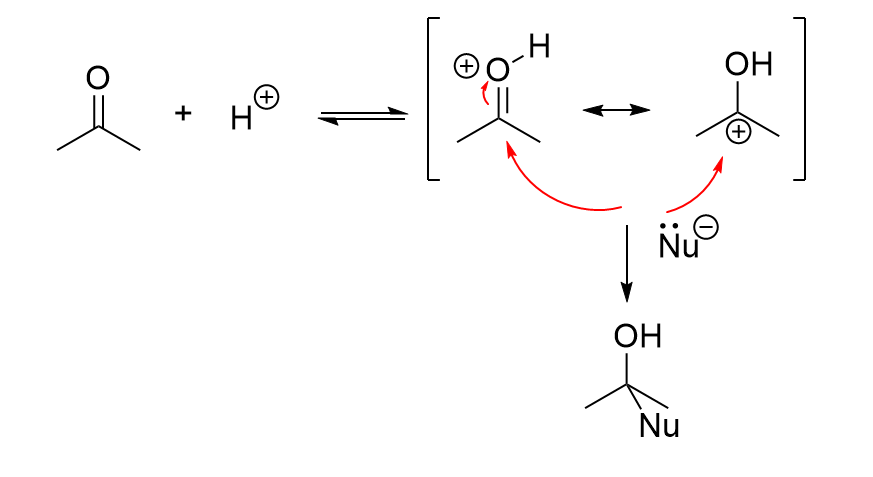
\includegraphics[width=0.8\linewidth]{Bilder/Nucleophile-addition-mit-aktivierung.png}
\end{figure}
\subsubsection{Hydrate}
\begin{figure}[H]
	\centering
	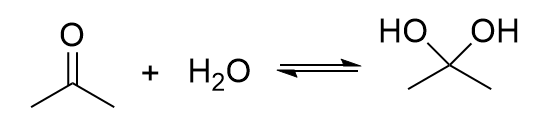
\includegraphics[width=0.5\linewidth]{Bilder/hydrate.png}
\end{figure}
Die Hinreaktion ist begünstigt wenn kein sterisch gehindertes Molekül hydriert wird.
Elektronenziehende Substituenten vorhanden sind. Die Rückreaktion ist begünstigt bei 
elektronenschiebenden Substituenten.
\subsubsection{Bisulfit-Addukte}
\begin{figure}[H]
	\centering
	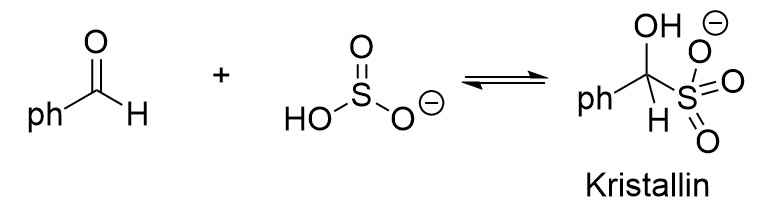
\includegraphics[width=0.7\linewidth]{Bilder/bisulfit-addukte.png}
\end{figure}
Die Bisulfit-Addukte wurden in der Vergangenheit als Nachweis verwendet, da die kristallinen Feststoffe Aussagen über das zu analysierende Edukt der Reaktion geben.

\subsubsection{Halbacetale/Acetale}
\begin{figure}[H]
	\centering
	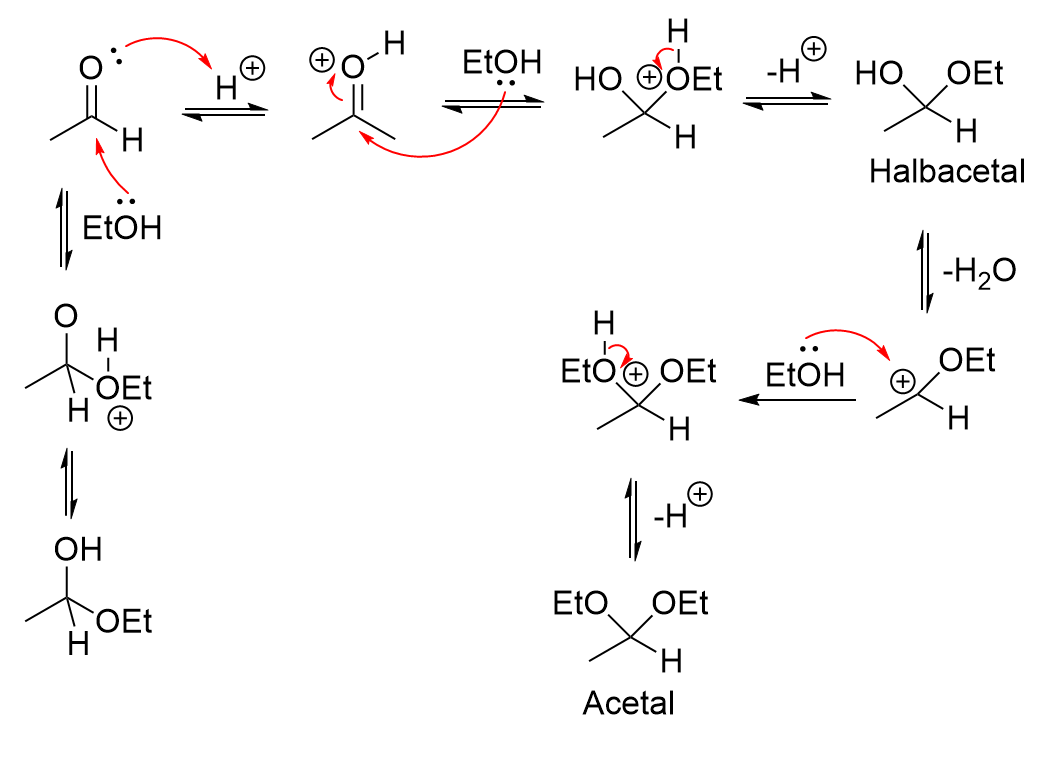
\includegraphics[width=0.9\linewidth]{Bilder/Halbacetale und acetale.png}
\end{figure}
Die Reaktion wird von Säuren katalysiert, sie beeinflussen nicht das Gleichgewicht.
Unter Wasserentziehenden Bedingungen ist die Acetalbildung begünstigt.

\subsubsection*{Cyclische Halbacetale}
\subsubsection{Halbacetale/Acetale}
\begin{figure}[H]
	\centering
	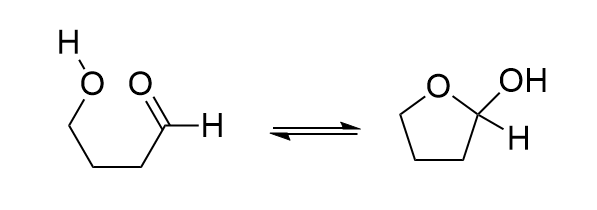
\includegraphics[width=0.55\linewidth]{Bilder/cyclische Acetale.png}
\end{figure}

\subsubsection*{Acetalspaltung}
\begin{figure}[H]
	\centering
	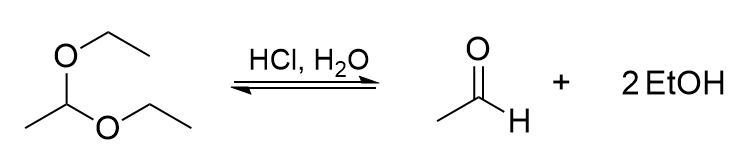
\includegraphics[width=0.6\linewidth]{Bilder/Acetalspaltung.png}
\end{figure}

\subsubsection*{Acetale als Schutzgruppen}
Acetale, besonders cyclische Acetale können als Schutzgruppe für Carbonsäuren dienen.
Cyclische Acetale sind stabiler als acyclische, da die Entropieänderung $\Delta S=0$ ist, während sie bei acyclischen Acetalen $\Delta S<0$ ist.
\begin{figure}[H]
	\centering
	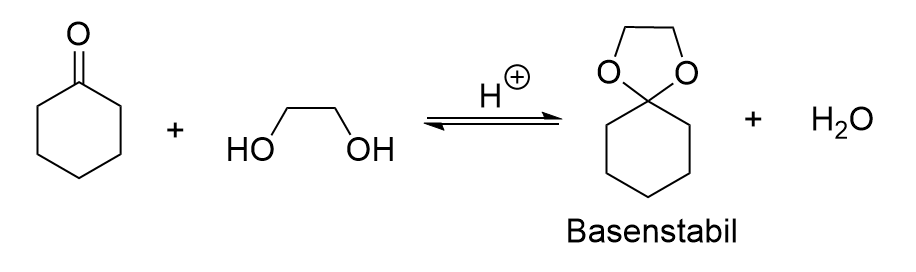
\includegraphics[width=0.7\linewidth]{Bilder/acetalschutzgruppen.png}
\end{figure}

\subsubsection*{Dithioacetale}
\begin{figure}[H]
	\centering
	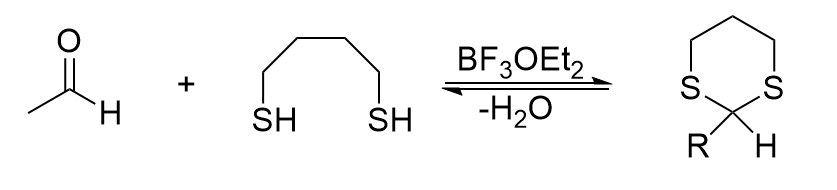
\includegraphics[width=0.65\linewidth]{Bilder/Dithioacetale.png}
\end{figure}
Der Mechanismus ist analog zur Acetalisierung mit Saurerstoffen. 
Dithioacetale finden Anwendung in der Corey-Seebach-Umpolung
\subsubsection*{Corey-Seebach-Umpolung}
\begin{figure}[H]
	\centering
	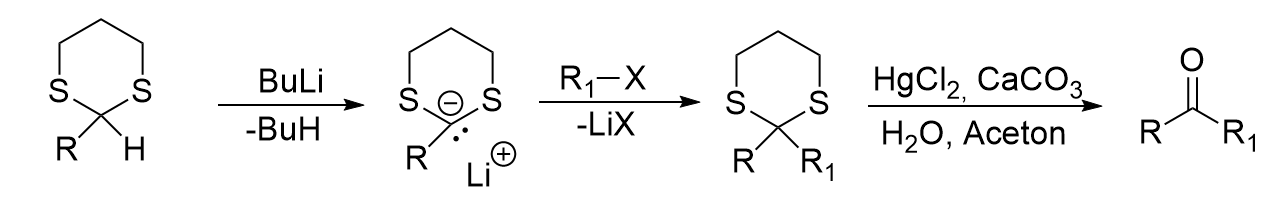
\includegraphics[width=0.95\linewidth]{Bilder/corey-seebach-umpolung.png}
\end{figure}
Würde hier anstelle des Schwefels ein Sauerstoff sitzen, würde die REaktion nicht
stattfinden. Schwefel ist weniger elektronegativ und größer. Das Carbenium-Ion wird durch die 
d-Orbitale am Schwefel stablisiert. 
\subsubsection{N,N-Acetale}
\begin{figure}[H]
	\centering
	\includegraphics[width=0.8\linewidth]{Bilder/NN-Acetale.png}
\end{figure}

\subsubsection{Imine, Oxime, Hydrazone, Semicarbazone}
\begin{figure}[H]
	\centering
	\includegraphics[width=0.8\linewidth]{Bilder/imin.png}
\end{figure}
Die optimale Reaktionsgeschwindigkeit ist beim $pK_s$ des Amins.
Säureaktivierung der Carbonylverbindung beschleunigt die Reaktion, zuviel Säure ist kontraproduktiv,
da das Amin vollständig protoniert wäre und damit nicht mehr nucleophil wäre.\\

\noindent Für alle anderen Stoffklassen gilt der Mechanismus analog.
\begin{figure}[H]
	\centering
	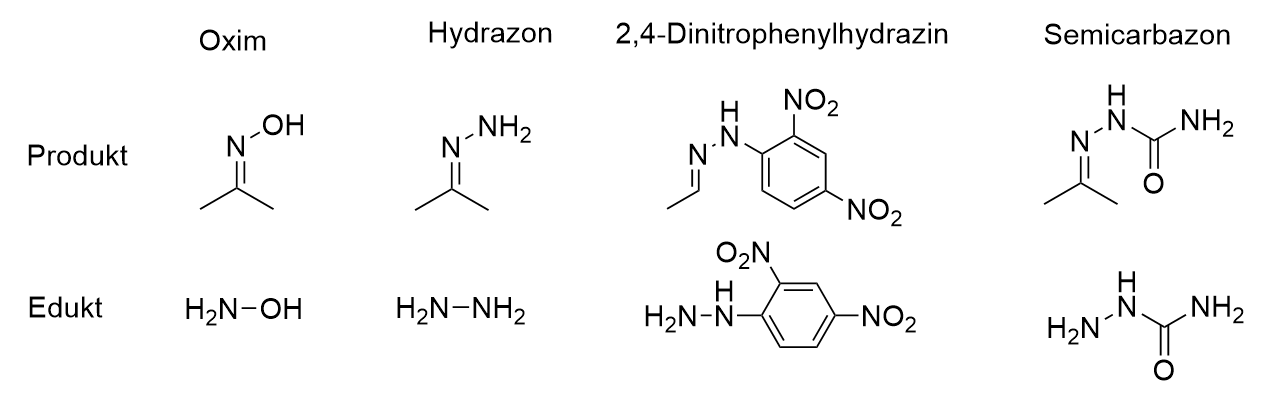
\includegraphics[width=1\linewidth]{Bilder/imin-oxim-hydrazon-semicarbazon.png}
\end{figure}


\subsubsection{sekundäre Amine und Ketone mit $\alpha$-H-Atom}
Sekundäre Amine und Ketone mit $\alpha$-H-Atom reagieren zu Enaminen.
\begin{figure}[H]
	\centering
	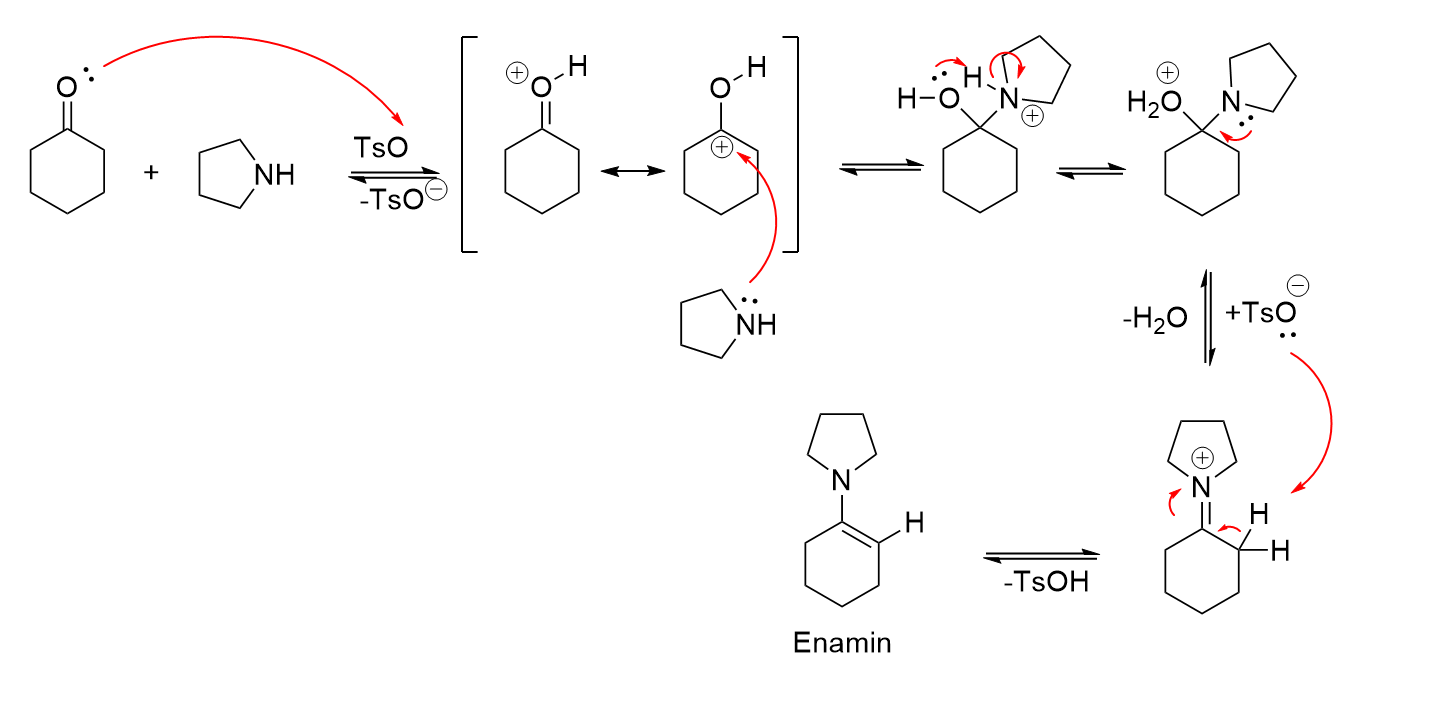
\includegraphics[width=1.1\linewidth]{Bilder/enamine.png}
\end{figure}


\subsubsection{Cyanhydrine}
\begin{figure}[H]
	\centering
	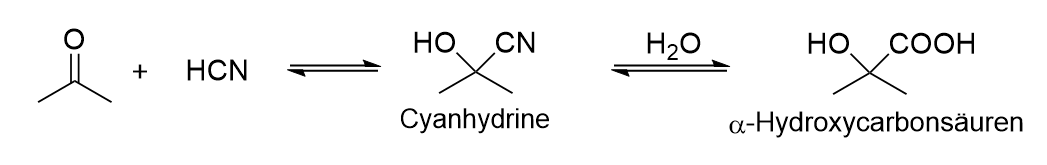
\includegraphics[width=0.8\linewidth]{Bilder/Cyanhydrine.png}
\end{figure}

\subsubsection{Alkohole durch Grignard-Addition}
\begin{figure}[H]
	\centering
	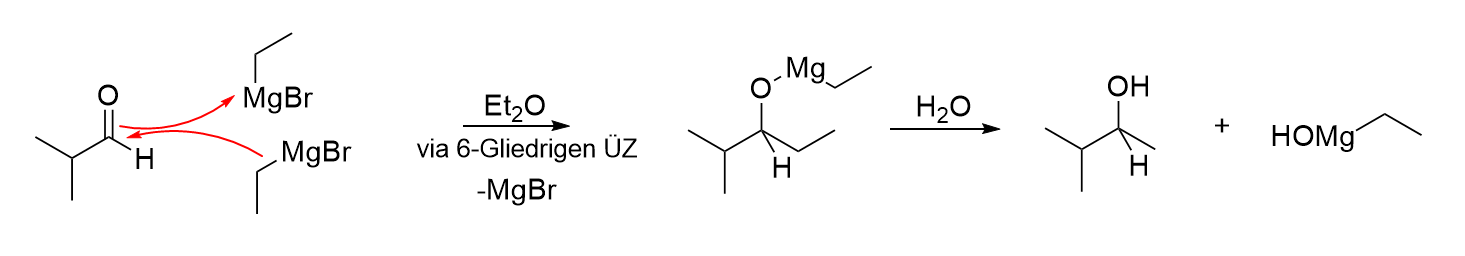
\includegraphics[width=1.1\linewidth]{Bilder/Grignard zu Alkoholen.png}
\end{figure}


\subsubsection*{Übersicht Grignard}
\begin{figure}[H]
	\centering
	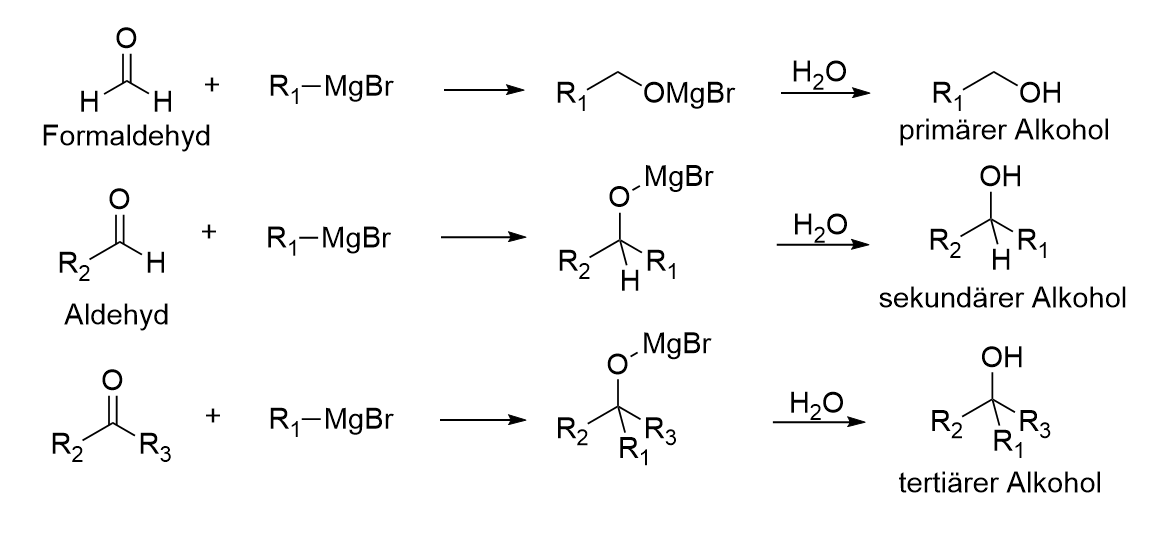
\includegraphics[width=0.9\linewidth]{Bilder/Grignard Übersicht.png}
\end{figure}


\subsubsection{Benzoinkondensation}
\begin{figure}[H]
	\centering
	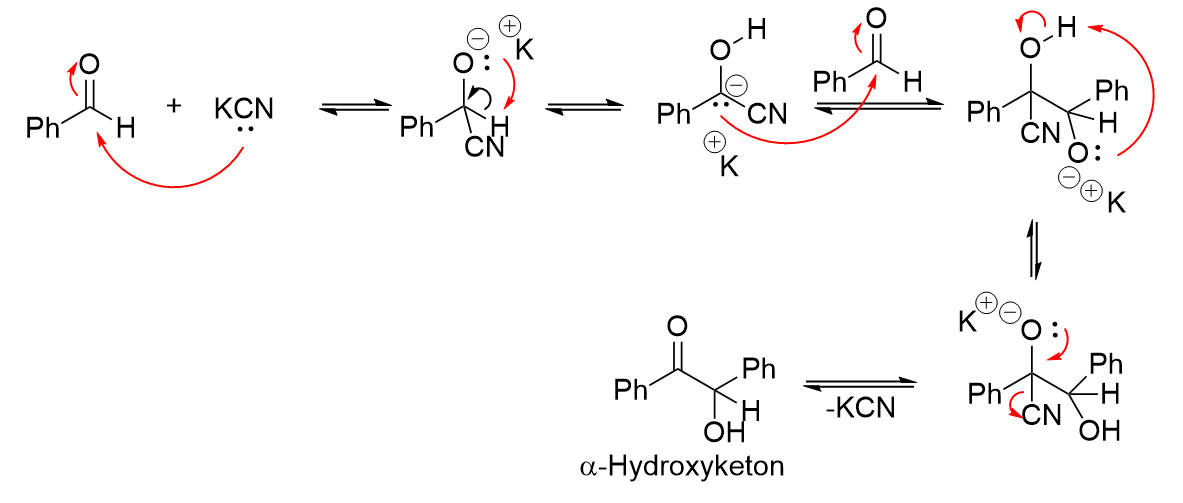
\includegraphics[width=0.9\linewidth]{Bilder/Benzoinkondensation.png}
\end{figure}

\subsubsection{Stetter Reaktion}
\begin{figure}[H]
	\centering
	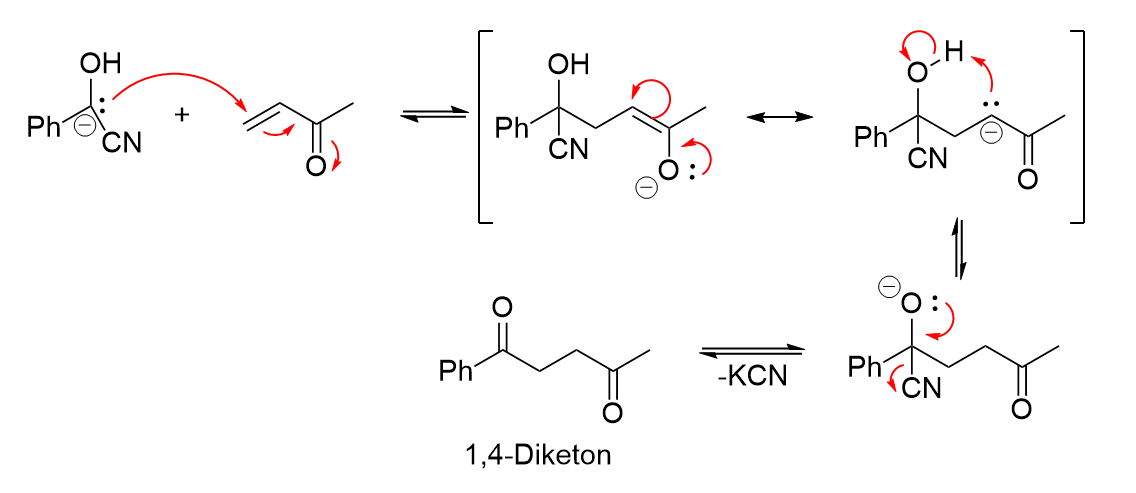
\includegraphics[width=0.9\linewidth]{Bilder/Stetter Reaktion.png}
\end{figure}
Als Alternative zu Cyanid können Thiazoliumsalze als Katalysatoren verwendet werden.
\begin{figure}[H]
	\centering
	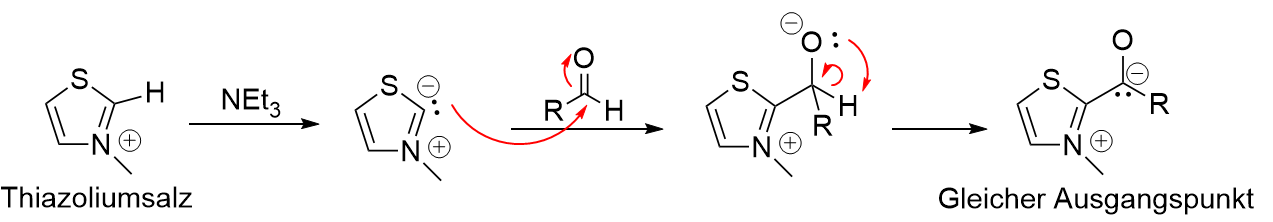
\includegraphics[width=1\linewidth]{Bilder/Stetter mit Thiazoliumsalzen.png}
\end{figure}

\subsubsection{Aminotriphenylmethanfarbstoffe}
\begin{figure}[H]
	\centering
	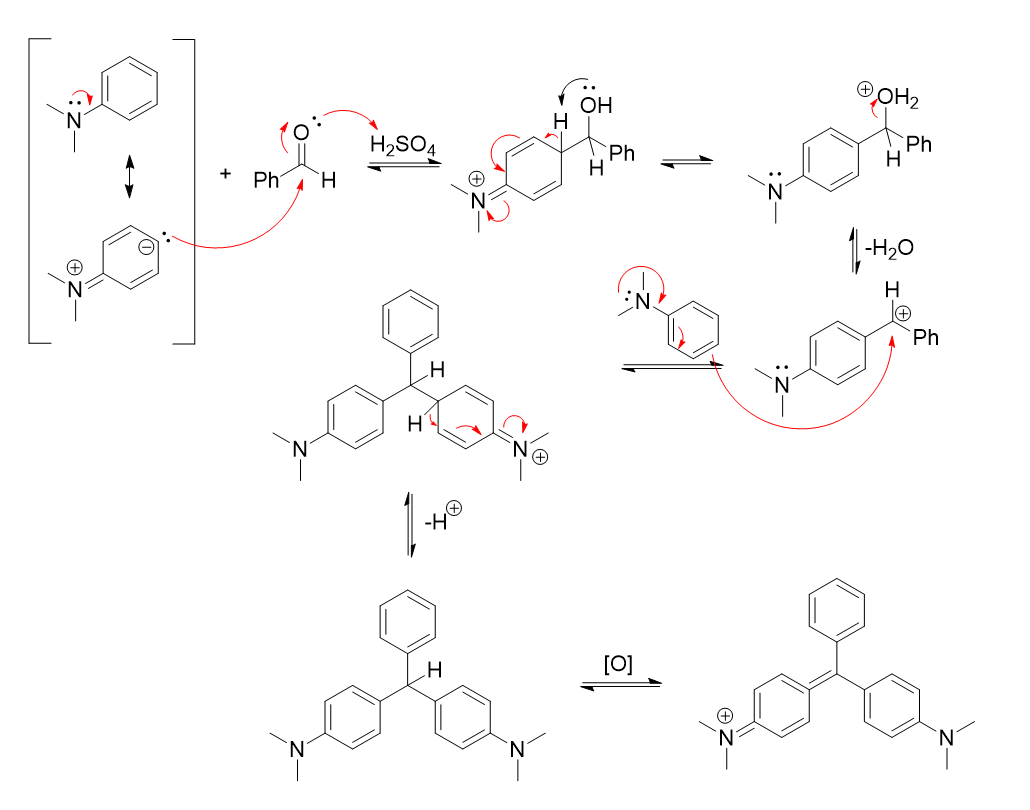
\includegraphics[width=1\linewidth]{Bilder/Aminotriphenylmethanfarbstoffe.png}
\end{figure}
Oxidationsmittel für den letzten Reaktionsschritt können Bleioxid, Schwefelsäure oder schon Luftsauerstoff sein.
Auxochrome Gruppen wie \ce{NH2}, \ce{NHR}, \ce{NR2}, \ce{OH}, \ce{OMe} üben einen -M-Effekt auf die Triphenylmethanfarbstoffe aus und verstärken dadurch die Farbe.
Ein Farbiger Stoff der chromophore Gruppen enthält (Gruppen weshalb er Farbig ist) ist nicht direkt ein Farbstoff. 
Erst durch die Einführung auxochromer Gruppen wird eine Farbige Verbindung zum Farbstoff.


\subsubsection{Wittig Reaktion}
\subsubsection*{Reaktionsgleichung}
\begin{figure}[H]
	\centering
	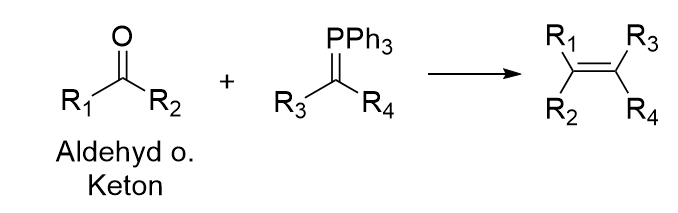
\includegraphics[width=0.57\linewidth]{Bilder/Wittig Reaktion RG.png}
\end{figure}

\subsubsection*{Reaktionsmechanismus}
\begin{figure}[H]
	\centering
	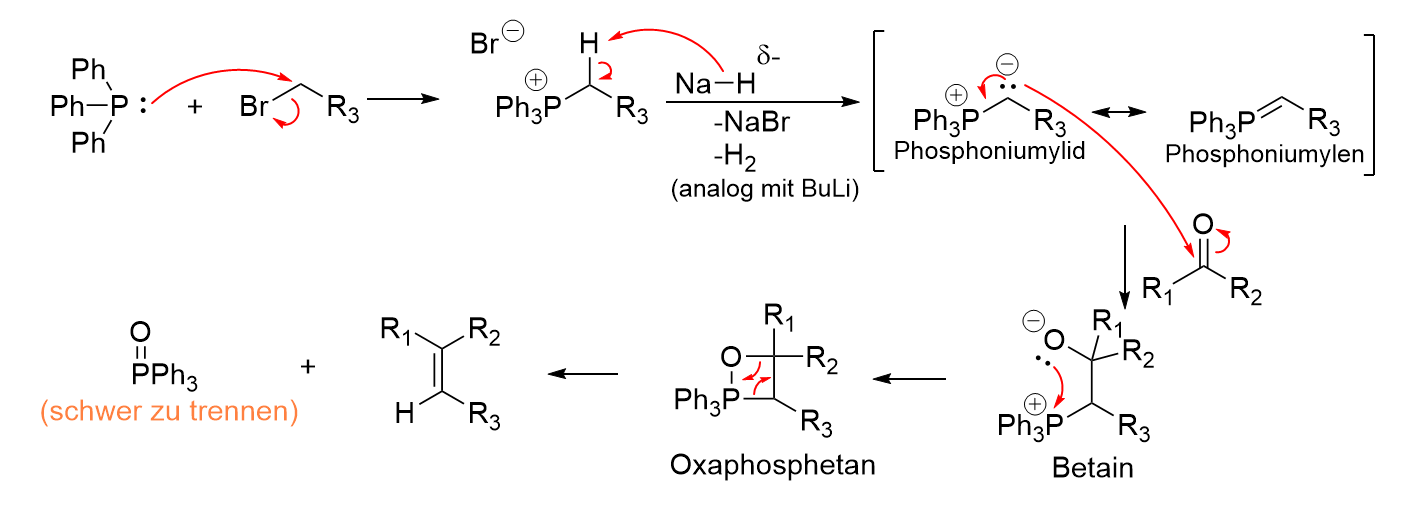
\includegraphics[width=1.1\linewidth]{Bilder/Wittig.png}
\end{figure}

%E/Z Selektivität fehlt
Die Phosphoniumylide weisen unterschiedliche Stabilitäten auf. Dies sind nachfolgend aufgeführt.
\begin{figure}[H]
	\centering
	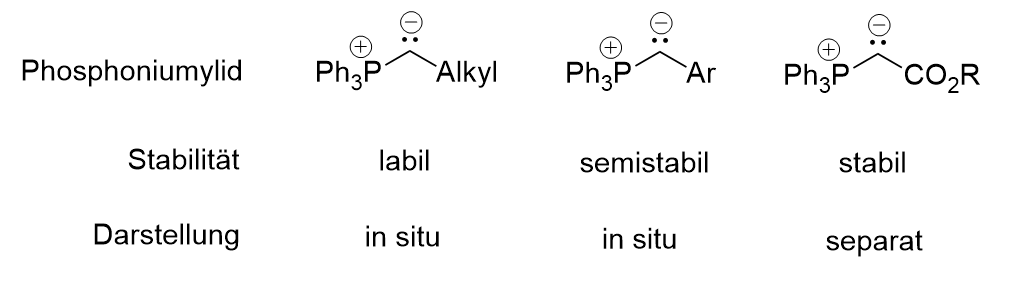
\includegraphics[width=0.8\linewidth]{Bilder/Phosphoniumylid Übersicht.png}
\end{figure}
\noindent Die Darstellung der Phosphoniumylide mit verschiedenen Reagenzien führt zu unterschiedlichen Stereoselektivitäten.
\begin{table}[H]
	\centering
	\begin{tabular}{|c|c|c|c|}
		\hline
		\textbf{Reagenzien}&n-BuLi&NaOEt&NaOH\\
		&\ce{KO^tBu}&\ce{NaOH_{(aq)}}&\\
		&\ce{NaNH2}&&\\
		&\ce{Na^+ ^-CH2SOCH3}&&\\
		\hline
		\textbf{Stereoselektivität}&$\ge 90$\% Z-Isomer&Z/E-Gemisch&$>$90\%E\\
		\hline
	\end{tabular}
\end{table}

\subsubsection{Horner-Wadsworth-Emmons-Reaktion}
\begin{figure}[H]
	\centering
	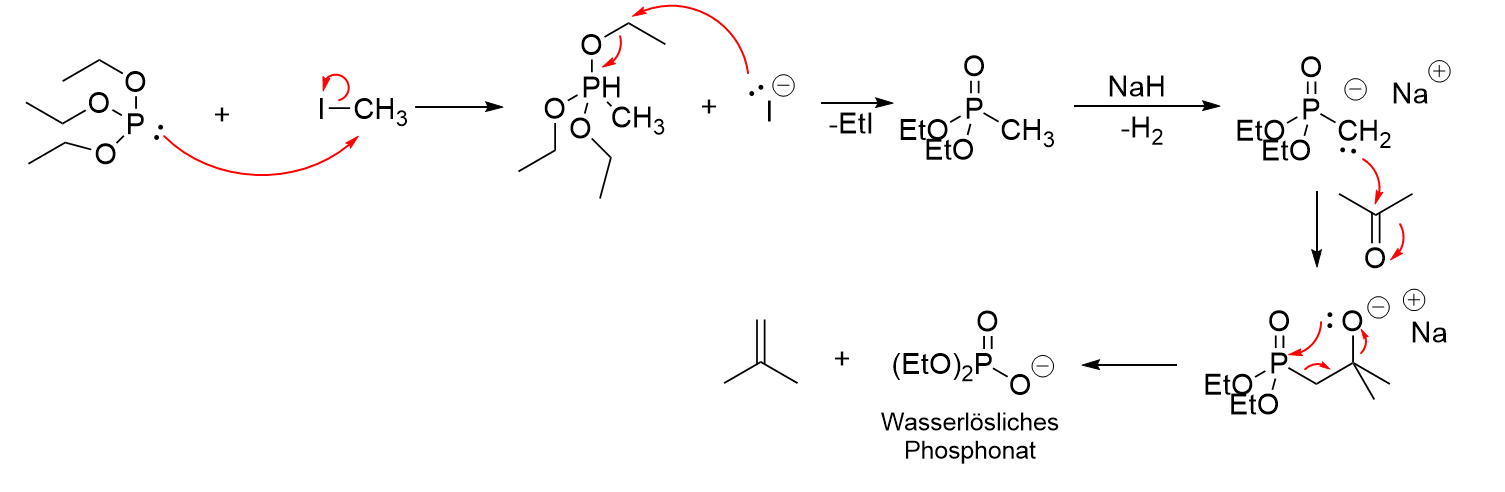
\includegraphics[width=1\linewidth]{Bilder/HWE-Reaktion.png}
\end{figure}
Das Wasserlösliche Phosphonat ermöglicht eine leichere Abtrennung im Vergleich zur Wittig-Reaktion.
Der Nachteil der HWE Reaktion ist, dass das Phosphonat im Abwasser nicht durch Mikroorganismen abgebaut. 

%\subsubsection{Schwefelhaltige Ylide}
%Ich weiß nicht was genau man zu Schwefelyliden aufschreiben soll.

\subsection{Oxidationen und Reduktionen}
\subsubsection{Oxidation von Aldehyden}
\begin{figure}[H]
	\centering
	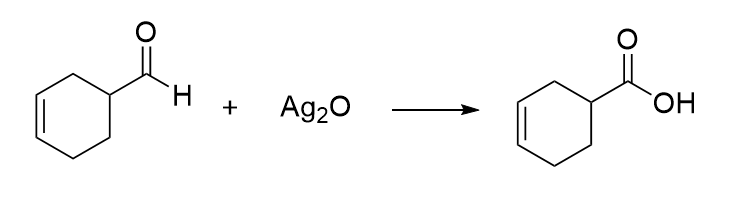
\includegraphics[width=0.6\linewidth]{Bilder/chemoselektive oxidation von aldehyden.png}
\end{figure}
Diese Oxidation ist eine chemoselektive oxidation gegenüber Doppelbindungen. Dies bedeutet es wird in einem Molekül nur eine bestimmte Gruppe, in diesem Fall der Aldehyd, umgesetzt, andere bleiben unberührt.
Als Oxidationsmittel eignen sich: \ce{CrO3}, \ce{Ag2O}, \ce{H2O2}, \ce{KMnO4} und Persäuren.

\subsubsection{Oxidation von Benzaldehyd zur Perbenzoesäure}
\begin{figure}[H]
	\centering
	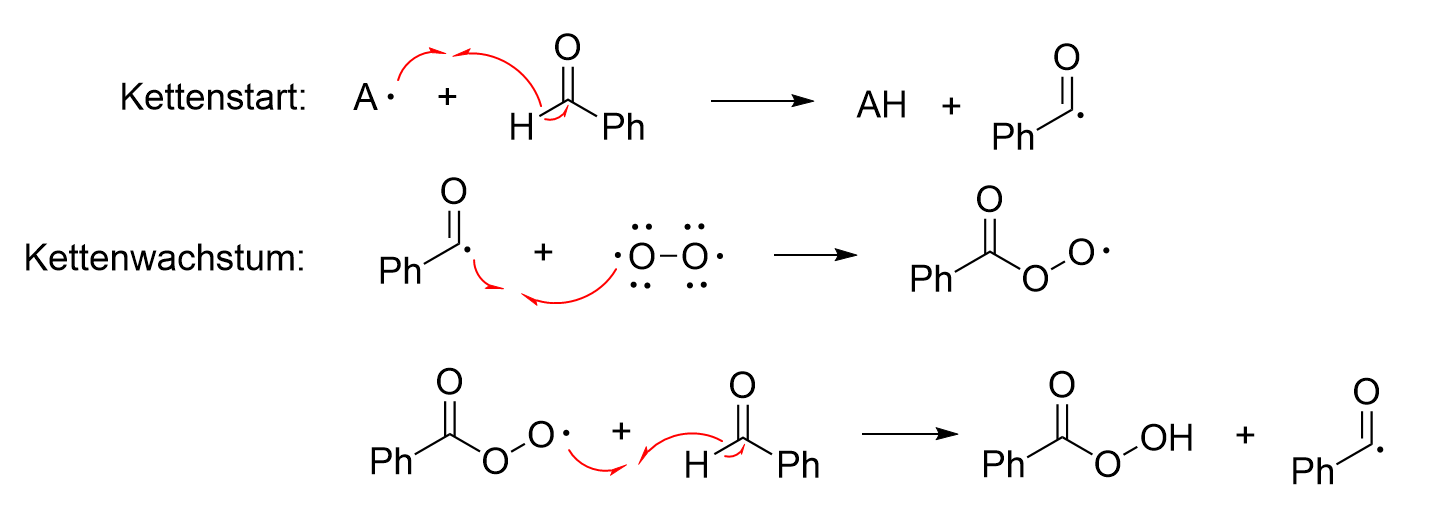
\includegraphics[width=0.9\linewidth]{Bilder/Oxidation von benzaldehyd.png}
\end{figure}
Der Kettenabbruch ist analog zur Radikalischen Substitution.


\subsubsection{Baeyer-Villiger-Oxidation}
\subsubsection*{Reaktionsgleichung}
\begin{figure}[H]
	\centering
	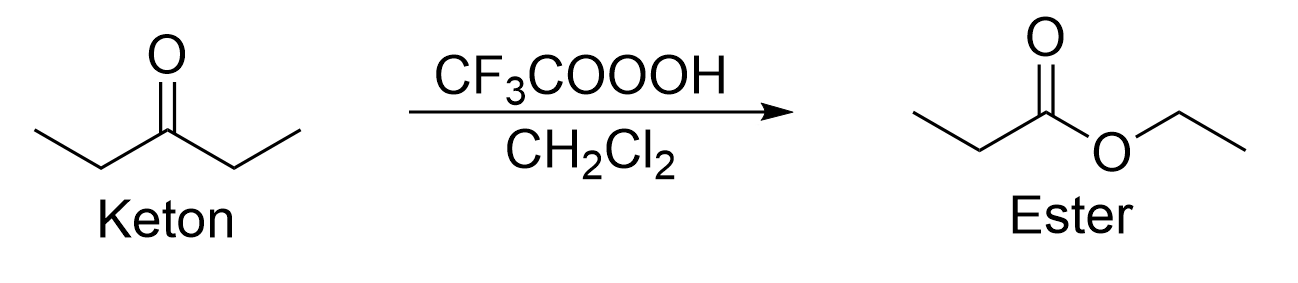
\includegraphics[width=0.65\linewidth]{Bilder/Bayer-Villiger-Oxidation-RG.png}
\end{figure}
Cyclische Ketone reagieren analog und bilden ein Lacton.
\subsubsection*{Mechanismus}
\begin{figure}[H]
	\centering
	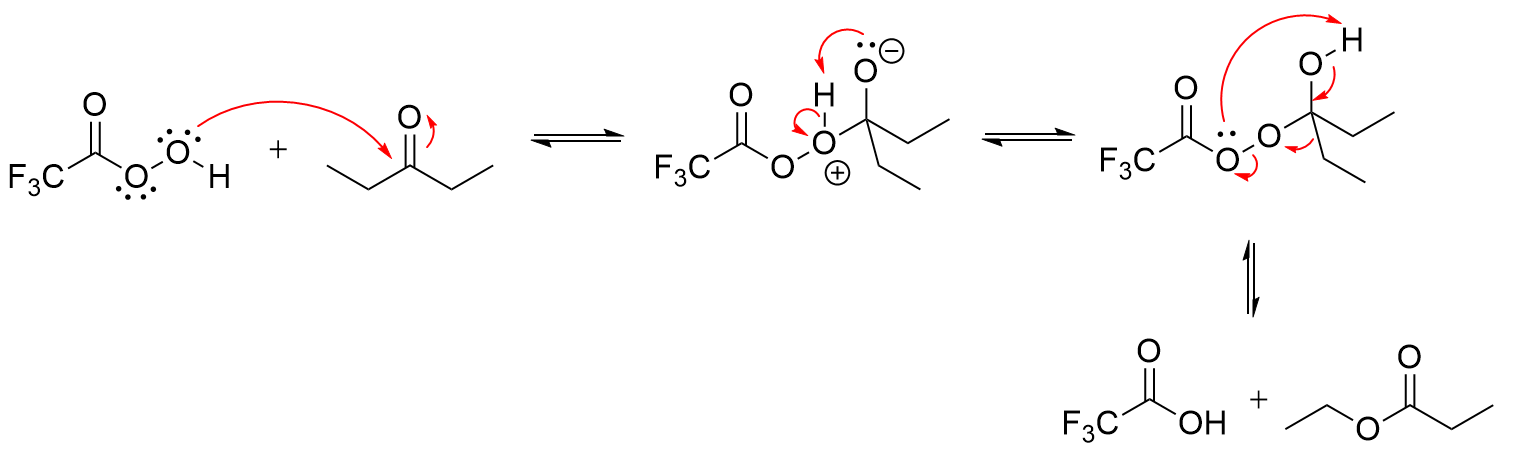
\includegraphics[width=1.1\linewidth]{Bilder/Bayer-Villiger-oxidation-Mechanismus.png}
\end{figure}
Handelt es sich um ein unsymmetrisches Keton, so gibt es folgende Wanderungstendenzen von Resten am ursprünglichen Carbonyl-Kohlenstoff zum Sauerstoff.
\begin{equation*}
	\ce{H} > \ce{tert-Alkyl} > \ce{sek-Alkyl} > \ce{Ph} > \ce{prim-Alkyl} > \ce{Me}
\end{equation*}

%\subsubsection{Spezialfall der Baeyer-Villiger-Oxidation}
%scheint unnötig

\subsubsection{Clemmensen-Reduktion}
\begin{figure}[H]
	\centering
	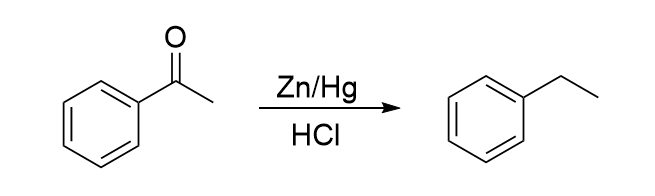
\includegraphics[width=0.6\linewidth]{Bilder/clemmensen-Reduktion.png}
\end{figure}

\subsubsection{Katalytische Hydrierung}
\begin{figure}[H]
	\centering
	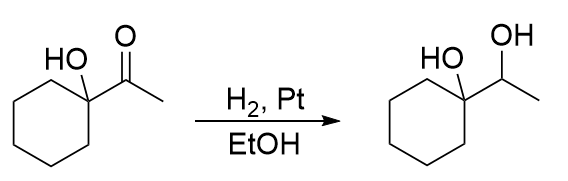
\includegraphics[width=0.5\linewidth]{Bilder/Katalytische Hydrierung mit Pt.png}
\end{figure}


\begin{figure}[H]
	\centering
	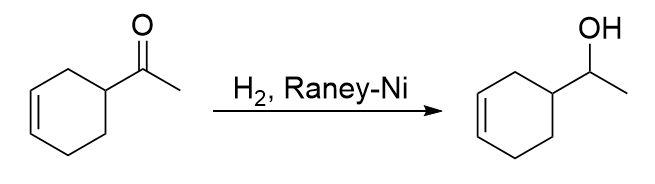
\includegraphics[width=0.55\linewidth]{Bilder/katalytische Hydrierung Raney.png}
\end{figure}
Die Katalytische Hydrierung mit Raney-Nickel ist chemoselektiv und hydriert keine Doppelbindungen. Für die Hydrierung mit Platin gilt dies nicht. 

\subsubsection{Wolf-Kishner-Reduktion}
\subsubsection*{Reaktionsgleichung}
\begin{figure}[H]
	\centering
	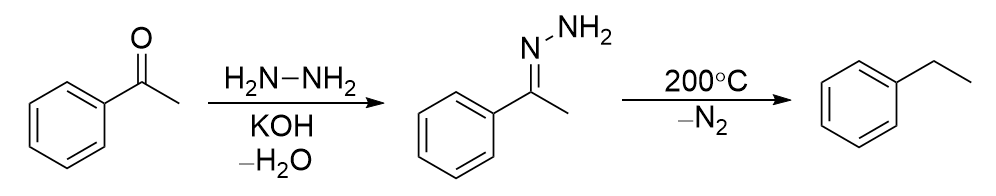
\includegraphics[width=0.8\linewidth]{Bilder/Wolff-kishner-Reduktion.png}
\end{figure}
Dies ist eine Alternative wenn man die Clemmensen Reduktion mit Quecksilber umgehen will.
\subsubsection*{Mechanismus}
Nachfolgend ist der Mechanismus ab dem Hydrazon gezeigt.
\begin{figure}[H]
	\centering
	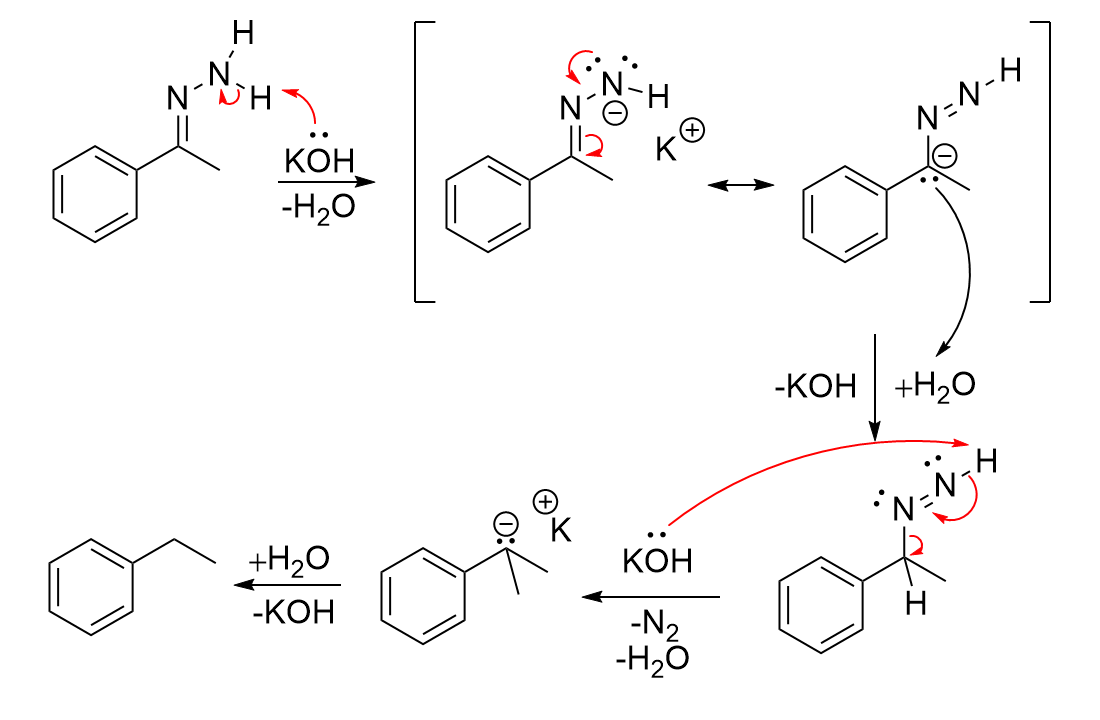
\includegraphics[width=0.8\linewidth]{Bilder/wolff-kishner-Mechanismus.png}
\end{figure}


\subsubsection{Reduktion mit Metallhydriden}
\begin{figure}[H]
	\centering
	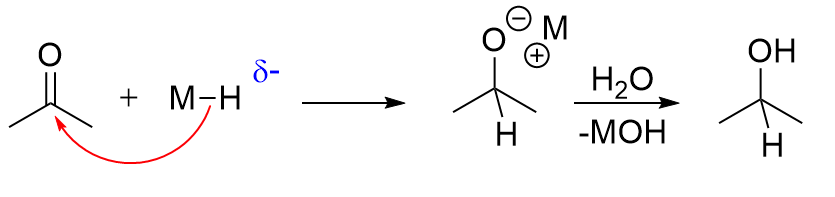
\includegraphics[width=0.7\linewidth]{Bilder/Reduktion mit Metallhydriden.png}
\end{figure}
\ce{LiAlH4} reagiert heftig mit protischen Lösemitteln daher müssen bei Verwendung des 
Reduktionsmittels stehts aprotische Lösemittel wie THF oder Diethylether verwendet werden. 
\ce{NaBH4} hingegen hat eine größere Stabilität in protischen Lösemitteln und kann daher auch verwendet werden sofern sich die zu reduzierende Substanz 
nicht in aprotischen Lösemitteln löst. 
\subsubsection{Meerwein Ponndorf Verley Reduktion / Oppenheimer Oxidation}
\begin{figure}[H]
	\centering
	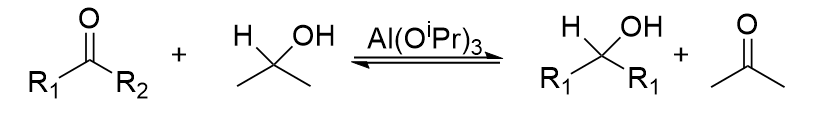
\includegraphics[width=0.8\linewidth]{Bilder/Meerwein-Ponndorf-Verley.png}
\end{figure}

\subsubsection*{Mechanismus}
\begin{figure}[H]
	\centering
	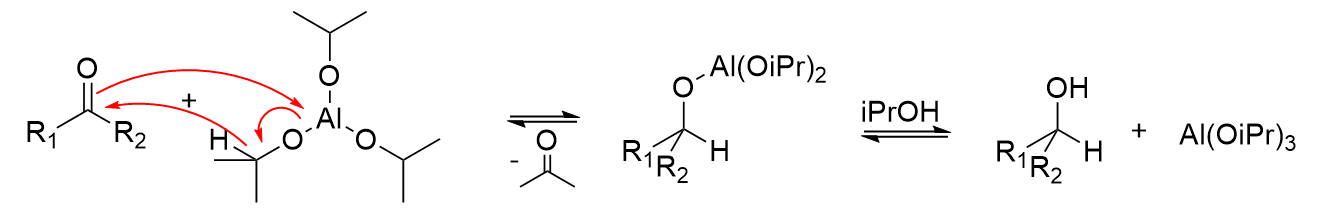
\includegraphics[width=1\linewidth]{Bilder/Meerwein-pondorf-Verley-Mechanismus.png}
\end{figure}

\subsubsection{Cannizzaro-Reaktion}
\subsubsection*{Bilanzgleichung}
\begin{figure}[H]
	\centering
	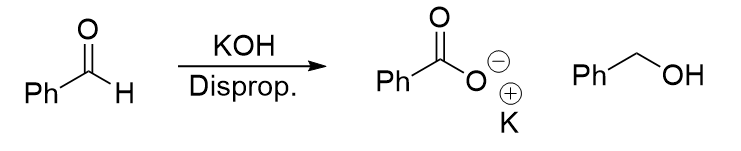
\includegraphics[width=0.65\linewidth]{Bilder/Cannizzaro-Bilanzgleichung.png}
\end{figure}
\subsubsection*{Mechanismus}
\begin{figure}[H]
	\centering
	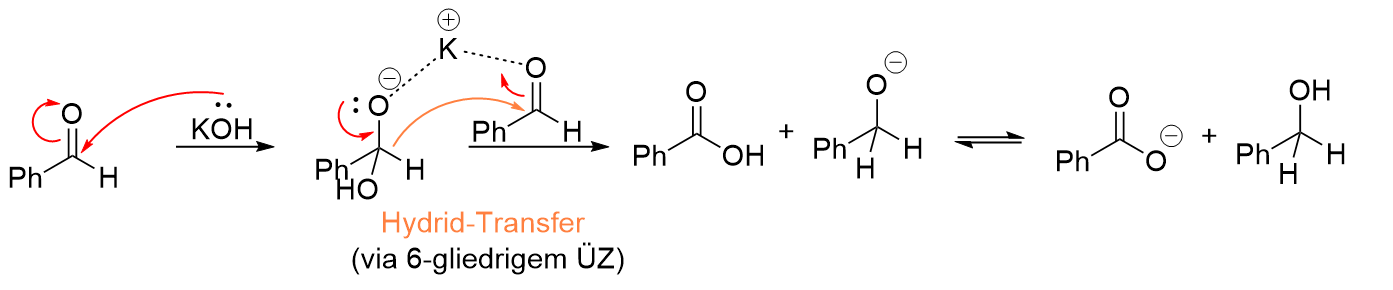
\includegraphics[width=1.1\linewidth]{Bilder/Cannizzaro-Mechanismus.png}
\end{figure}
\subsubsection*{Gekreuzte Cannizzaro-Reaktion mit Formaldehyd}
\begin{figure}[H]
	\centering
	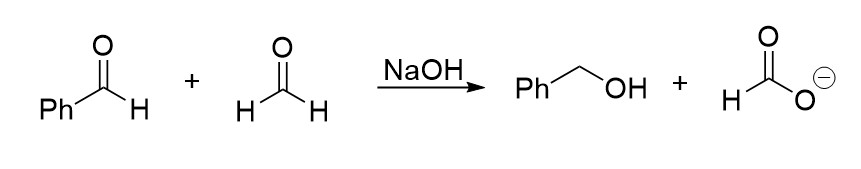
\includegraphics[width=0.75\linewidth]{Bilder/Gekreuzte Cannizzaro.png}
\end{figure}

\subsubsection{Leuchat-Wallach-Reaktion}
Anderer Name: \textbf{Reduktive Aminierung von Ketonen/Aldehyden}
\subsubsection*{Bilanzgleichung}
\begin{figure}[H]
	\centering
	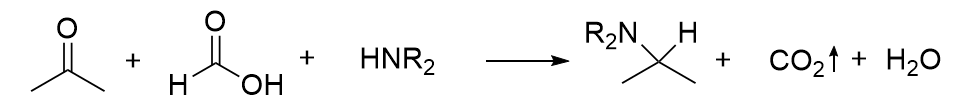
\includegraphics[width=0.75\linewidth]{Bilder/Leuchat-Wallach-Reaktion.png}
\end{figure}

\subsubsection*{Mechanismus}
\begin{figure}[H]
	\centering
	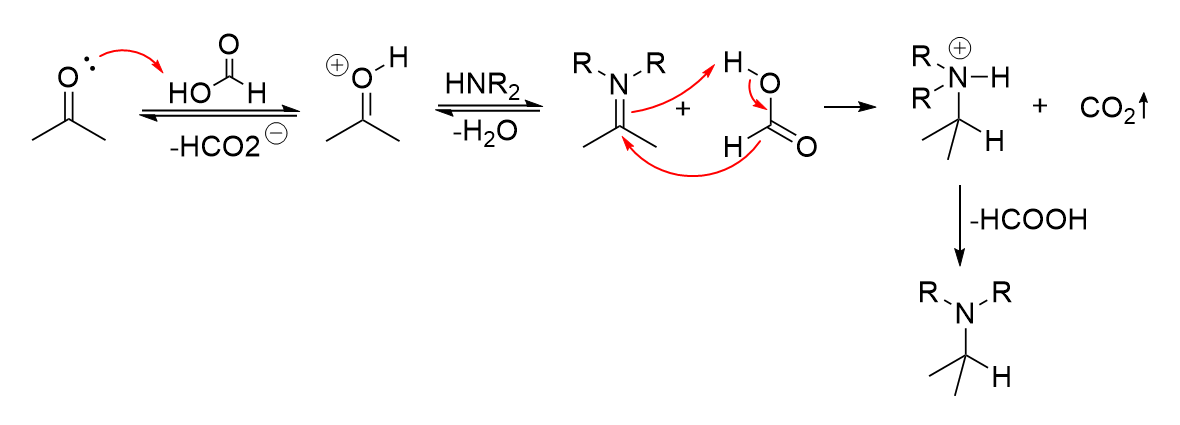
\includegraphics[width=0.9\linewidth]{Bilder/Leuchat Wallach Reaktion Mechanismus.png}
\end{figure}

\subsubsection{Einelelktronenreduktion}
\subsubsection*{Pinakolkupplung}
\begin{figure}[H]
	\centering
	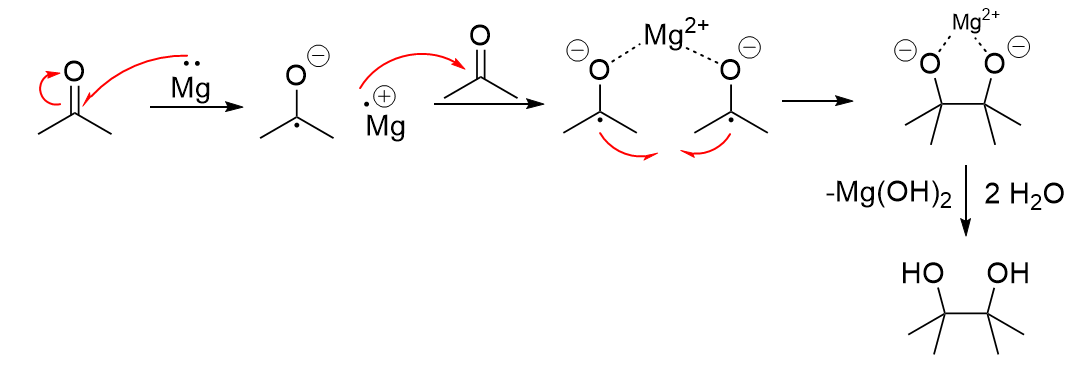
\includegraphics[width=0.9\linewidth]{Bilder/Pinakolkupplung.png}
\end{figure}


\subsubsection{Enzymatische Reduktion}
\begin{figure}[H]
	\centering
	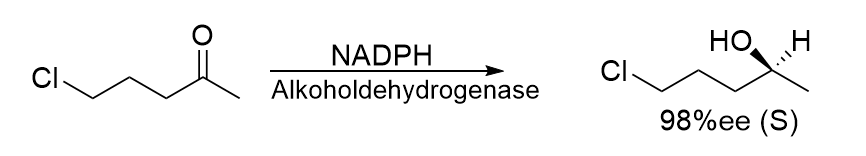
\includegraphics[width=0.8\linewidth]{Bilder/Enzymatische Reduktion.png}
\end{figure}
Die Reaktion ist chemoselektiv (reduziert in diesem Beispiel nur das Keton und nicht das Chlor) und enantioselektiv.


\subsection{Reaktionen von Enolen und Enolaten}
\subsubsection{Allgemeines}
\begin{figure}[H]
	\centering
	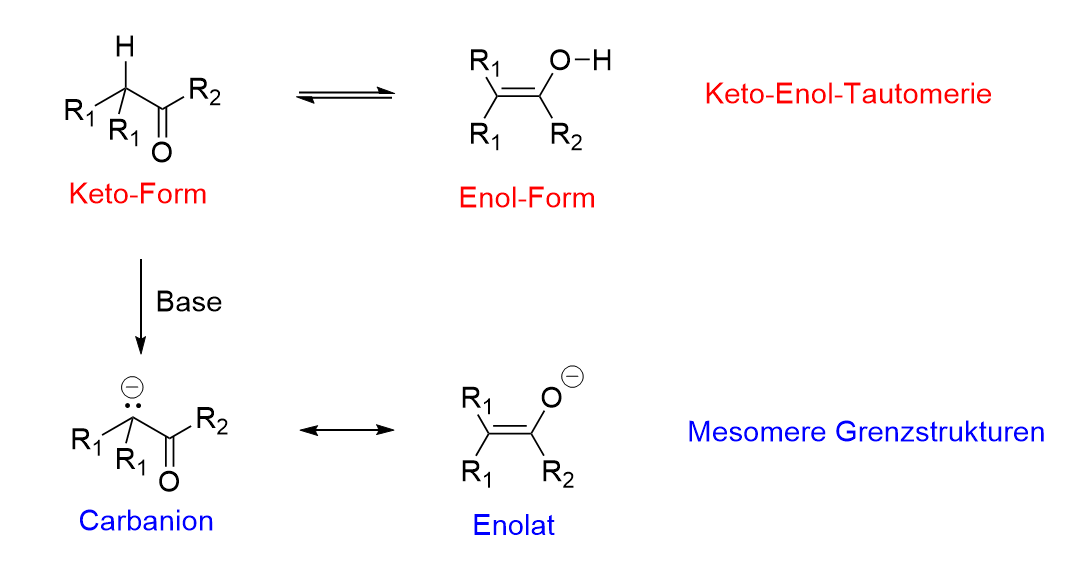
\includegraphics[width=0.9\linewidth]{Bilder/Keto-Enol-Tautomerie.png}
\end{figure}
Die Gleichgewichtslage bei Keto-Enol-Tautomerie ist abhängig von Substituenten und Lösemittel.
In Polaren Lösemitteln überwiegt die Keto-Form, in unpolaren die Enol-Form.

\subsubsection{Erzeugung von Nucleophilen Kohlenstoffen über Enolate}
Die Erzeugung von Enolaten erfolgt über die Deptrotonierung des $\alpha$-H-Atoms. Benachbarte Elektronenziehende Gruppen stabilisieren das Enolat und sorgen für eine leichtere Deprotonierung.
\begin{figure}[H]
	\centering
	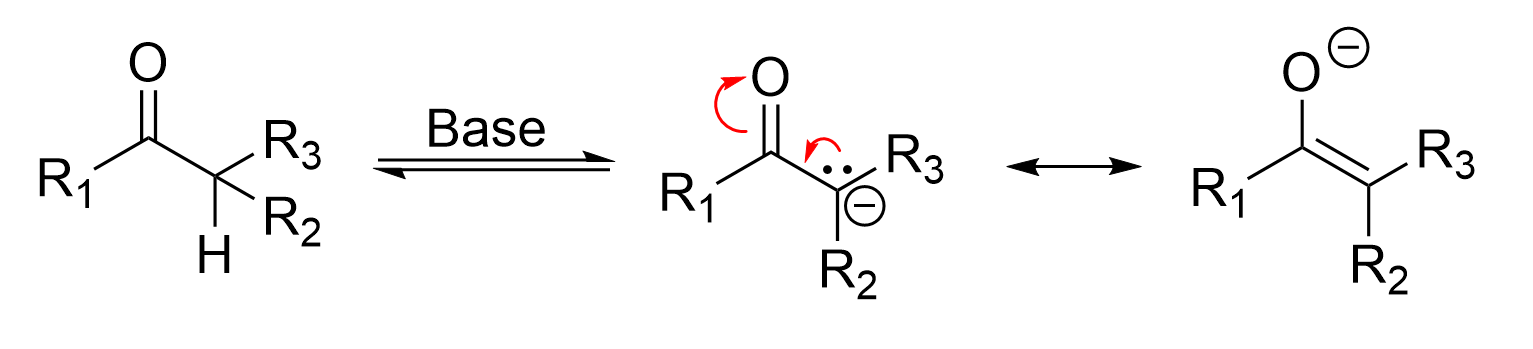
\includegraphics[width=0.8\linewidth]{Bilder/Reaktionen über Enolate.png}
\end{figure}
\noindent Es gilt die Regel: Eine CH-Säure wird von einer äquimolaren Base zum größten Teil deprotoniert, wenn der pKs der CH-Säure kleiner ist als der pKs der konjugierten Säure der Base. Nicht Nucleophile Basen sind LTMP, LDA, LiHMDS, Nucleophile Basen sind t-BuLi, s-BuLi, n-BuLi und PhLi.

\subsubsection{Halogenierung}
\subsubsection*{Basenkatalysiert}
\begin{figure}[H]
	\centering
	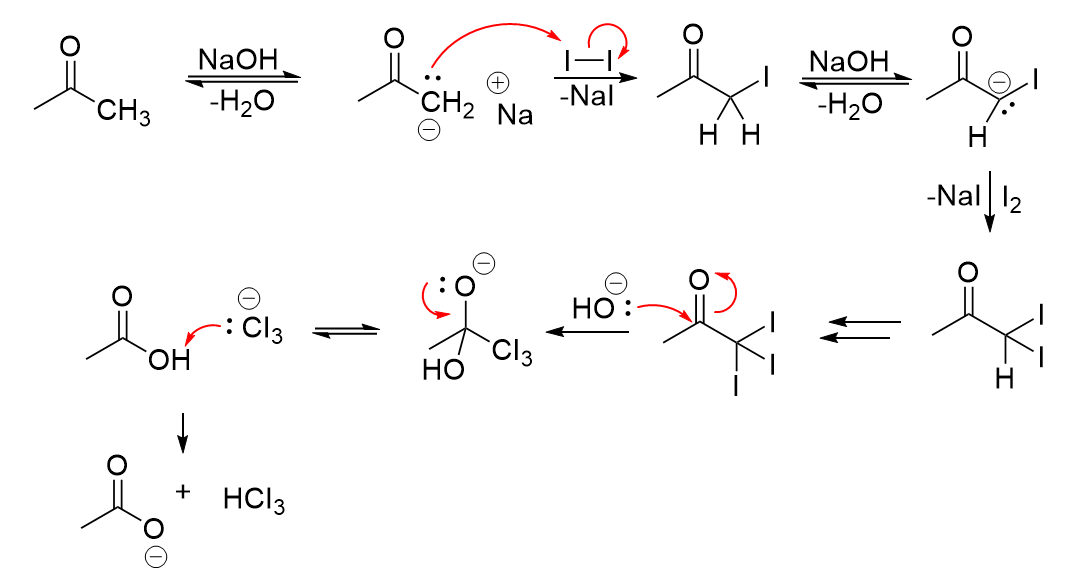
\includegraphics[width=0.95\linewidth]{Bilder/Basenkatalysierte Idoform Bildung.png}
\end{figure}
\subsubsection*{Säurekatalysiert}
\begin{figure}[H]
	\centering
	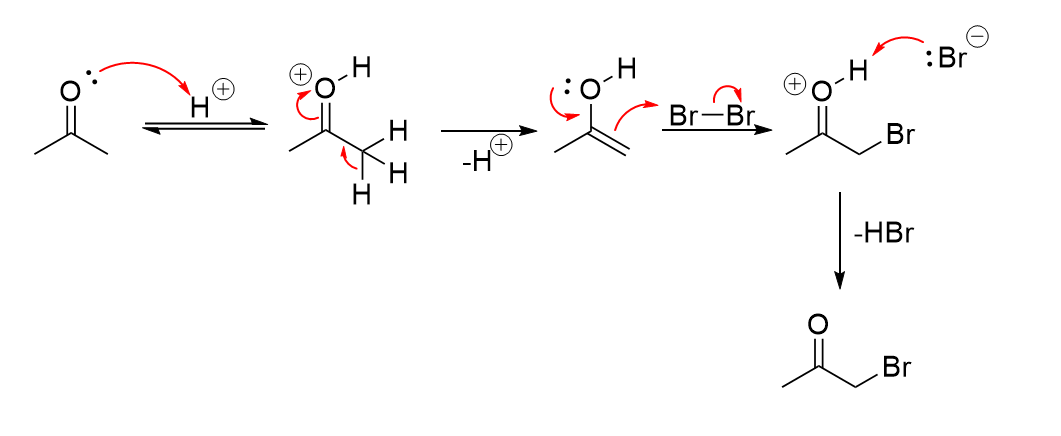
\includegraphics[width=0.95\linewidth]{Bilder/Halogenierung Enole Sauer.png}
\end{figure}
Im Sauren entsteht nur das Monohalogenierte Produkt, da der -I Effekt des Halogenids verhindert, dass das Elektronenpaar der C=O Doppelbindung zum Sauerstoff klappt.

\subsubsection{Mannich Reaktion}
Ês handelt sich um eine Aminomethylierung (rot) und häufig mit einer nachfolgenden Hoffmann Eliminierung (blau).
\begin{figure}[H]
	\centering
	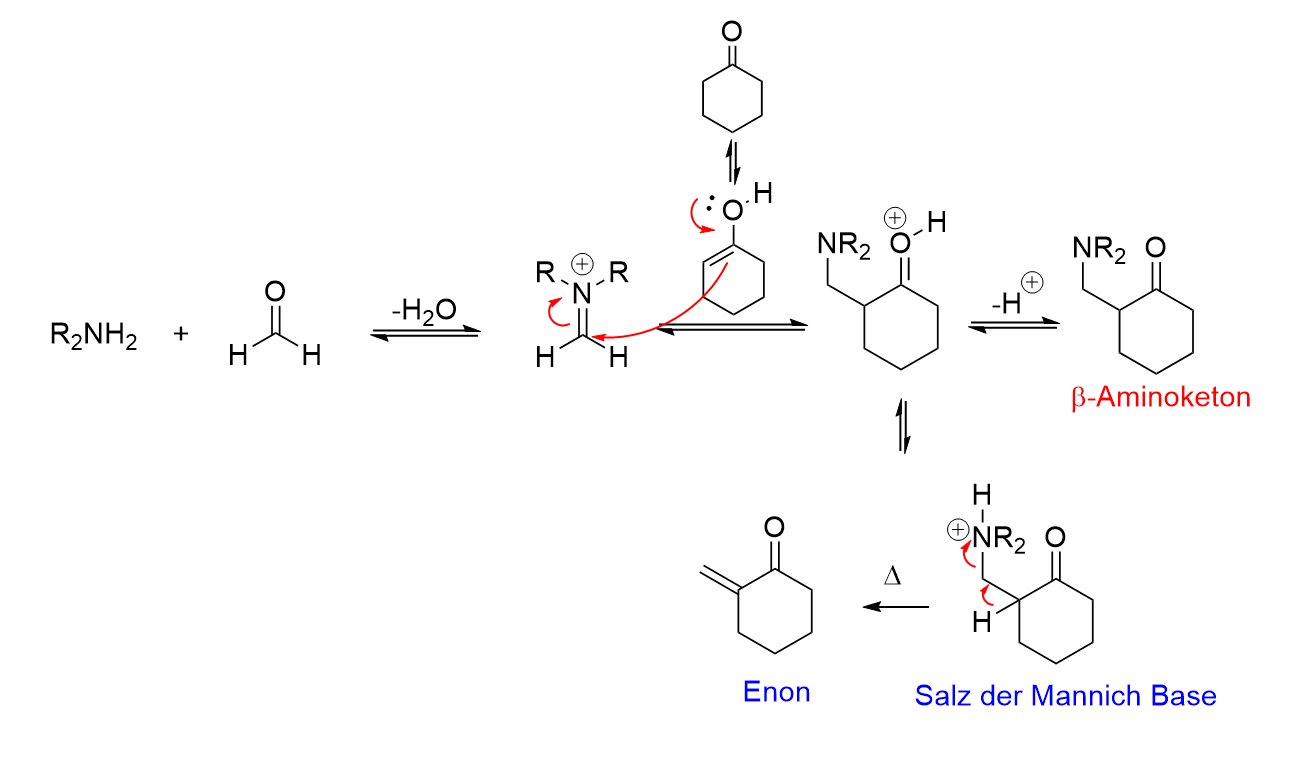
\includegraphics[width=1.0\linewidth]{Bilder/Mannich.png}
\end{figure}

\subsubsection{Aldol Kondensation}
\subsubsection*{Basenkatalysiert}
\begin{figure}[H]
	\centering
	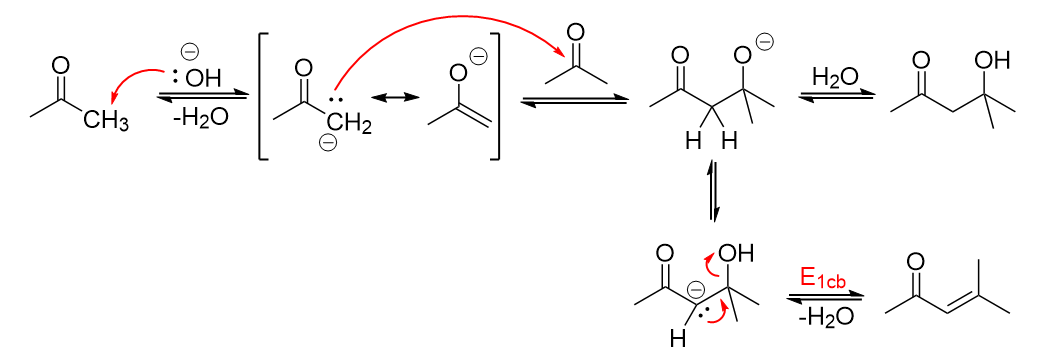
\includegraphics[width=1.0\linewidth]{Bilder/Aldol Basenkatalysiert.png}
\end{figure}
\subsubsection*{Säurekatalysiert}
\begin{figure}[H]
	\centering
	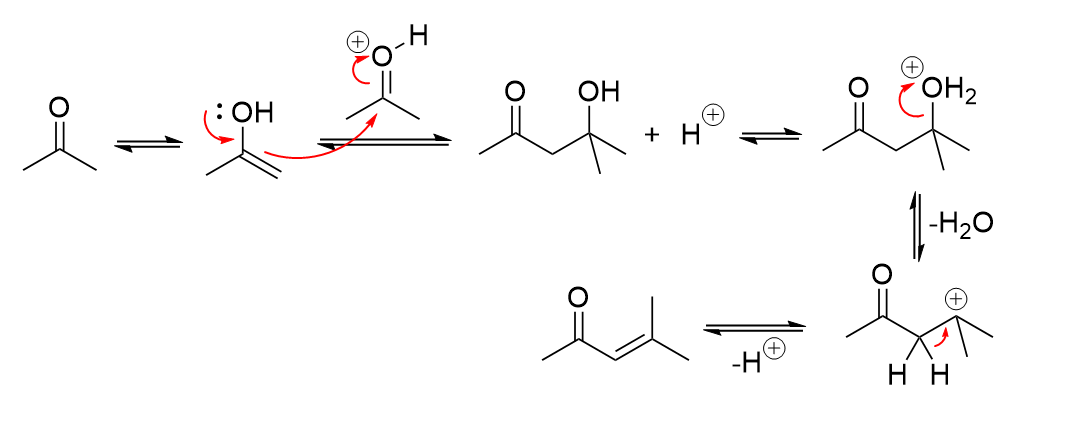
\includegraphics[width=1.0\linewidth]{Bilder/Aldolkondensation Säurekatalysiert.png}
\end{figure}

\subsubsection{Gekreuzte Aldolkondensation}
 Bei der gekreuzten Aldolkondensation können bis zu 4 Aldolprodukte entstehen. Um dies zu verhindern ist eine Carbonyl-Komponente \textbf{Enolisierbar} und die andere \text{nicht}. Nicht Enolisierbar ist zum Beispiel Benzaldehyd, da hier keine $\alpha$-CH-Acidität vorliegt.




\subsubsection{Claisen'sche Ester Kondensation}
\begin{figure}[H]
	\centering
	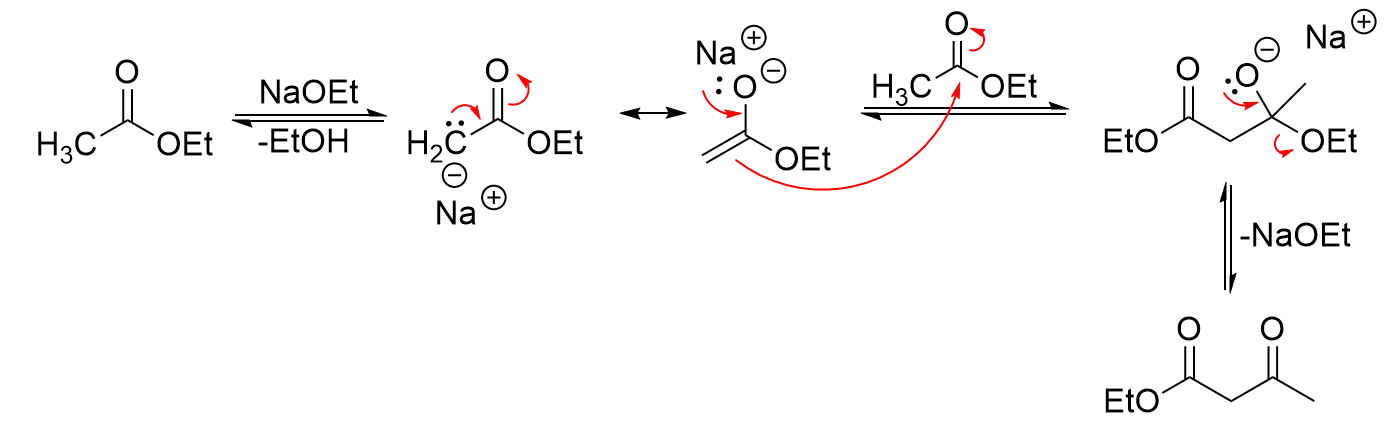
\includegraphics[width=1.0\linewidth]{Bilder/Claisen Kondensation.png}
\end{figure}


\subsubsection{Dieckmann-Kondensation}
\begin{figure}[H]
	\centering
	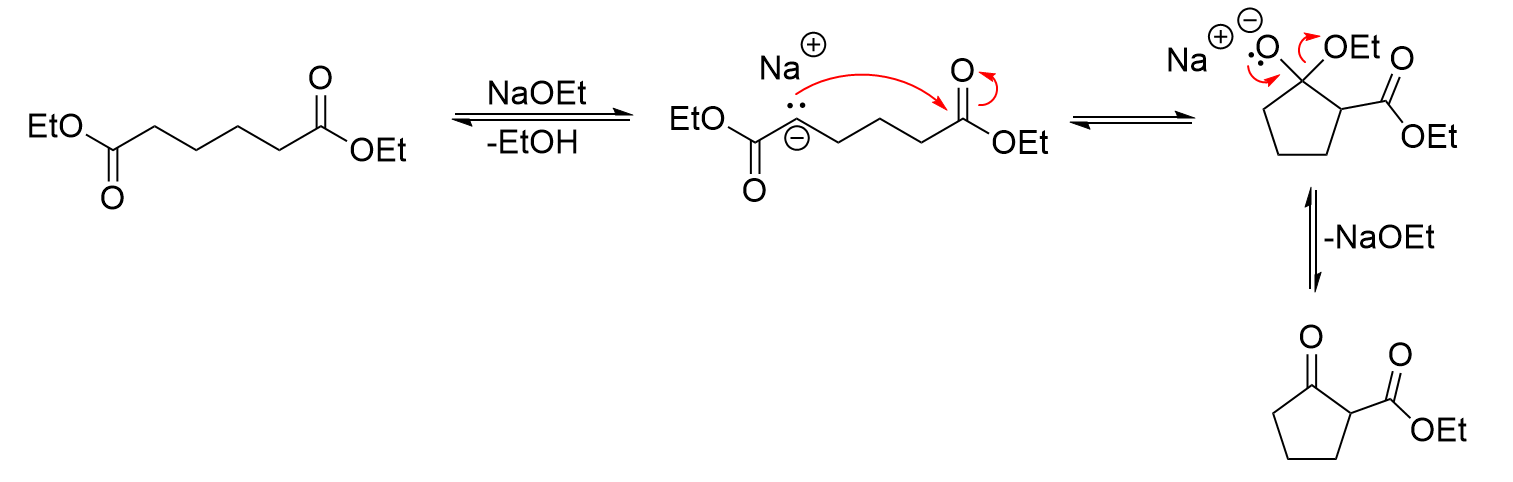
\includegraphics[width=1.0\linewidth]{Bilder/Dieckmann-Kondensation.png}
\end{figure}

\subsubsection{Acetessigester-Synthese}
Es handelt sich nicht um die Synthese von Acetessigester sondern dieser wird hier als Edukt verwendet! Die Reaktion bildet aus Claisen'schen-Ester-Kondensations-Produkten Ketone.
\begin{figure}[H]
	\centering
	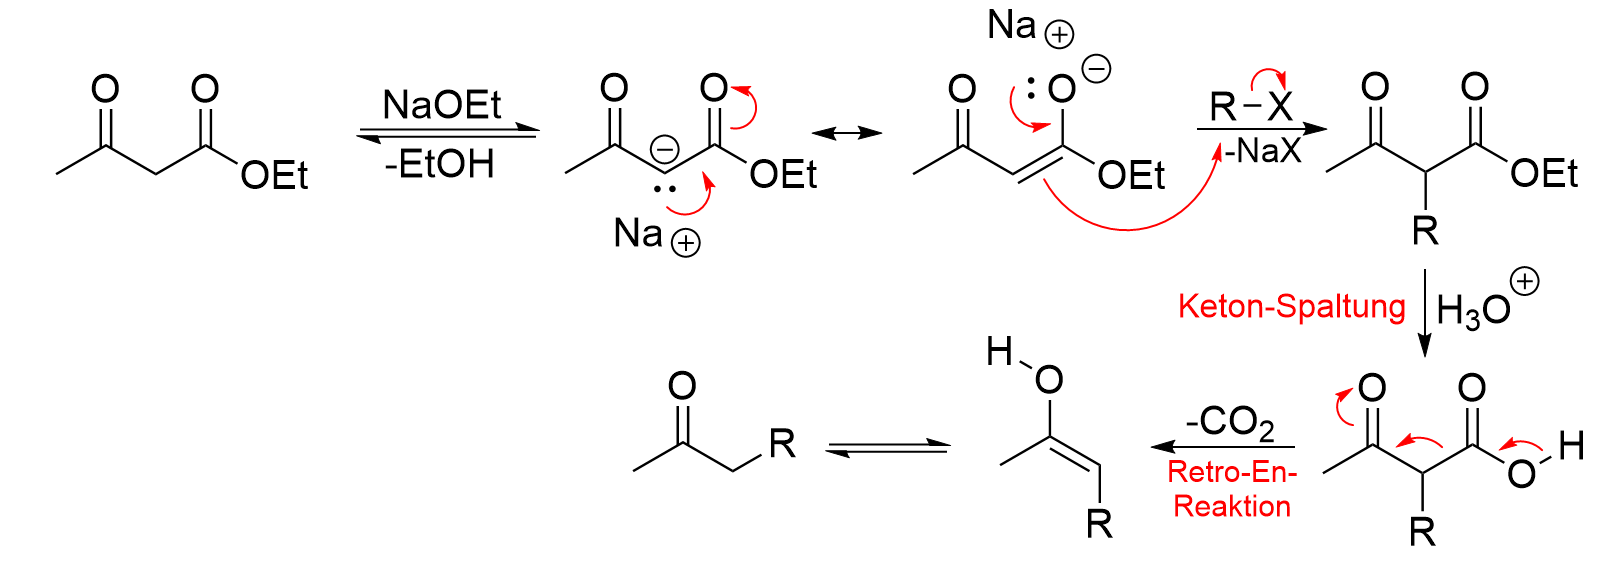
\includegraphics[width=1.0\linewidth]{Bilder/Acetessigester Synthese.png}
\end{figure}

\subsubsection{Säurespaltung von Claisen-Ester-Kondensations-Produkten}
\begin{figure}[H]
	\centering
	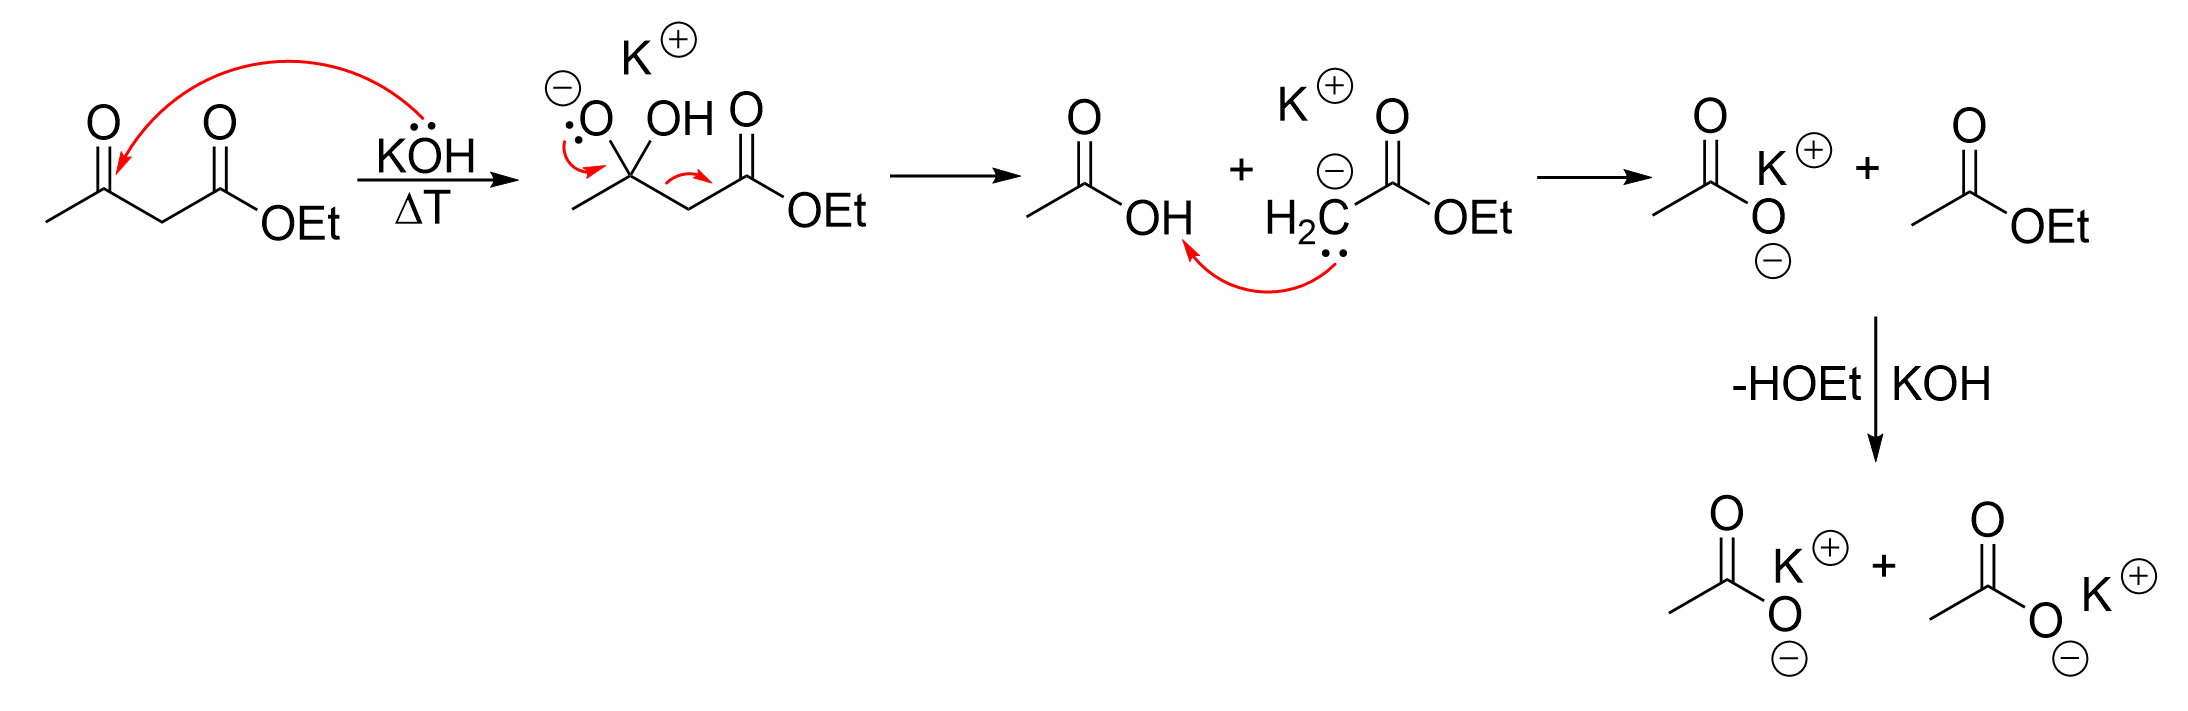
\includegraphics[width=1.0\linewidth]{Bilder/Säurespaltung Claisen_Ester.png}
\end{figure}

\subsubsection{Malonester-Synthese}
\begin{figure}[H]
	\centering
	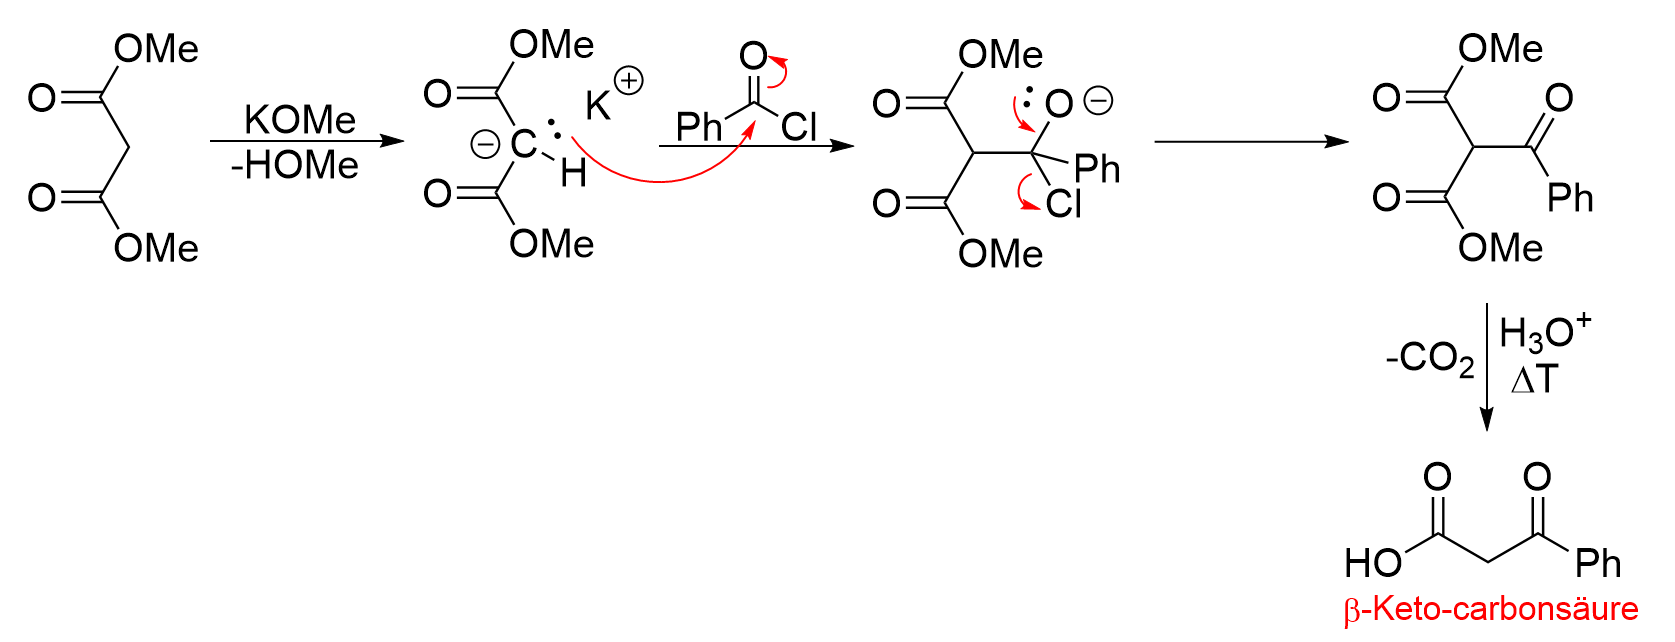
\includegraphics[width=1.0\linewidth]{Bilder/Malonester-Synthese.png}
\end{figure}


\subsubsection{Darzens-Glycidester-Synthese}
\begin{figure}[H]
	\centering
	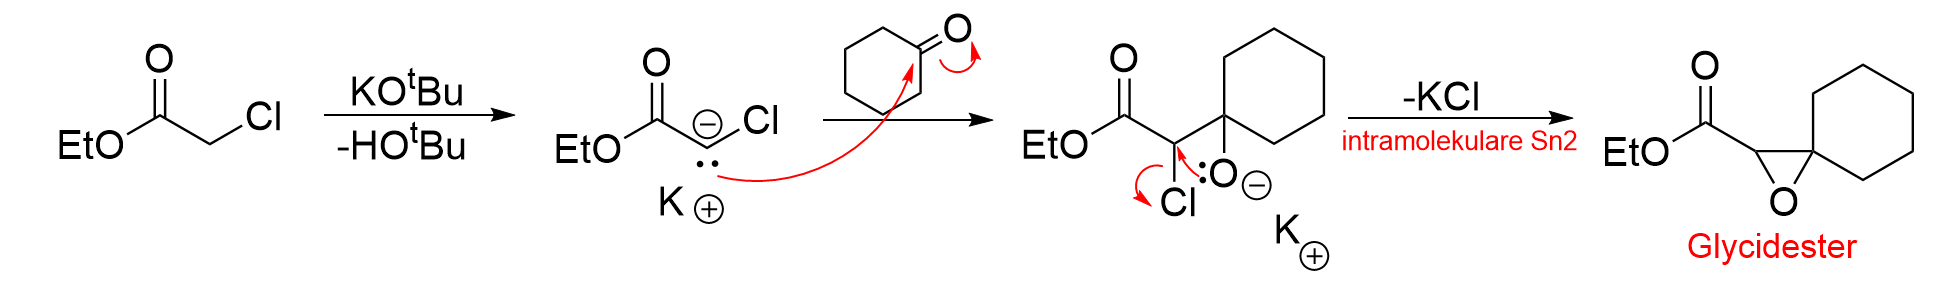
\includegraphics[width=1.0\linewidth]{Bilder/Darzens Glycidester Synthese.png}
\end{figure}

\subsubsection{Knoevenhagel-Reaktion}
\subsubsection*{Allgemein}
\begin{figure}[H]
	\centering
	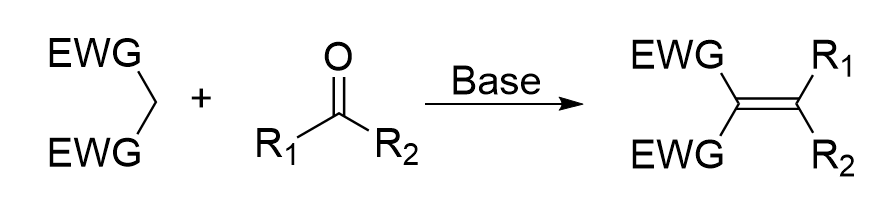
\includegraphics[width=0.6\linewidth]{Bilder/knoevenhagel allgemein.png}
\end{figure}
\subsubsection*{Mechanismus}
\begin{figure}[H]
	\centering
	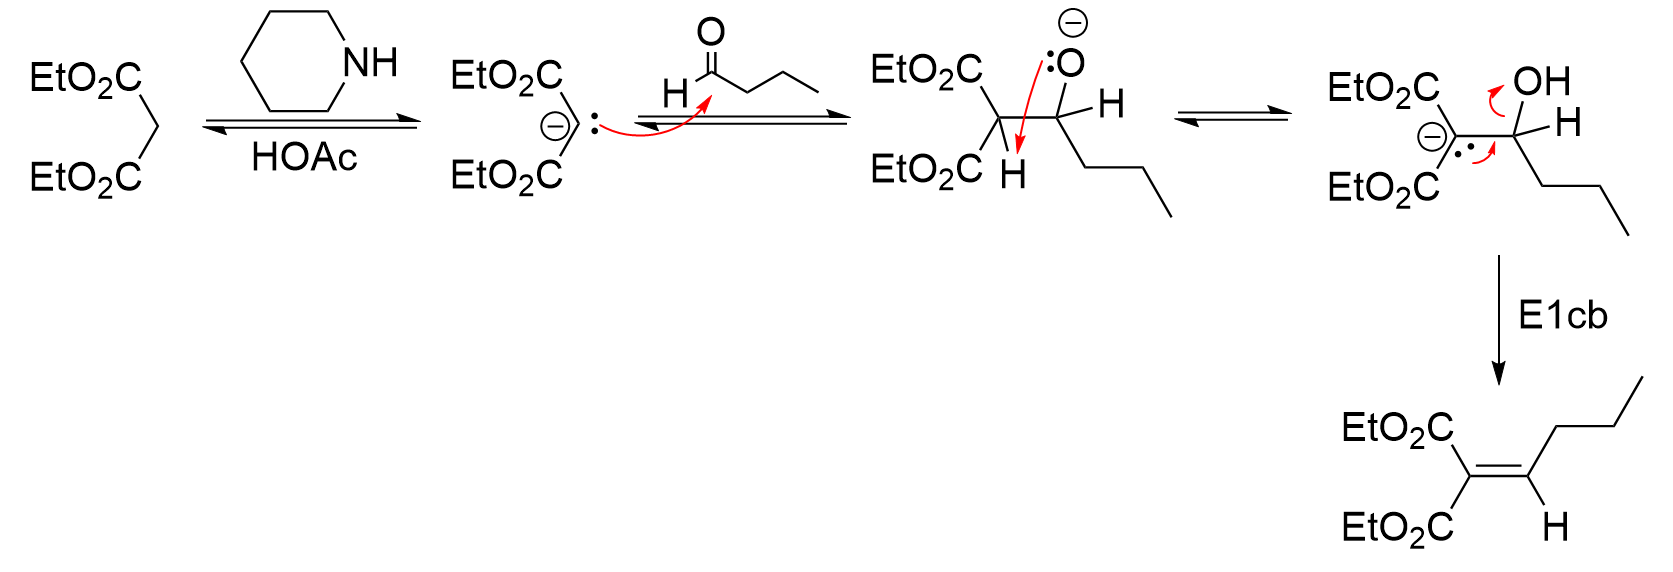
\includegraphics[width=1.0\linewidth]{Bilder/Knoevenhagel.png}
\end{figure}


\subsubsection{Michael Reaktion}
\begin{figure}[H]
	\centering
	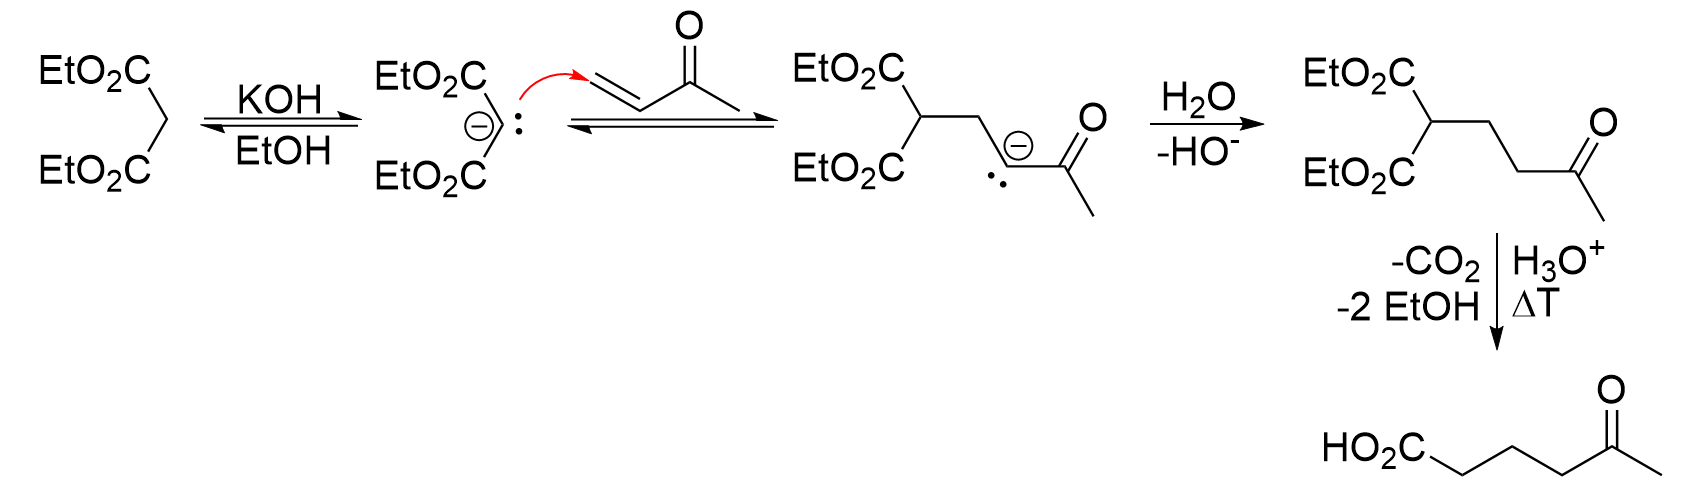
\includegraphics[width=1.0\linewidth]{Bilder/Michael Addition.png}
\end{figure}



\subsubsection{Robinson Anellierung}
\begin{figure}[H]
	\centering
	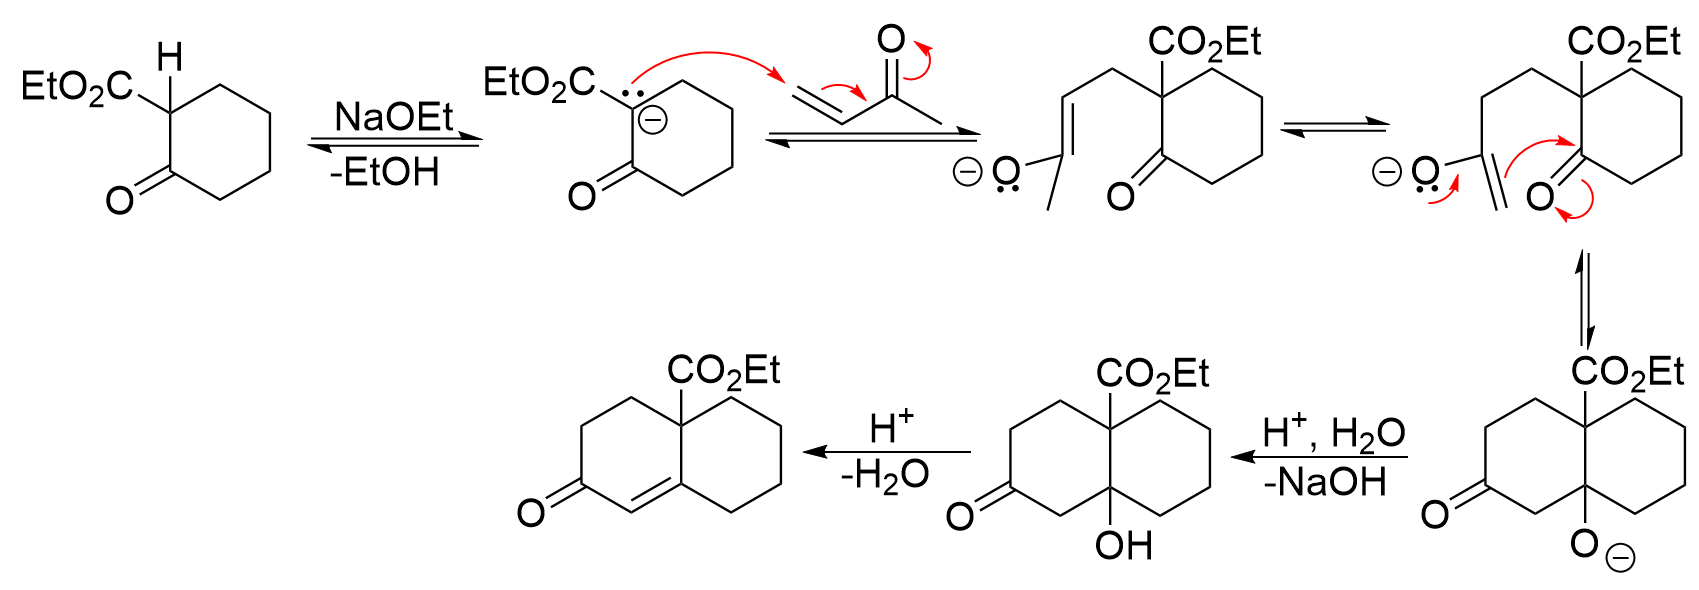
\includegraphics[width=1.0\linewidth]{Bilder/Robinson Anellierung.png}
\end{figure}






%\subsubsection{Henry-Reaktion}
%Sie hat dies nur in Folie gezeigt -> irrelevant?

\newpage
\section{Metallorganische Verbindungen}
Metallorganische Verbindungen liegen nicht in der einfachen Schreibweise R-M, wobei M das Metall ist, vor.
Stattdessen liegen sie als Aggregate in Lösung vor. 
\begin{figure}[H]
	\centering
	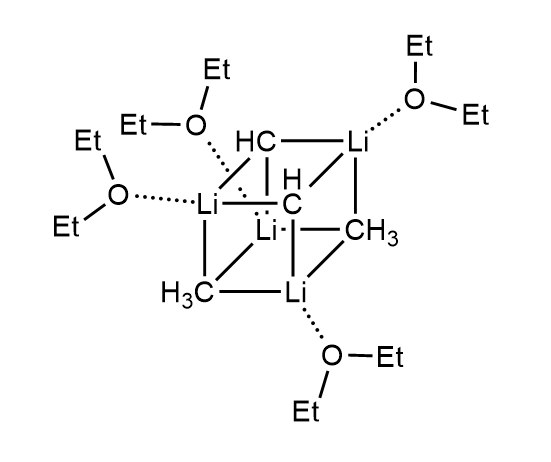
\includegraphics[width=0.4\linewidth]{Bilder/Tetramer MeLi.png}
	\caption{Tetramer des MeLi in Diethylether. Die Schreibweise bedeutet nicht, dass Kohlenstoff sechsbindig ist.}
\end{figure}
\noindent Das Aggregat sorgt dafür, dass jedes Metallkation seinen Elektronenmangel verringern kann.
Neben Tetrameren können auch andere Geometrien vorkommen wie zum Beispiel Tetraeder.
\begin{figure}[H]
	\centering
	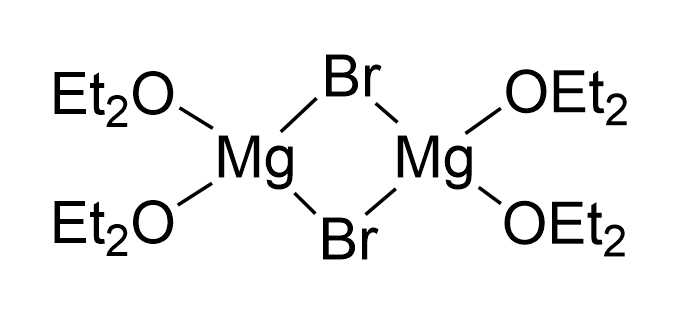
\includegraphics[width=0.3\linewidth]{Bilder/Dimer EtMgBr.png}
	\caption{Dimer von EtMgBr.}
\end{figure}

\subsection{Reaktionen}
\subsubsection{Hydrolyse}
\begin{equation*}
	\ce{n-BuLi + H2O -> LiOH + n-BuH}
\end{equation*}
\subsubsection*{Deuterierung über Grignard}
\begin{figure}[H]
	\centering 
	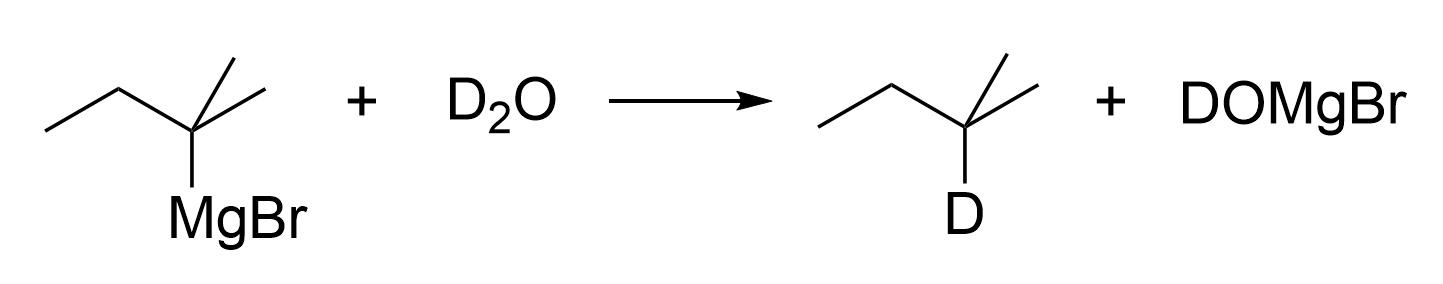
\includegraphics[width=0.7\linewidth]{Bilder/Deuterierung Grignard.png}
\end{figure}

\subsubsection{Oxidation}
\ce{Et2Zn}, \ce{Me3B}, \ce{Me3Al} sind pyrophor. \ce{MeLi}, \ce{n-BuLi}, \ce{RMgBr} sind nur in Lösung unter Schutzgas handhabbar.

\subsubsection{Reaktionen als C-Nucleophile}
\begin{figure}[H]
	\centering 
	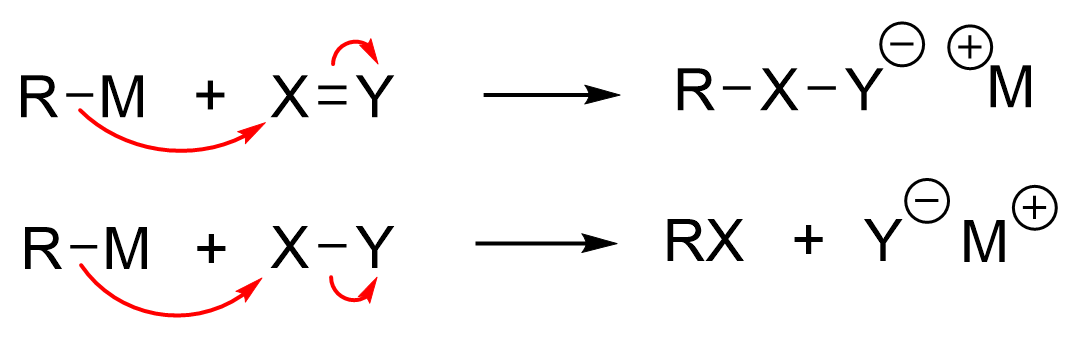
\includegraphics[width=0.5\linewidth]{Bilder/reaktion als c nucleophil.png}
\end{figure}



\section{Carbonsäuren und Derivate}
\subsection{Stoffchemie der Carbonsäuren}
\subsubsection*{Ameisensäure}
\begin{figure}[H]
	\centering 
	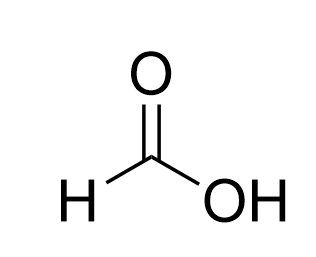
\includegraphics[width=0.15\linewidth]{Bilder/ameisensäure.png}
\end{figure}
Die Ameisensäure weißt neben ihrer Carbonsäure-Gruppe noch einen Wasserstoff als Substituenten auf. Dadurch kann die Ameisensäure ebenso als Reduktionsmittel wirken.


\subsubsection*{Seifen}
Seifen sind Alkalisalze langkettiger Carbonsäuren. Sie besitzen einen hydrophilen und einen hydrophoben Rest und sind daher amphiphil. Kernseifen sind Natriumsalze und Schmierseifen sind Kaliumsalze.
\begin{figure}[H]
	\centering 
	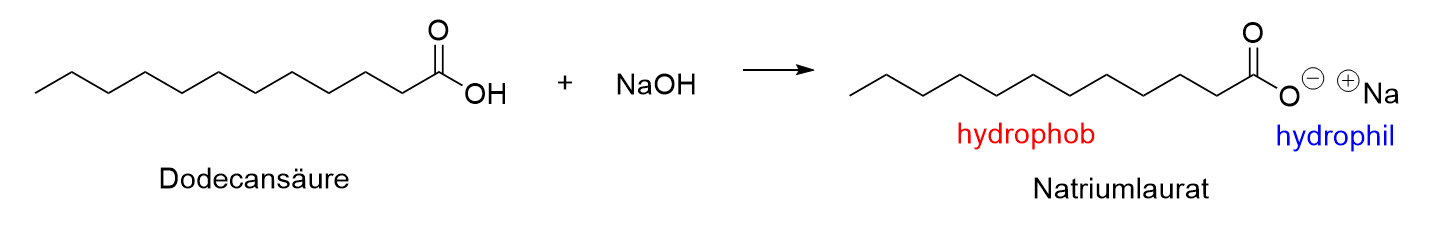
\includegraphics[width=1\linewidth]{Bilder/Laurat.png}
	\caption{Natriumlaurat aus Dodecansäure.}
\end{figure}
\noindent Neben solchen Anionenseifen gibt es auch Kationenseifen z.B aus Aminen.
Die Darstellung von Carbonsäuren kann über Esterhydrolyse, Oxidation von Alkoholen und Methylaromaten und über das abfangen von Metallorganischen Verbindungen mit \ce{CO2} erfolgen.
Oxidationsmittel für die Oxidation von Alkoholen zu Carbonsäuren ist z.B Natriumdichromat.


\subsubsection*{Carbonsäurehalogenide}
Bei den Säurehalogeniden sind oft nur die Chloride in Verwendung. Alle anderen Halogene sind selten.
\begin{figure}
	\centering
	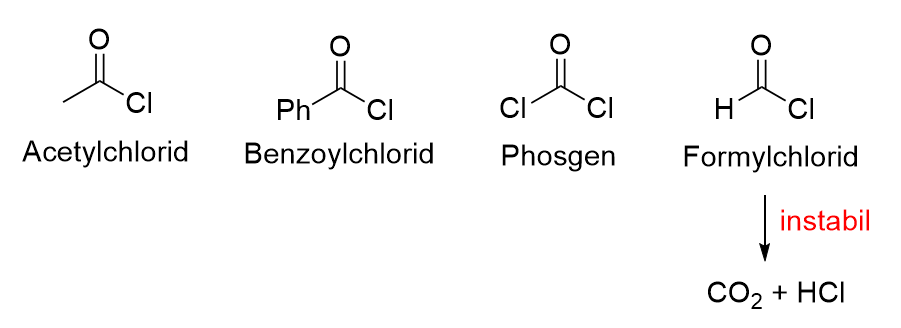
\includegraphics[width=0.7\linewidth]{Bilder/Carbonsäurechloride}
\end{figure}
Carbonsäurechloride sind die reaktivste Substanzklasse aller Carbonylverbindungen und Carbonsäuren, da das Chlor und das Carbonyl-Sauerstoff die Carbonylaktivität stark erhöhen.

\subsubsection*{Amide}
Amide kommen vorallem in Proteinen und in synthetischen Polyamiden (Kunststoffen) vor.




\subsection{Carbonsäuren}
\subsubsection{Allgemeine Reaktionsmöglichkeiten von Carbonsäuren}
\begin{figure}[H]
	\centering 
	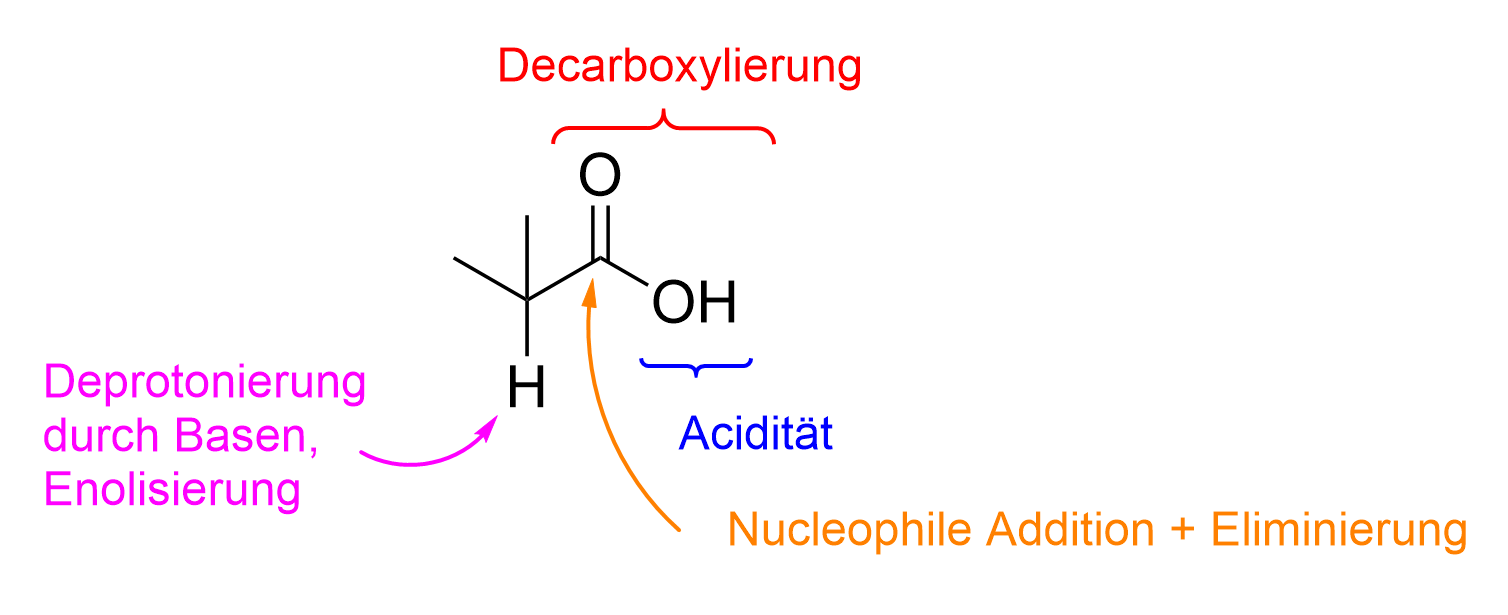
\includegraphics[width=0.7\linewidth]{Bilder/Carbonsäuren Reaktionen allgemeines.png}
\end{figure}

\subsubsection{Hunsdiecker-Reaktion (Decarboxylierung)}
\begin{figure}[H]
	\centering 
	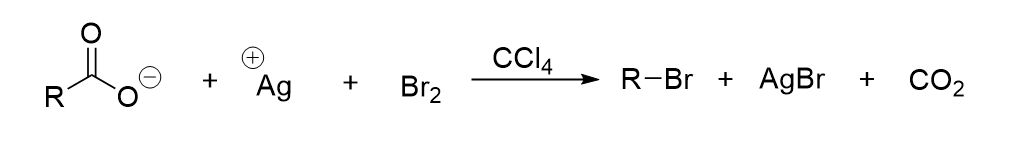
\includegraphics[width=1.0\linewidth]{Bilder/Hunsdiecker Bilanzgleichung.png}
\end{figure}

\subsubsection*{Mechanismus}
\begin{figure}[H]
	\centering 
	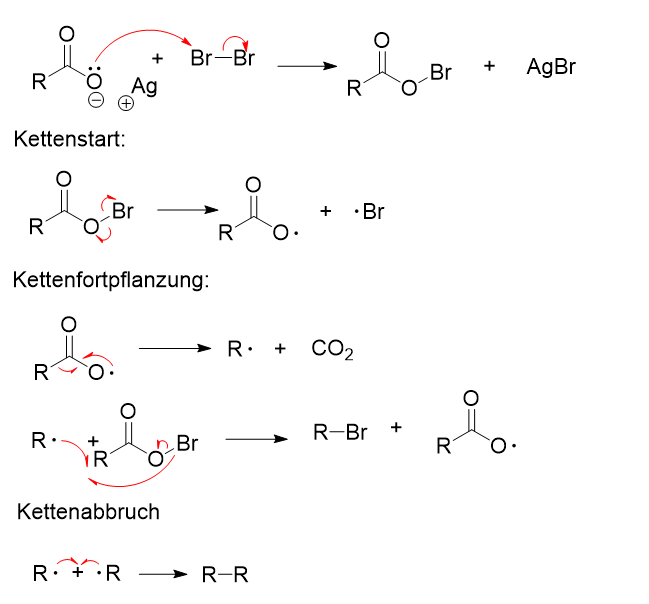
\includegraphics[width=0.75\linewidth]{Bilder/Hunsdiecker.png}
\end{figure}

\subsubsection{Decarboxylierung von $\beta$-Ketosäuren}
Carbonylgruppen in Nachbarstellung zu Carbonsäuren begünstigen die Decarboxylierung.
\begin{figure}[H]
	\centering 
	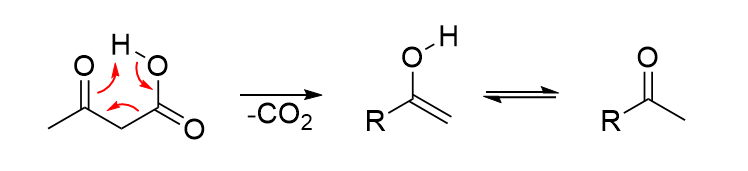
\includegraphics[width=0.75\linewidth]{Bilder/Decarboxylierung von beta-Ketosäuren.png}
\end{figure}



\subsection{Ester und Amide}
\subsubsection{Veresterung mit Diazomethan}
\subsubsection*{Darstellung von Diazomethan}
\begin{figure}[H]
	\centering 
	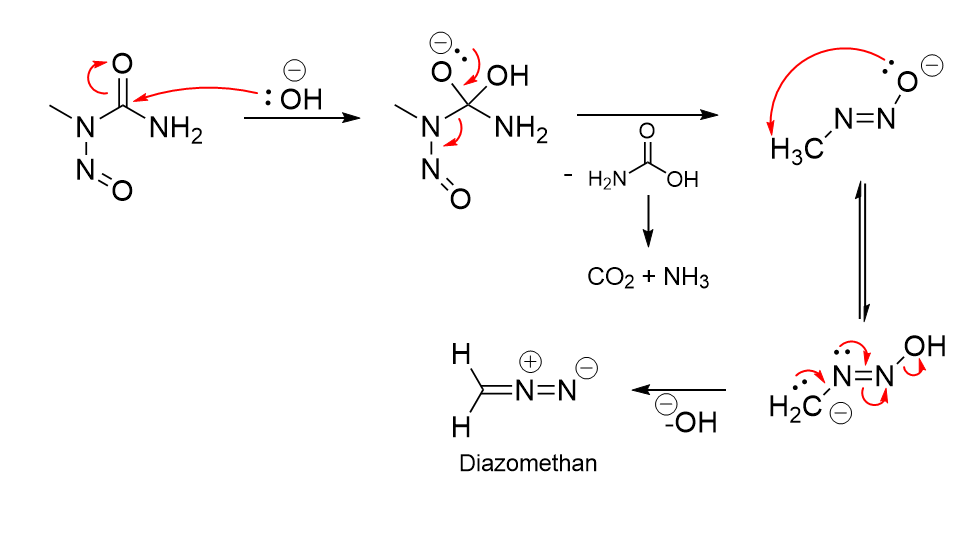
\includegraphics[width=0.8\linewidth]{Bilder/Darstellung von Diazomethan.png}
\end{figure}
\subsubsection*{Veresterung mit Diazomethan}
\begin{figure}[H]
	\centering 
	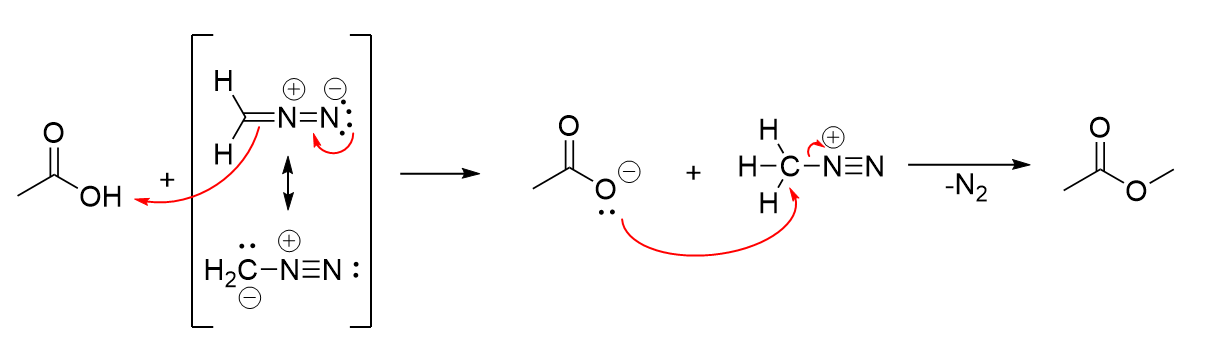
\includegraphics[width=1\linewidth]{Bilder/Veresterung mit Diazomethan.png}
\end{figure}
Die Veresterungsmethode ist mild unter neutralen Bedingungen und daher für Naturstoffisolierung sehr gut geeignet.

\subsubsection{Bildung des tert-Butylesters als Schutzgruppe}
\begin{figure}[H]
	\centering 
	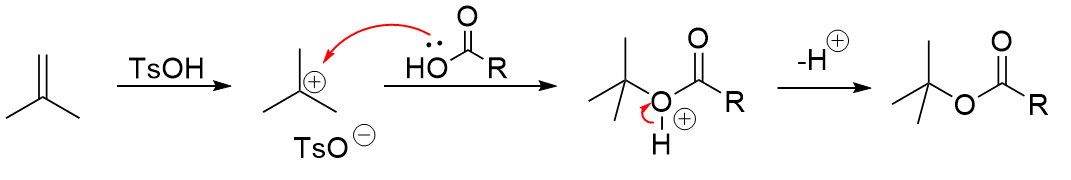
\includegraphics[width=1\linewidth]{Bilder/tertButylester als Schutzgruppe.png}
\end{figure}
\subsubsection{Fischer-Veresterung}
Der Veresterungs-Mechanismus besteht aus einer Abfolge einer Addition und anschließender Eliminierung.
\begin{figure}[H]
	\centering 
	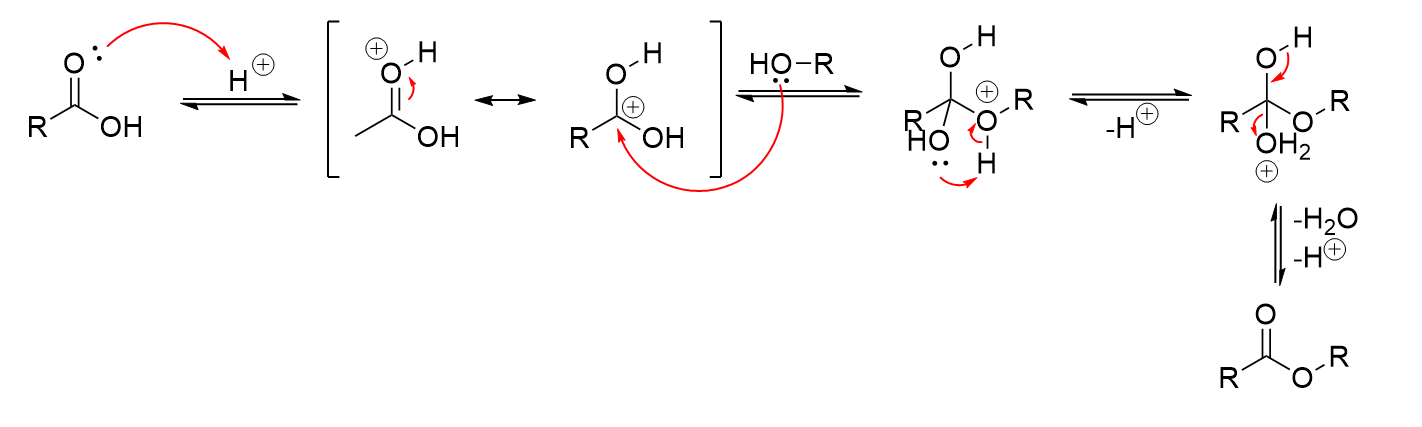
\includegraphics[width=1.1\linewidth]{Bilder/Fischer Veresterung.png}
\end{figure}

\subsubsection{Esterverseifung}
Die Esterverseifung (alkalische Esterhydrolyse) ist irreversibel. Im Säuren liegt ein Gleichgewicht vor, da sie reversibel ist.
\begin{figure}[H]
	\centering 
	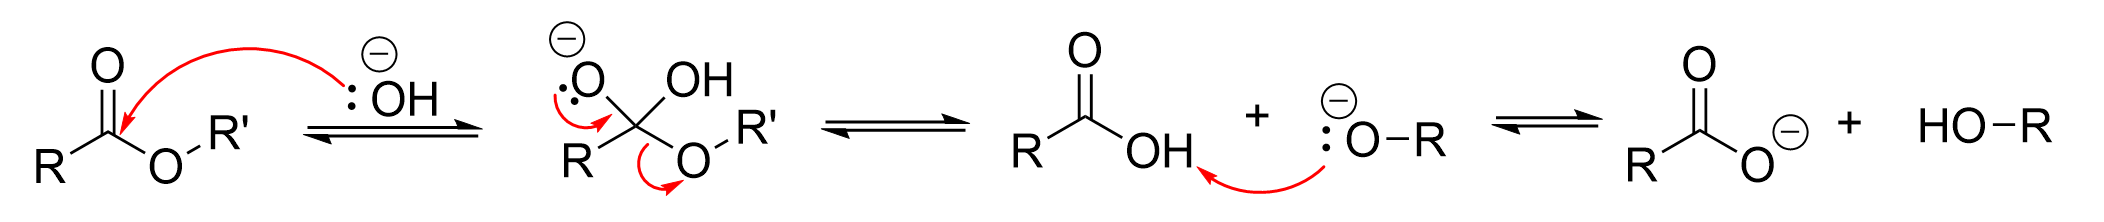
\includegraphics[width=1.0\linewidth]{Bilder/Esterverseifung.png}
\end{figure}


\subsubsection{Schotten-Baumann-Reaktion}
Die Schotten-Baumann-Reaktion ist eine Veresterung eines Säurehalogenids mit Alkoholen oder aminen zu Estern bzw Amiden.
\begin{figure}[H]
	\centering
	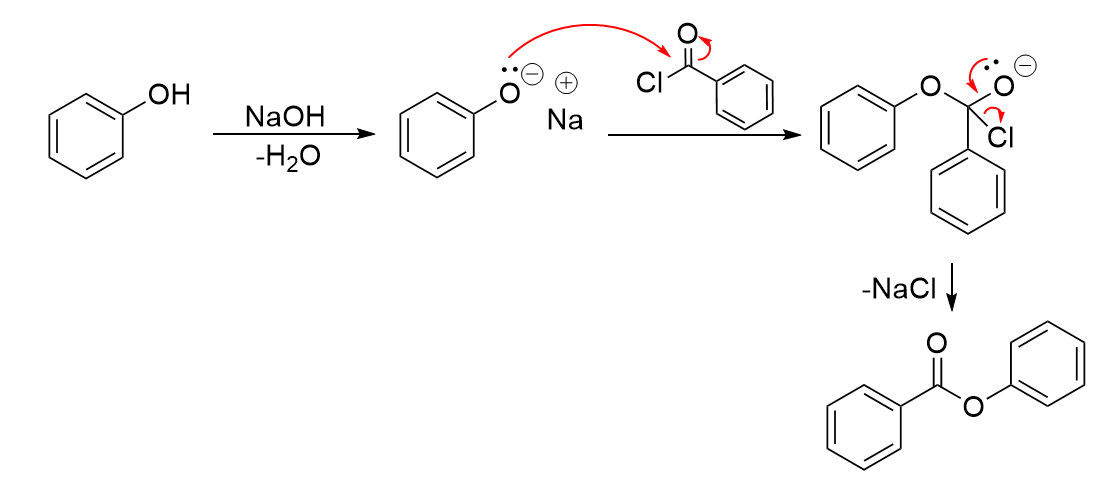
\includegraphics[width=0.8\linewidth]{Bilder/Schotten Baumann Reaktion.png}
\end{figure}

%Amide
\subsubsection{Direkte Amidbildung aus Carbonsäuren}
\begin{figure}[H]
	\centering 
	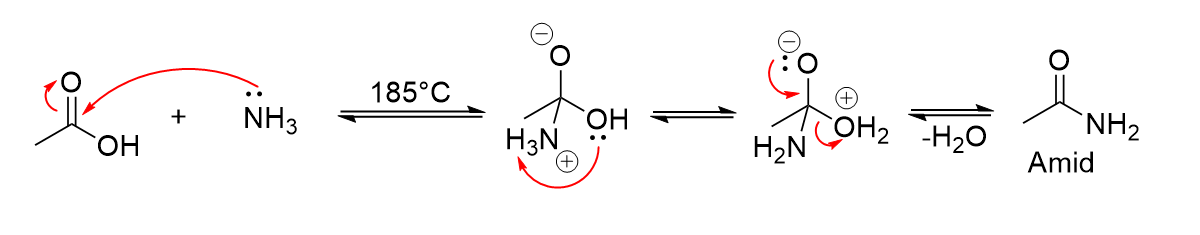
\includegraphics[width=1.0\linewidth]{Bilder/Amidbildung.png}
\end{figure}

\subsubsection{Thermische Zersetzung von Ammoniumcarboxylaten zu Amiden}
\begin{figure}[H]
	\centering 
	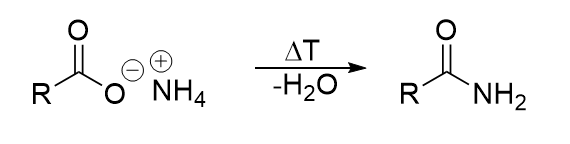
\includegraphics[width=0.6\linewidth]{Bilder/Thermische Zersetzung von Ammoniumcarboxylaten.png}
\end{figure}

\subsubsection{Darstellung von Amiden aus Anhydriden}
\begin{figure}[H]
	\centering 
	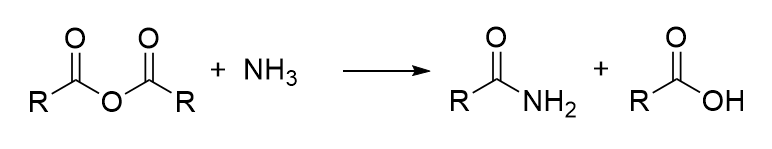
\includegraphics[width=0.6\linewidth]{Bilder/Amide aus Anhydriden.png}
\end{figure}

\subsubsection{Darstellung von Amiden aus Estern}
\begin{figure}[H]
	\centering 
	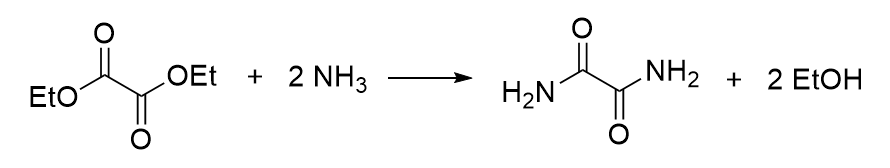
\includegraphics[width=0.65\linewidth]{Bilder/Amide aus Esterns.png}
\end{figure}

\subsubsection{Darstellung von Amiden aus Nitrilen}
\begin{figure}[H]
	\centering 
	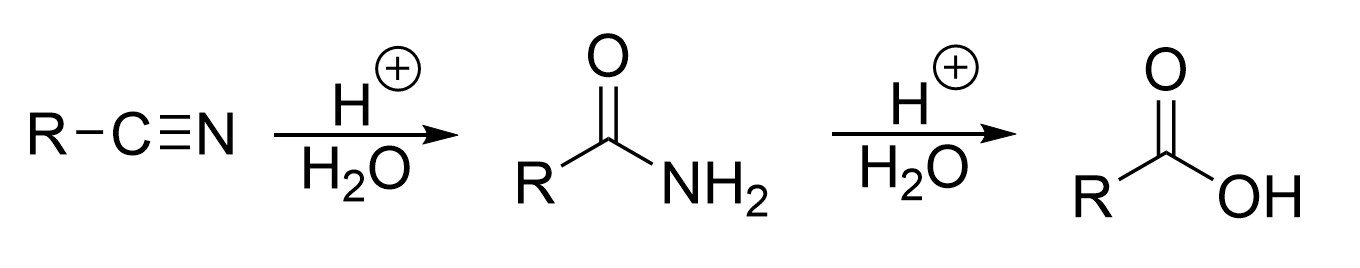
\includegraphics[width=0.6\linewidth]{Bilder/Amide aus Nitrilen.png}
\end{figure}
\subsubsection*{Mechanismus}
\begin{figure}[H]
	\centering 
	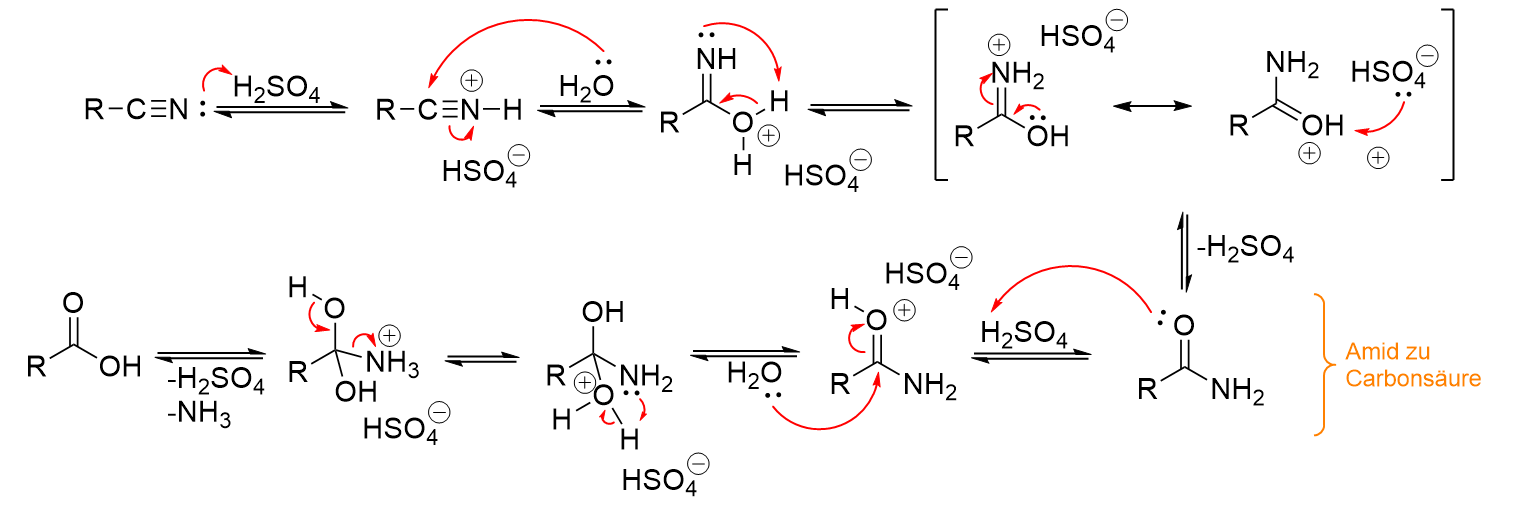
\includegraphics[width=1.1\linewidth]{Bilder/Amide aus Nitrilen-Mechanismus.png}
\end{figure}


\subsection{Carbonsäurehalogenide}
\subsubsection{Darstellung mit Thionylchlorid}
\begin{figure}[H]
	\centering
	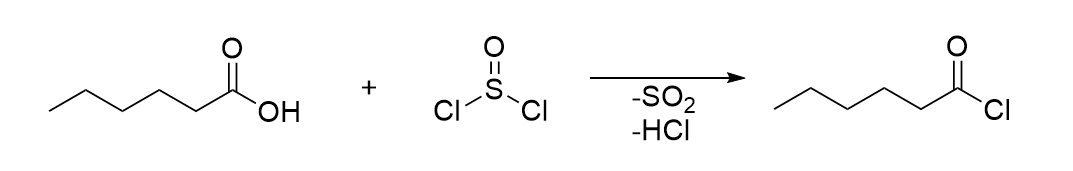
\includegraphics[width=0.9\linewidth]{Bilder/Säurechlorid Thionylchlorid.png}
	%\caption{Darstellung der Säurechloride aus Thionylchlorid}
\end{figure}

\subsubsection{Darstellung mit Oxalylchlorid}
\begin{figure}[H]
	\centering
	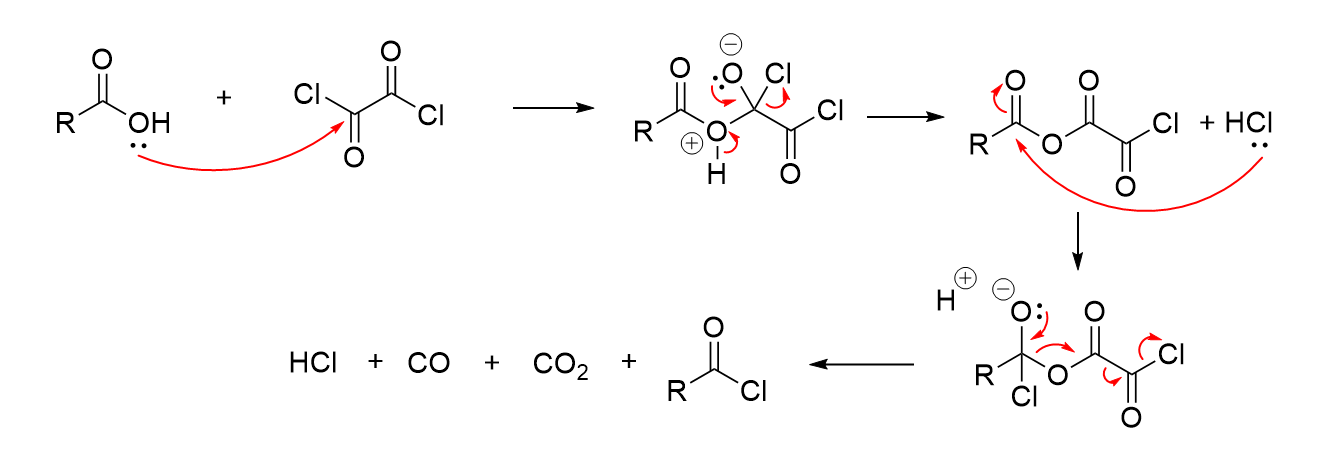
\includegraphics[width=1\linewidth]{Bilder/Säurechlorid Oxalylchlorid.png}
	%\caption{Darstellung der Säurechloride aus Oxalylchlorid}
\end{figure}

\subsubsection{Darstellung mit Phosphorpentachlorid}
\begin{figure}[H]
	\centering
	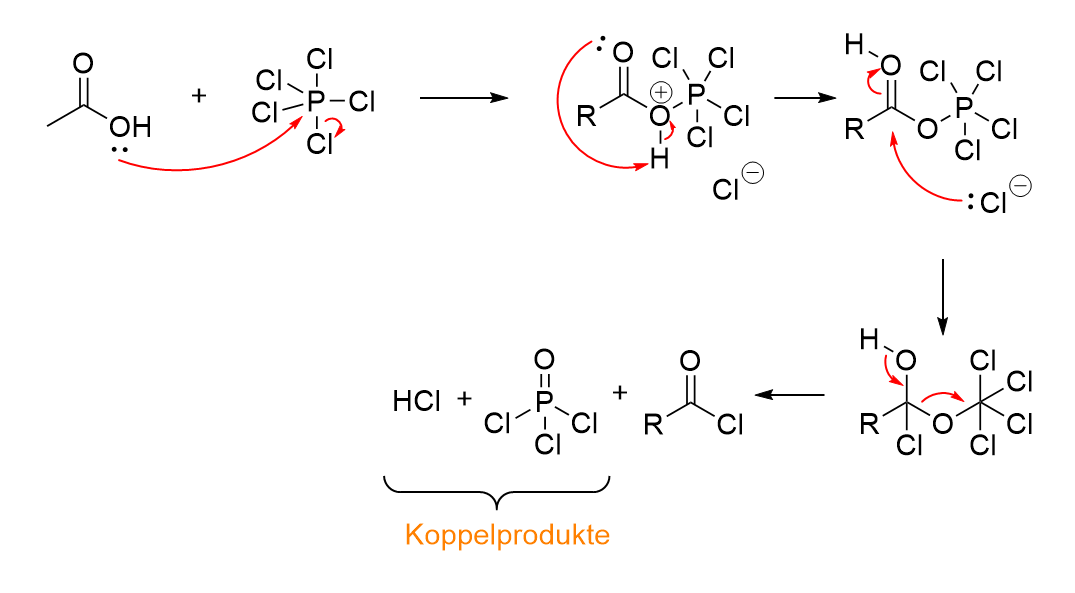
\includegraphics[width=0.85\linewidth]{Bilder/Säurechloride Phosphorpentachlorid.png}
	%\caption{Darstellung der Säurechloride aus Phosphorpentachlorid}
\end{figure}

\subsubsection{Halogenidaustausch der Säurehalogenide}
\begin{figure}[H]
	\centering
	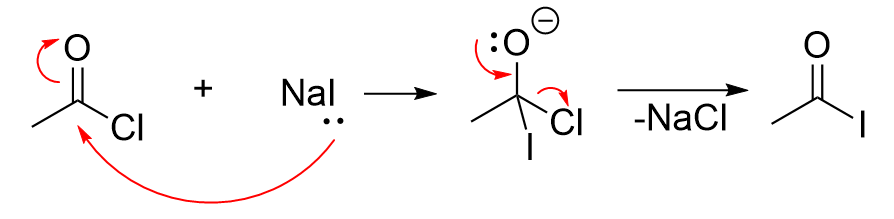
\includegraphics[width=0.65\linewidth]{Bilder/Säurechloride Halogenidaustausch.png}
	%\caption{Halogenidaustausch der Säurechloride}
\end{figure}

\subsection{Anhydride}
\subsubsection{Darstellung mit Phosphorpentoxid}
\begin{figure}[H]
	\centering
	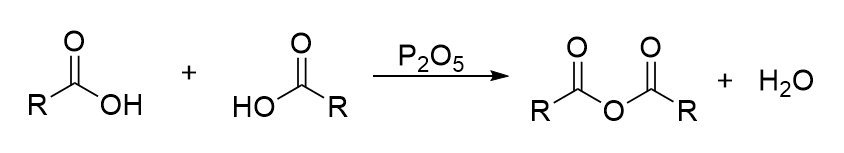
\includegraphics[width=0.75\linewidth]{Bilder/anhydride aus Phosphorpentoxid.png}
	%\caption{Darstellung von Säureanhydriden aus Phosphorpentoxid}
\end{figure}

\subsubsection{Darstellung aus Säurehalogeniden}
\begin{figure}[H]
	\centering
	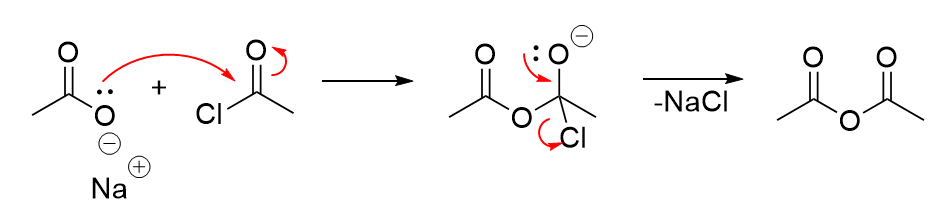
\includegraphics[width=0.8\linewidth]{Bilder/anhydride aus Säurechloride.png}
	%\caption{Darstellung von Säureanhydriden aus Säurechloriden}
\end{figure}

\subsubsection{Darstellung von Anhydriden über in situ Aktivierung}
\begin{figure}[H]
	\centering
	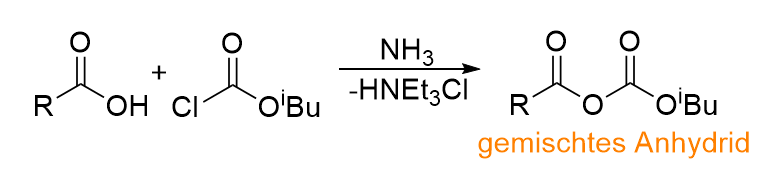
\includegraphics[width=0.75\linewidth]{Bilder/Anhydride in situ aktivierung.png}
	%\caption{Darstellung von gemischten Anhydriden über in situ Aktivierung}
\end{figure}

\subsection{Hydrazide}
\subsubsection{Stoffchemie}
\begin{figure}[H]
	\centering
	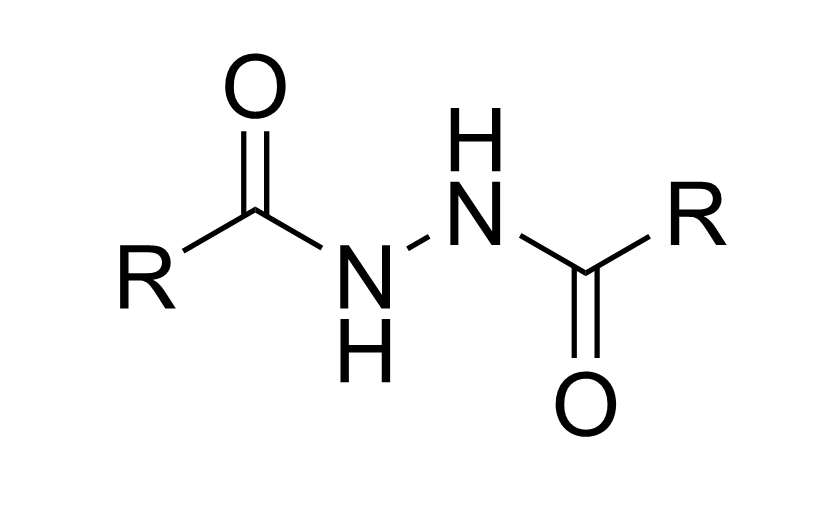
\includegraphics[width=0.25\linewidth]{Bilder/Hydrazide Stoffchemie.png}
\end{figure}

\subsubsection{Hydrazinolyse bei der Gabriel-Synthese}
\begin{figure}[H]
	\centering
	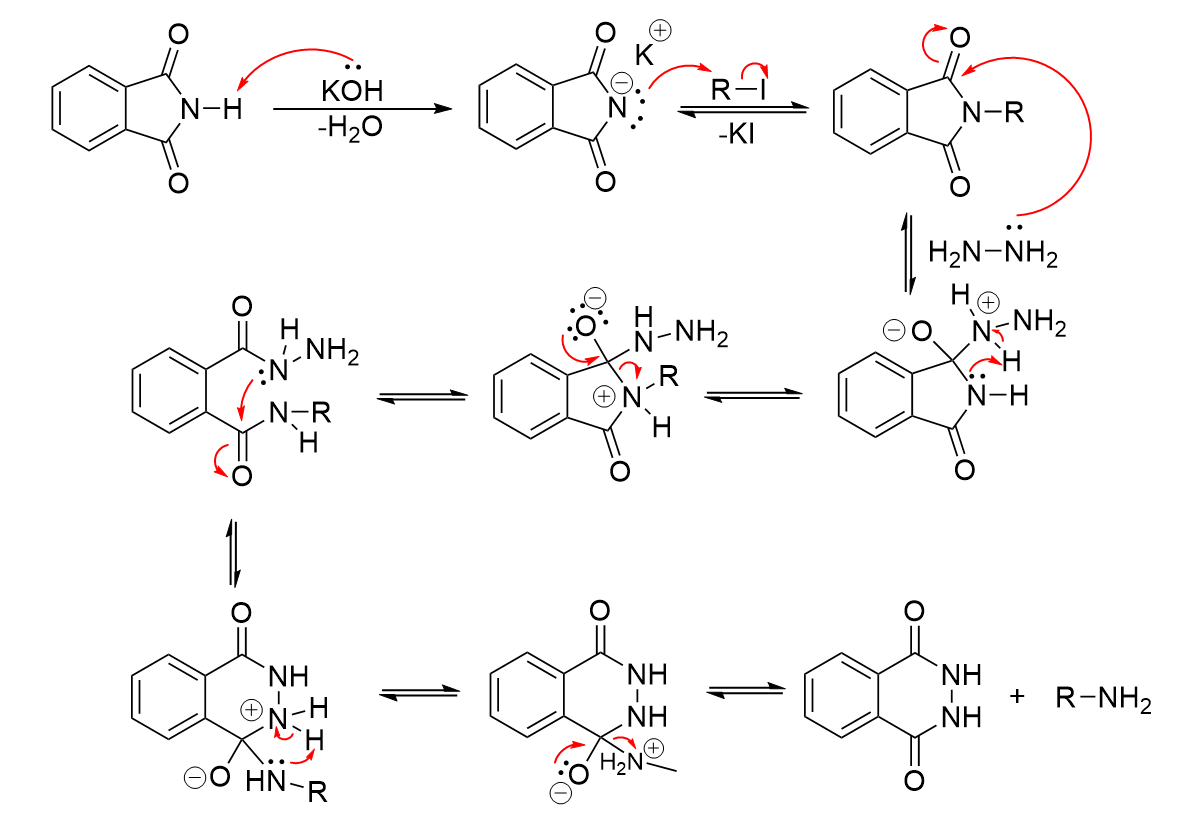
\includegraphics[width=0.8\linewidth]{Bilder/Hydrazinolyse Gabriel.png}
\end{figure}




\subsection{Orthoester}
\begin{figure}[H]
	\centering
	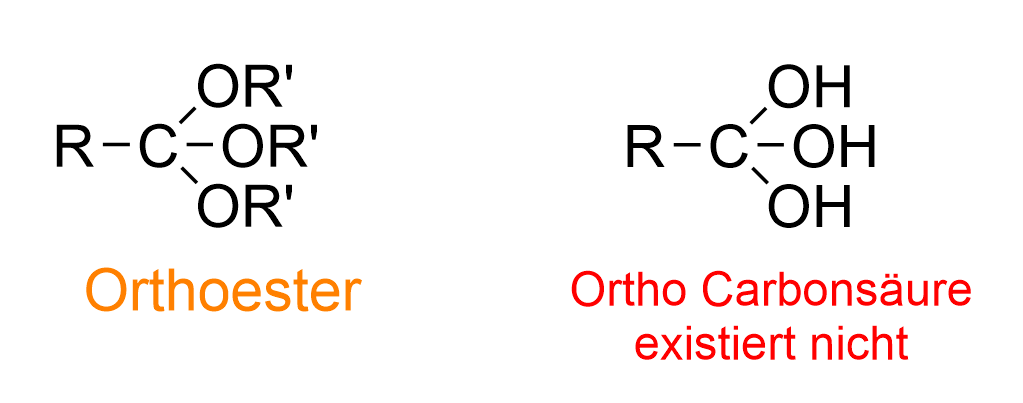
\includegraphics[width=0.5\linewidth]{Bilder/Orthoester.png}
\end{figure}

\subsubsection{Darstellungsmöglichkeiten}

\begin{enumerate}
	\item[a)] Williamsonsche Synthese
	\begin{equation}
		\ce{HCCl3 + 3NaOEt -> HC(OEt)3 + 3NaCl}
	\end{equation}
	\item[b)] aus Nitrilen 
	\begin{figure}[H]
	\centering
	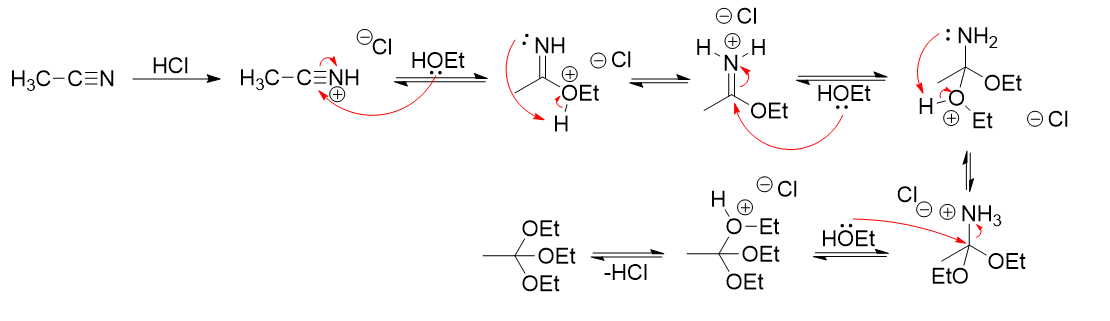
\includegraphics[width=1\linewidth]{Bilder/Orthoester aus Nitrilen.png}
	\end{figure}
\end{enumerate}


\subsection{Kohlensäurederivate}
\begin{figure}[H]
	\centering
	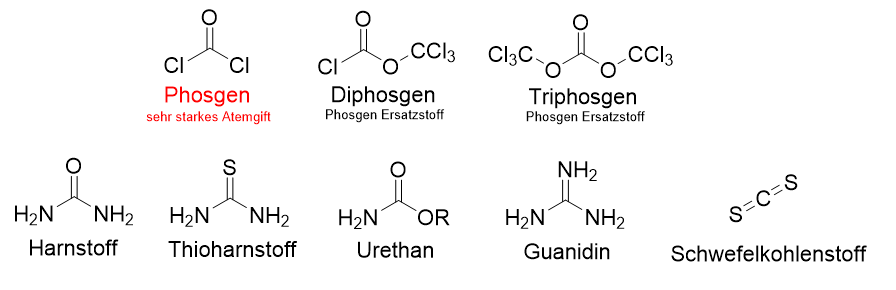
\includegraphics[width=1\linewidth]{Bilder/Kohlensäurederivate.png}
\end{figure}

\subsubsection{Darstellung von Phosgen}
\begin{equation*}
	\ce{CO + Cl2 ->[h\nu][oder 120 \si{\degreeCelsius}] COCl2}
\end{equation*}

\subsubsection{Reaktionen von Phosgen}
\begin{figure}[H]
	\centering
	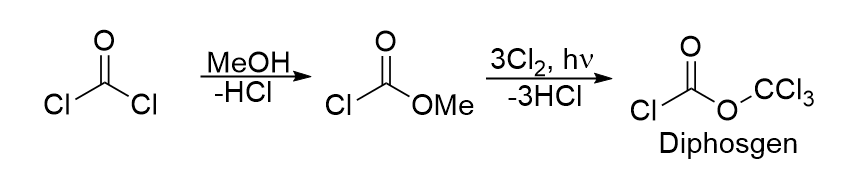
\includegraphics[width=0.75\linewidth]{Bilder/Diphosgen.png}
\end{figure}
Diese Reaktion kann auch mit doppelten Äquivalenten stattfinden und liefert dann das Triphosgen.

\subsection{Ketene}
\begin{figure}[H]
	\centering
	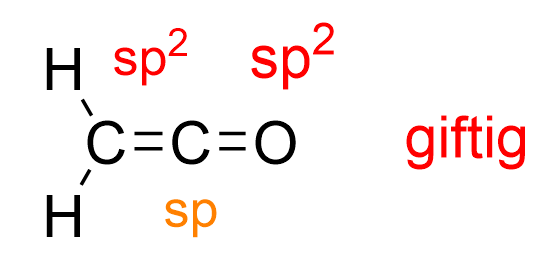
\includegraphics[width=0.3\linewidth]{Bilder/Keten.png}
\end{figure}

\subsubsection{Darstellung}
\begin{itemize}
	\item[a)] Pyrolyse von Ketonen
	\begin{figure}[H]
	\centering
	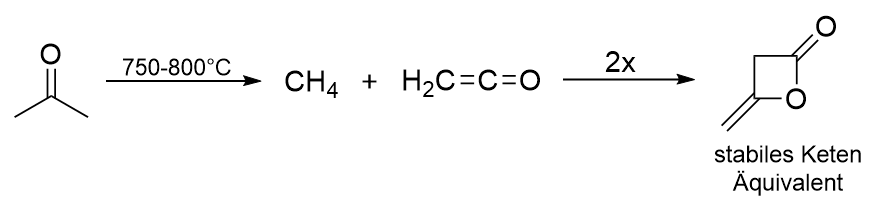
\includegraphics[width=0.8\linewidth]{Bilder/Pyrolyse von Ketonen.png}
\end{figure}
	\item[b)] aus Säurehalogeniden
\begin{figure}[H]
	\centering
	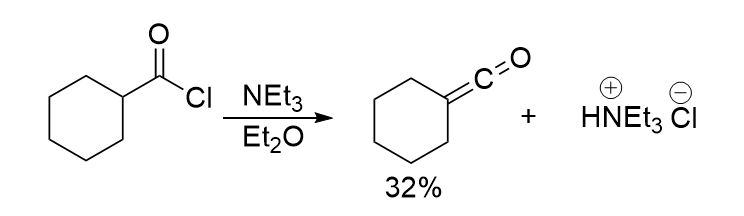
\includegraphics[width=0.7\linewidth]{Bilder/Keten aus Säurehalogeniden.png}
\end{figure}
	\item[c)] aus $\alpha$-Halogensäurebromiden
	\begin{figure}[H]
	\centering
	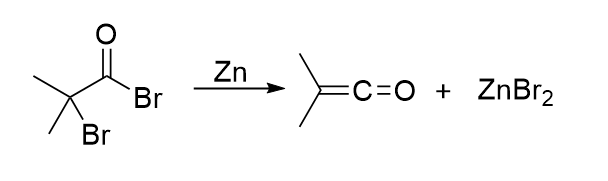
\includegraphics[width=0.65\linewidth]{Bilder/Ketene aus alpha-Halogensäurebromide.png}
\end{figure}
\end{itemize}

\subsubsection{Reaktionen von Ketenen}
Ketene reagieren als Superanhydride.
\subsubsection*{Reaktion mit Wasser}
\begin{figure}[H]
	\centering
	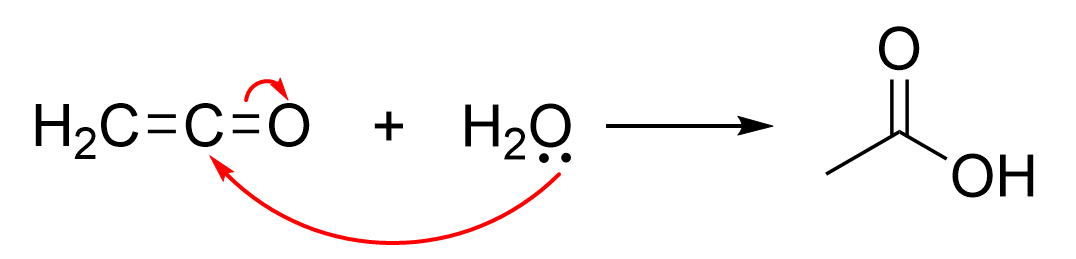
\includegraphics[width=0.5\linewidth]{Bilder/Keten mit Wasser.png}
\end{figure}

\subsubsection*{Reaktion mit Anilin}
\begin{figure}[H]
	\centering
	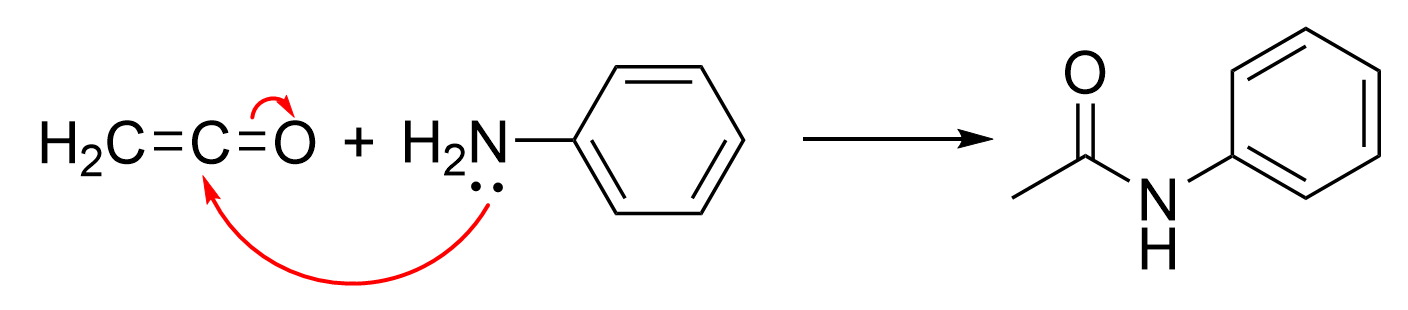
\includegraphics[width=0.65\linewidth]{Bilder/Ketene mit Anilin.png}
\end{figure}


\subsection{Reaktionen von Carbonsäurederivaten}
\begin{figure}[H]
	\centering
	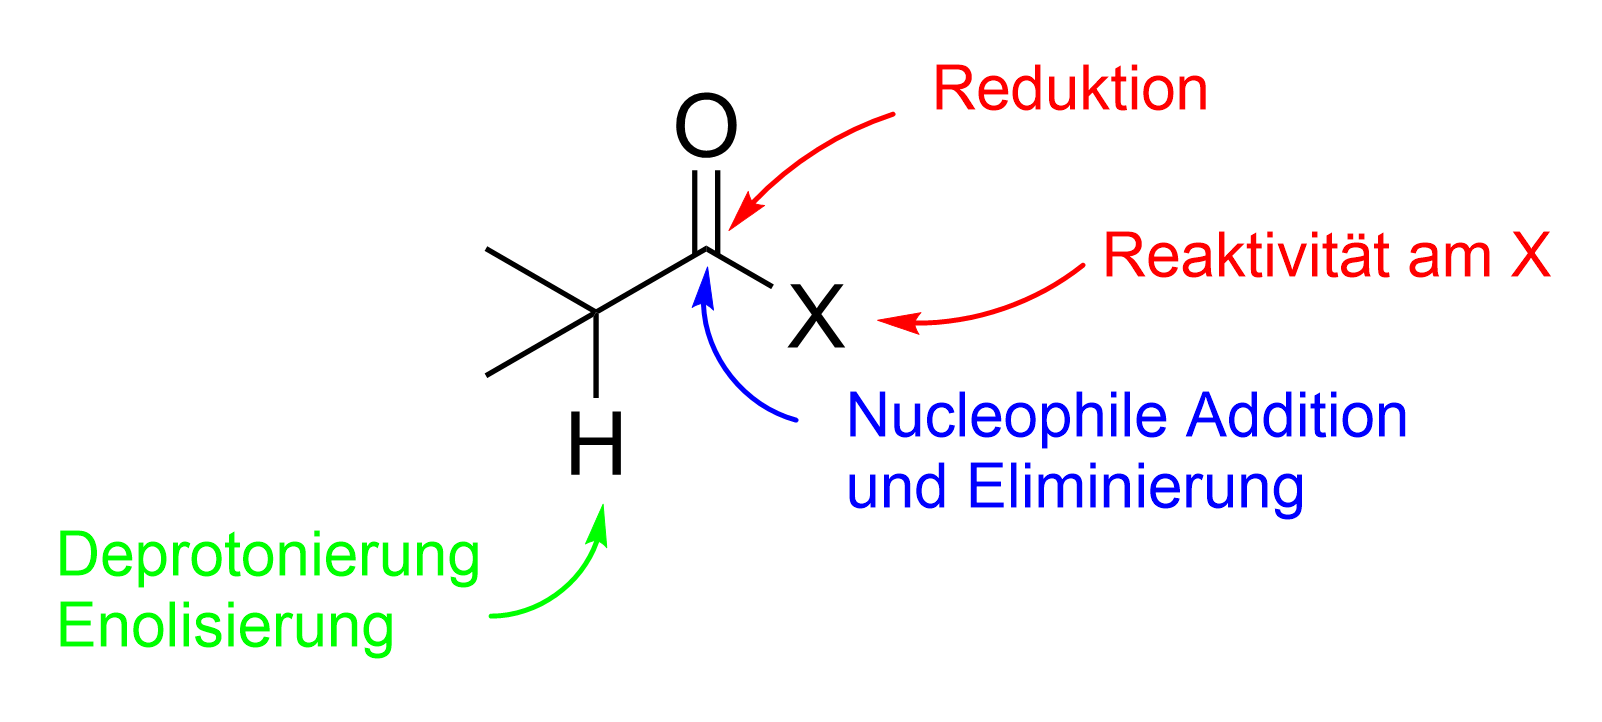
\includegraphics[width=0.6\linewidth]{Bilder/Übersicht Reaktionen von Carbonsäure-Derivaten.png}
\end{figure}
Als Faustregel gilt, dass umso negativer die Abgangsgruppe X ist, desto bessere Acylierungsmittel sind die Carbonsäurederivate.
Eine Ausnahme sind Thioester, welche Reaktiver sind als Ester. Der Grund hierfür ist die geringe Mesomeriestabilisierung des Thioesters, da Schwefel ein größeres Atom ist als Sauerstoff und dadurch eine schlechte orbitalüberlappung zustandekommt.
\subsubsection{Reduktionen}
\subsubsection*{Einelektronen Reduktionen}
Sowohl die Bouveault Blanc Reduktion als auch die Acyloin Kondensation können auch Intramolekular stattfinden um Cyclen zu bilden.
Die Bouveault Blanc Reduktion findet in protischen Lösemitteln statt und die Acyloin-Kondensation in aprotischen Lösemitteln.
\begin{enumerate}
	\item Bouveault-Blanc-Reduktion
	\begin{figure}[H]
	\centering
	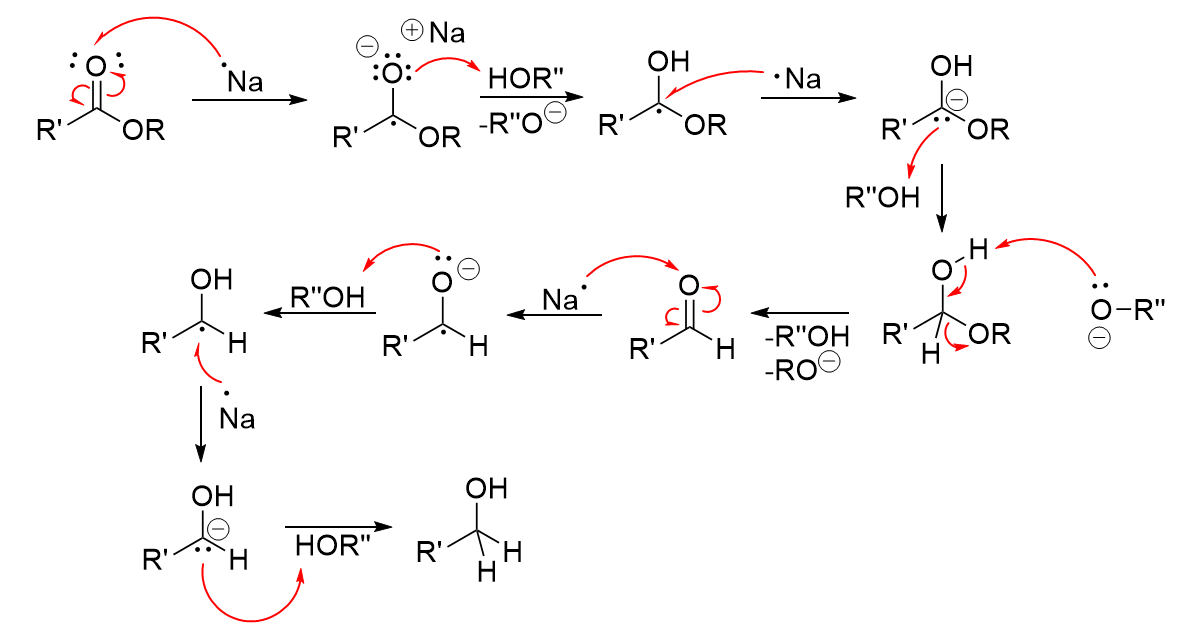
\includegraphics[width=0.9\linewidth]{Bilder/Bouveault Blanc Reaktion.png}
	\end{figure}
	\item Acyloin-Kondensation
	\begin{figure}[H]
	%\centering
	\hspace{1cm}
	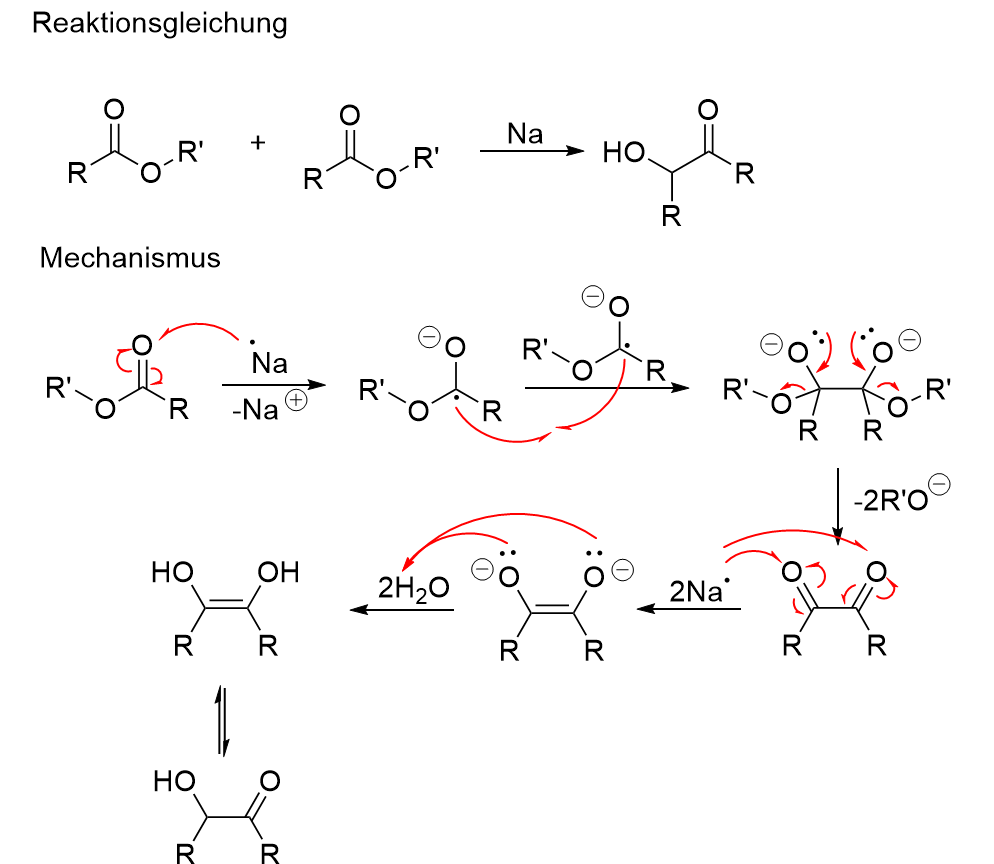
\includegraphics[width=0.7\linewidth]{Bilder/Acyloin-Kondensation.png}
	\end{figure}

\end{enumerate}

\subsubsection*{Reduktion mit komplexen Hydriden}
\begin{figure}[H]
	\centering
	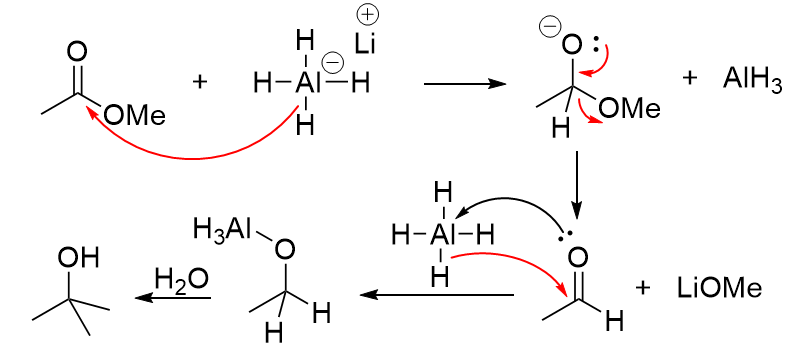
\includegraphics[width=0.55\linewidth]{Bilder/LiAlH4.png}
\end{figure}
Dieser Hydrid-Transfer ist Analog bei DIBAL (Diisobutylaluminiumhydrid), jedoch ist bei DIBAL bei tiefen Temperaturen die isolierung des Aldehyds möglich, während \ce{LiAlH4} bis zum Alkohol direkt Reduziert. 
\begin{figure}[H]
	\centering
	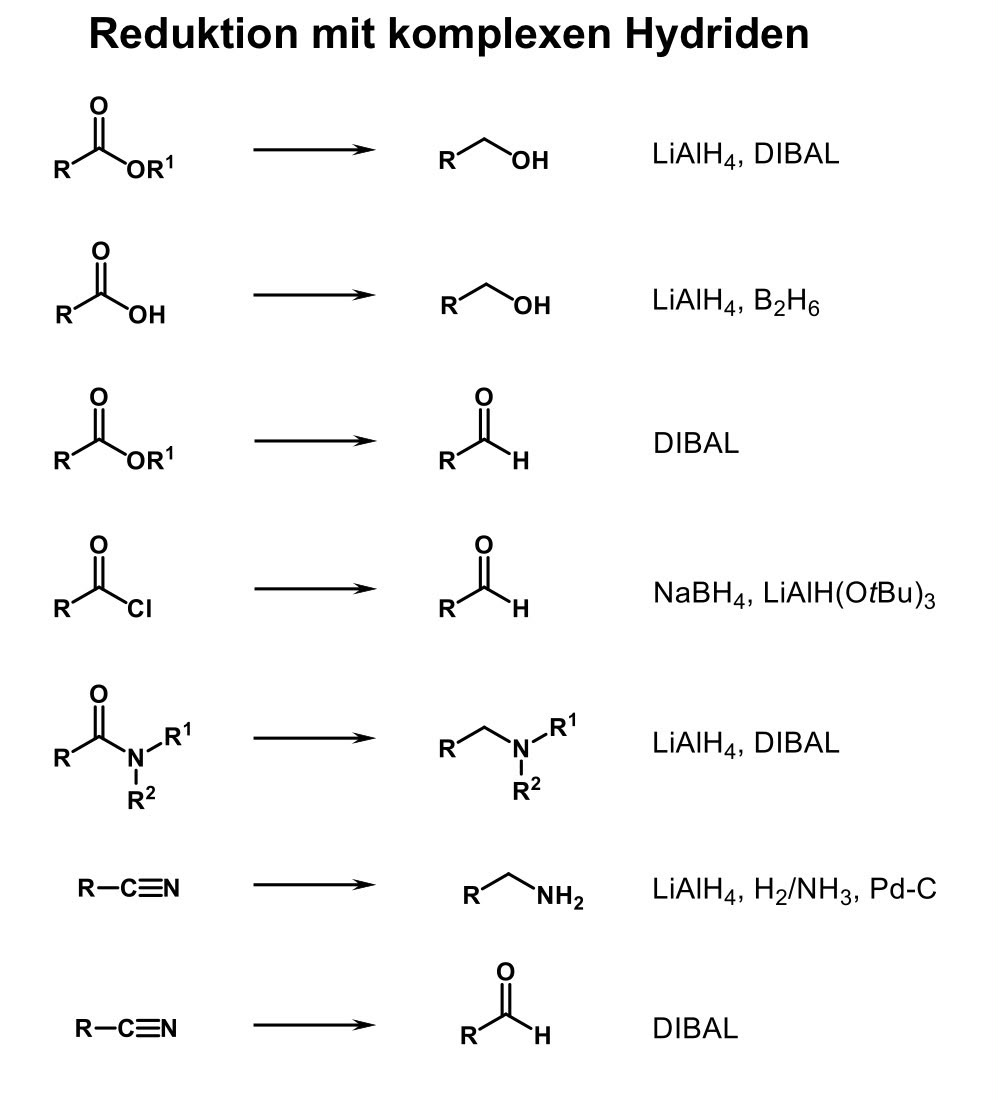
\includegraphics[width=0.6\linewidth]{Bilder/Reduktion mit komplexen Hydriden.jpeg}
\end{figure}

\section{Nitrile}
\subsection{Stoffchemie}
\begin{figure}[H]
	\centering
	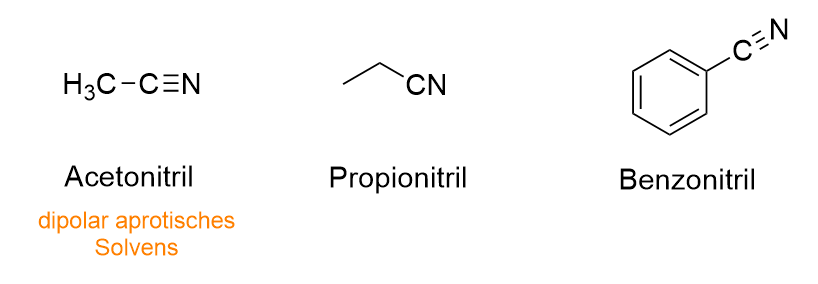
\includegraphics[width=0.7\linewidth]{Bilder/Nitrile Stoffchemie.png}
\end{figure}

\subsection{Darstellung von Nitrilen durch \ce{S_N}}
\begin{figure}[H]
	\centering
	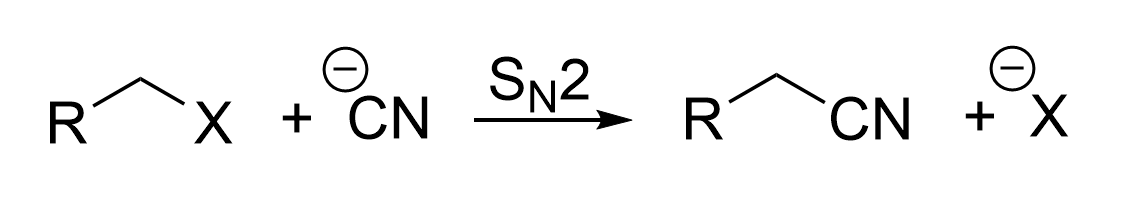
\includegraphics[width=0.5\linewidth]{Bilder/Nitrile durch SN.png}
\end{figure}

\subsection{Darstellung von Nitrilen aus Säureanhydriden}
\begin{figure}[H]
	\centering
	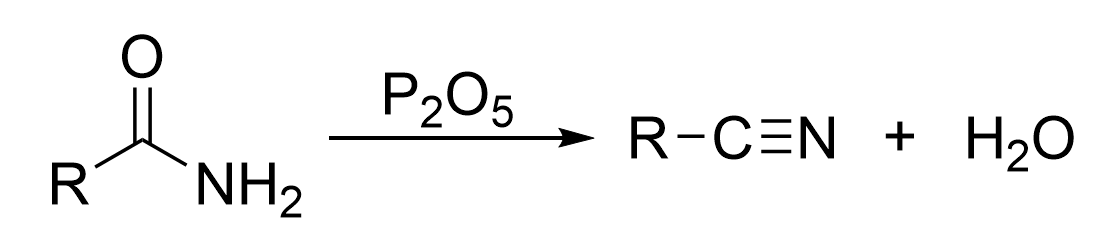
\includegraphics[width=0.5\linewidth]{Bilder/Nitrile aus Amiden.png}
\end{figure}


\newpage
\section{Aminosäuren, Peptide}
Als Bausteine in Proteinen kommen nur $\alpha$-Aminosäuren vor. Es gibt genau 20 proteinogene Aminosäuren, wovon 8 Aminosäuren essentiell sind und damit über die Nahrung aufgenommen werden müssen.
Nicht proteinogene Aminosäuren kommen nur im Stoffwechsel vor, hier finden sich auch $\beta$ und $\gamma$-Aminosäuren.
\begin{figure}[H]
	\centering
	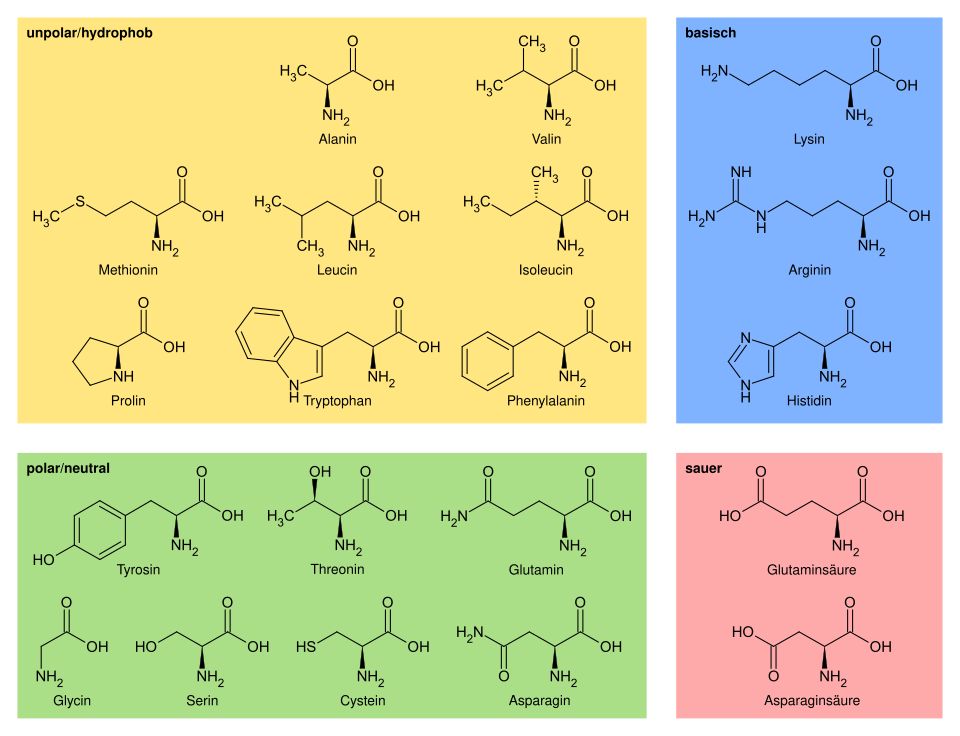
\includegraphics[width=1\linewidth]{Bilder/Aminosäuren.png}
\end{figure}
\noindent Die Konfigurationen D/L und R/S sind unabhängig voneinander und lassen sich nicht ineinander übersetzen.\\

\noindent Aminosäuren liegen als Zwitterion vor und sind dadurch gut Waserlöslich. Zudem sind sie Amphoter, da sie gleichzeitig Säure und Base Funktionen besitzen.\\

\noindent Bei der Titration von Aminosäuren gibt es den Isoelektrischen Punkt. Dies ist der Äquivalenzpunkt der Titration und die Aminosäure liegt als Zwitterion vor, es liegen also gleich viele kationische wie anionische Gruppen vor. Oberhalb bzw unterhalb der pKs-Werte der Aminosäure liegt die Aminosäure entweder als Anion oder Kation vor, da hier entweder nur die Amino oder die Carbonsäure-Gruppe protoniert oder deprotoniert vorliegt. Der Isoelektrische Punkt entspricht nicht dem neutralpunkt (pH=7)!
Für den Isoelektrischen Punkt (IEP) gilt 
\[
pH_\mathrm{IEP}=\frac{pK_S(I)+pK_S(II)}{2}
\]
\begin{figure}[H]
	\centering
	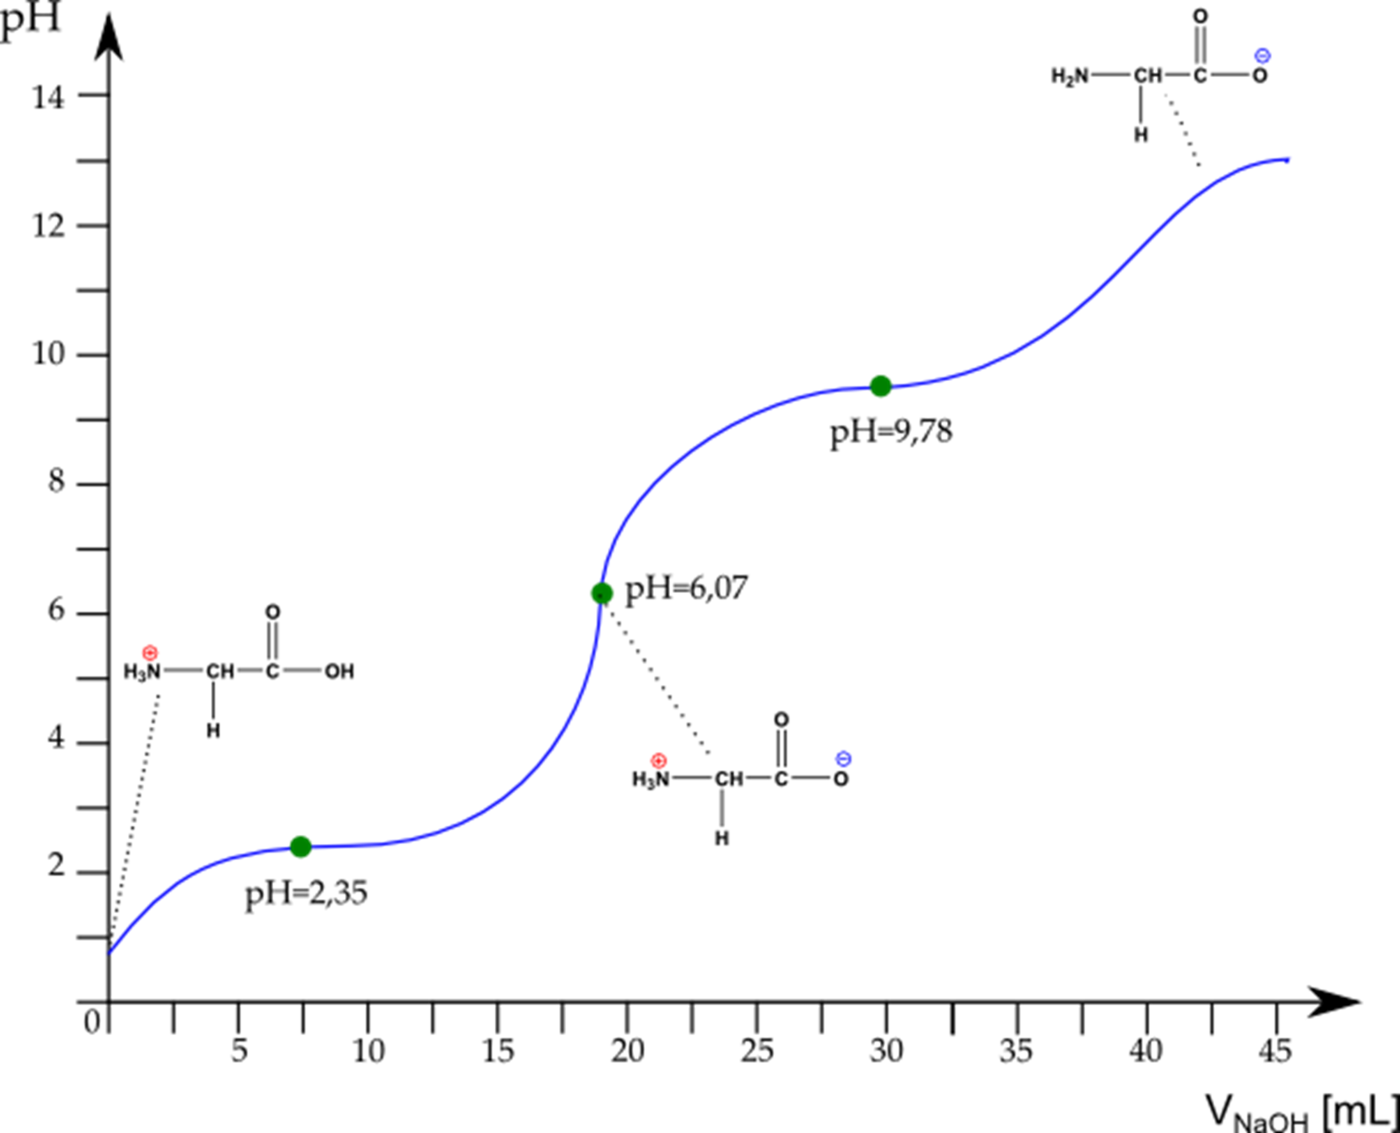
\includegraphics[width=1\linewidth]{Bilder/titrationskurve alanin.png}
	\caption{Titrationskurve der neutralen Aminosäure Glycin.}
\end{figure}
\begin{figure}[H]
	\centering
	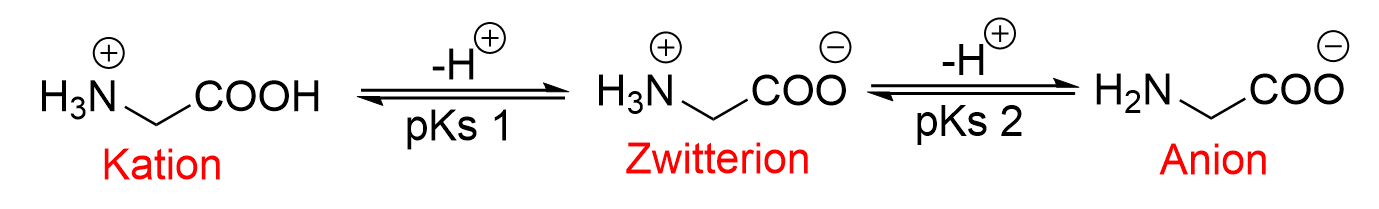
\includegraphics[width=1\linewidth]{Bilder/titration glycin.png}
\end{figure}
Aminosäuren mit weiteren protonierbaren oder deprotonierbaren Seitenketten weisen mehr als zwei pKs-Werte auf. 

\subsection{Elektrophorese}
Die Elektrophorese ist eine Methode zur Trennung von Aminosäuren/Proteinen mittels Hochspannung und ihrem Isoelektrischen Punkt. Der pH-Wert der Elektrophorese entscheidet, welche Ladung die Aminosäure besitzt. Somit liegt die eine Aminosäure bei dem gewählten pH-Wert als Kation vor und eine andere Aminosäure als Anion und eine andere liegt als Zwitterion vor, da der pH-Wert dem IEP entspricht. Die Kationische Form bewegt sich nun in Richtung der negativ geladenen Elektrode und die Anionische Form zur positiv geladenen Elektrode. Die Aminosäure am IEP bewegt sich nicht, da sie nach außen hin Ladungstechnisch neutral ist. Als Stationäre Phase wird Gel oder Papier verwendet. Für die Wanderung spielt ebenso die Größe bzw Molmasse der Aminosäuren/Proteine eine Rolle.


\subsection{Diketopiperazin-Bildung}
Der freie Glycinethylester ist instabil und cyclisiert zum Diketopiperazin, einem cyclischen Peptid. Daher wird für den Glycinethylester das stabile Hydrochlorid verwendet.
\begin{figure}[H]
	\centering
	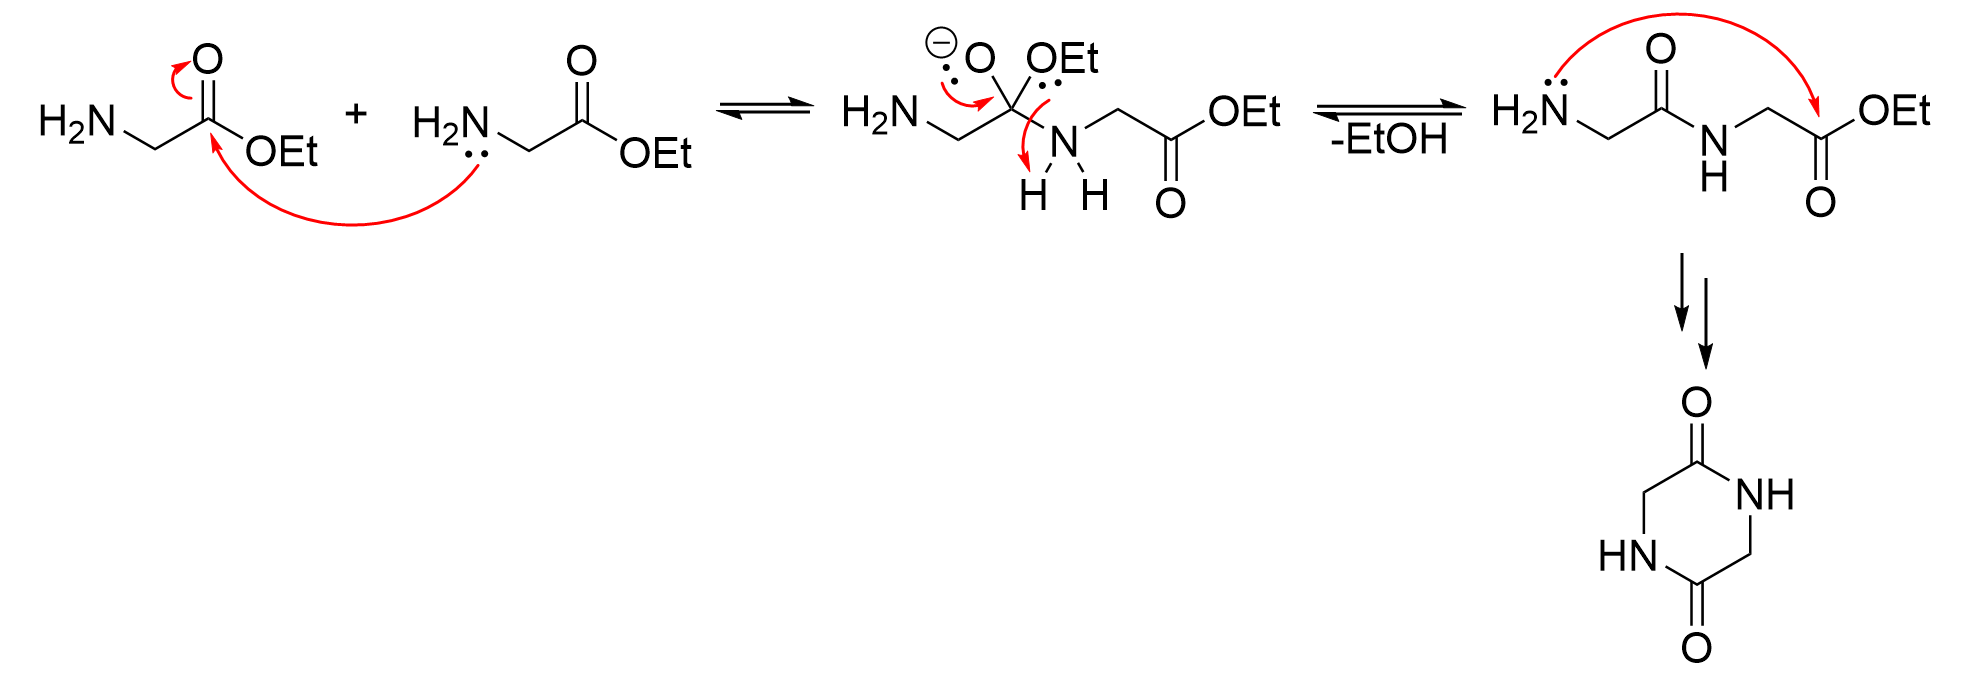
\includegraphics[width=1\linewidth]{Bilder/Diketopiperazin.png}
\end{figure}




\subsection{Darstellung von Aminosäuren}
\subsubsection{Strecker-Synthese}
\begin{figure}[H]
	\centering
	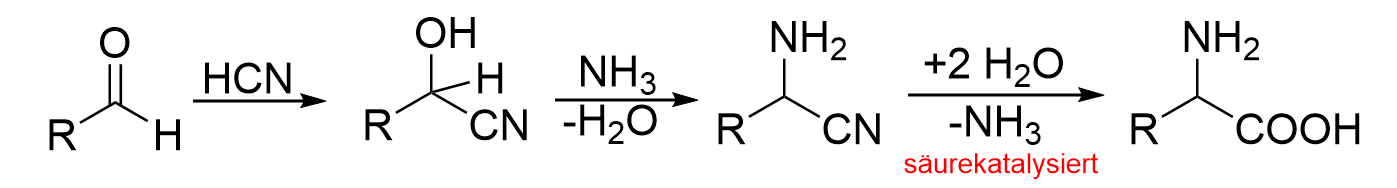
\includegraphics[width=0.9\linewidth]{Bilder/Strecker-Synthese.png}
\end{figure}

\subsubsection{Nucleophile Substitution}
\begin{figure}[H]
	\centering
	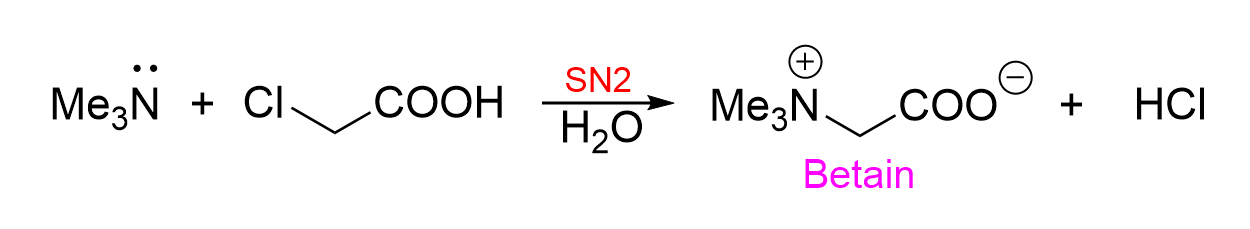
\includegraphics[width=0.9\linewidth]{Bilder/SN2 AS Darstellung.png}
\end{figure}


\subsubsection{Beckmann-Umlagerung}
\begin{figure}[H]
	\centering
	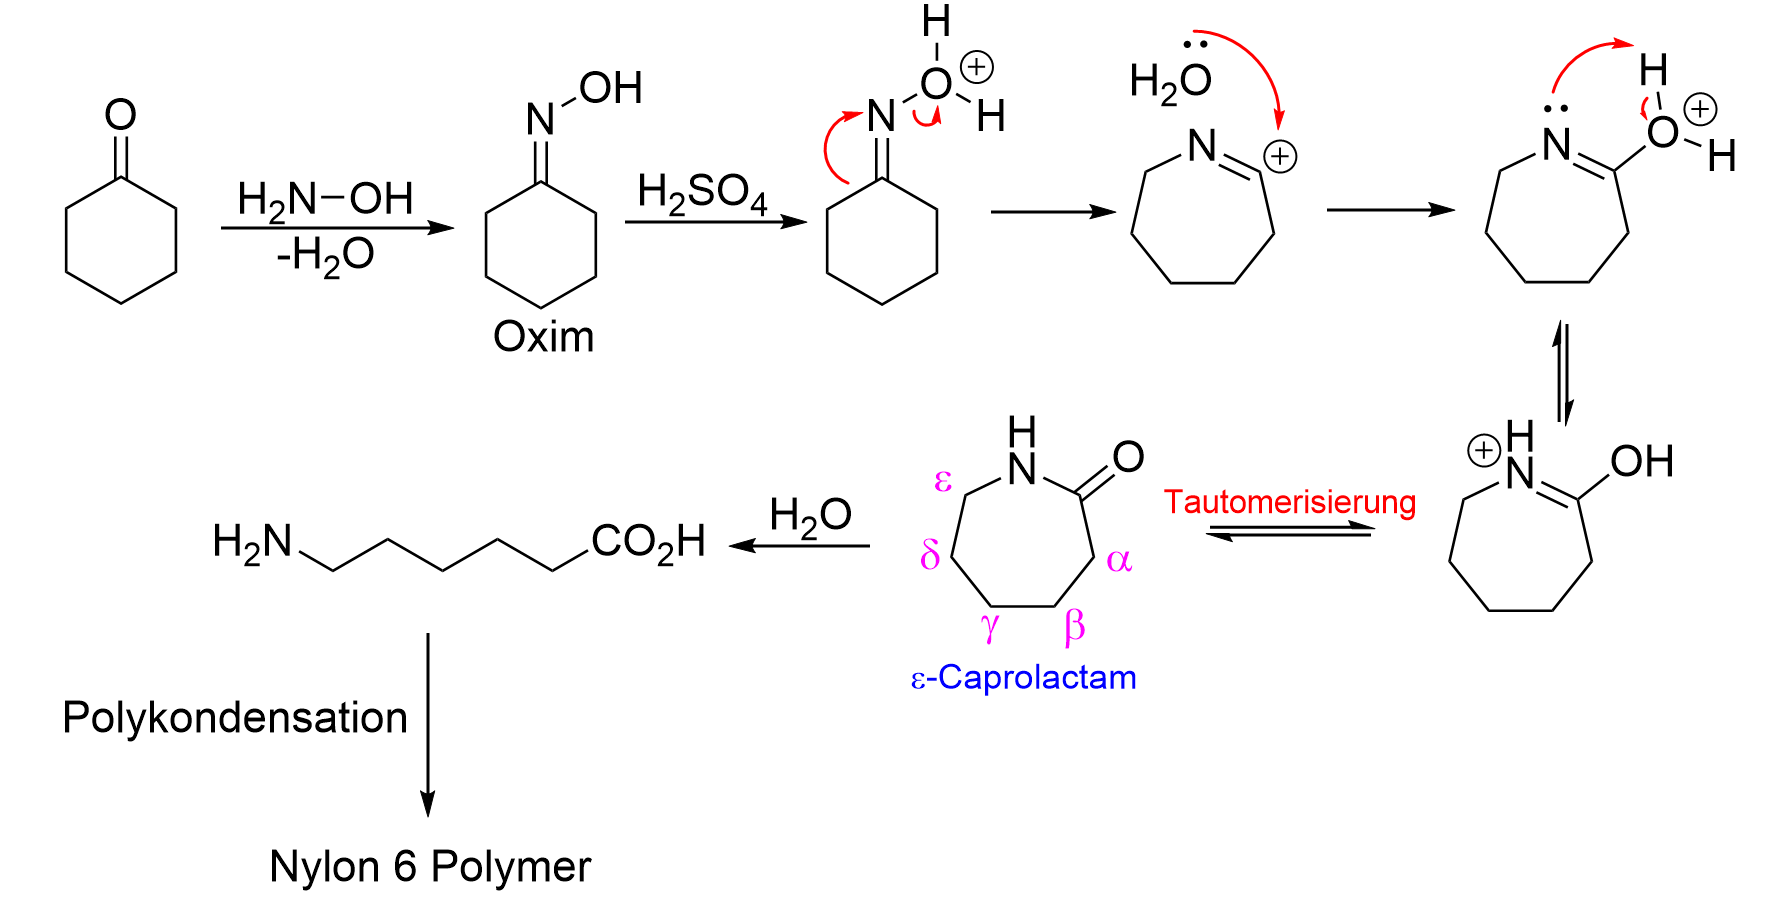
\includegraphics[width=1\linewidth]{Bilder/Beckmann-Umlagerung+Poly.png}
\end{figure}

\subsection{Reaktionen}
\subsubsection{Amidbildung}
\begin{figure}[H]
	\centering
	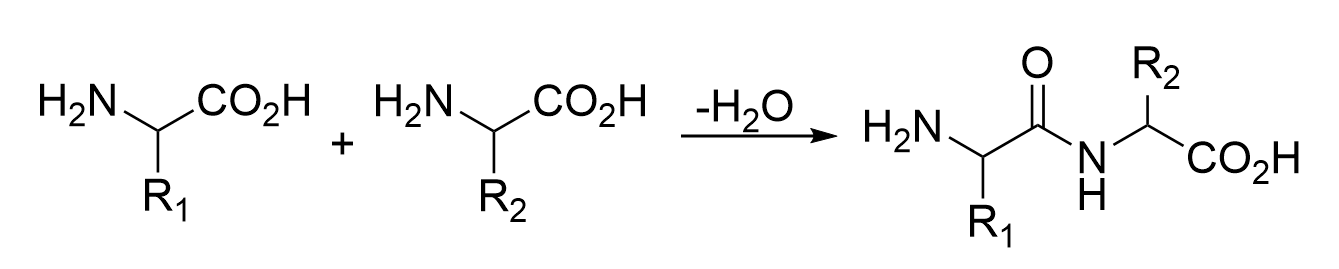
\includegraphics[width=0.9\linewidth]{Bilder/Amidbildung-v2.png}
\end{figure}

\subsubsection{Reaktionen zum analytischen Nachweiß}
\subsubsection*{Sörensen-Titration}
Aminosäuren sind gut titrierbar nach Schützen der Aminogruppe.
\begin{figure}[H]
	\centering
	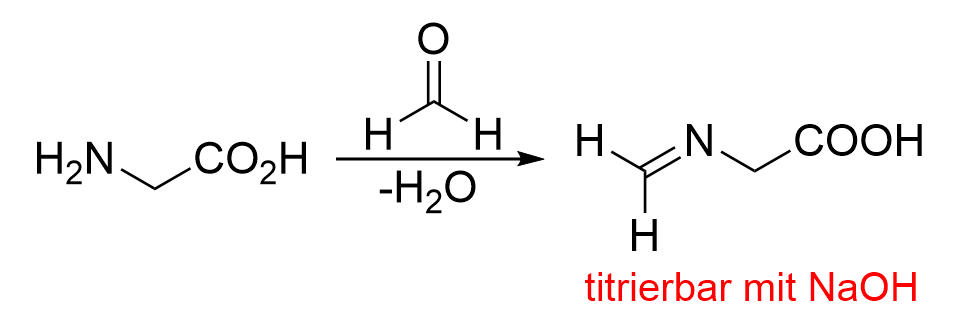
\includegraphics[width=0.7\linewidth]{Bilder/Sörensen-Titration.png}
\end{figure}


\subsubsection*{Kupfer-Komplexe}
Aminosäuren bilden intensiv blaue Kupfer-Komplexe. Diese Kupfer-Komplexe können auch zur Reinigung von Aminosäuren und als Schutzgruppe eingesetzt werden.
\begin{figure}[H]
	\centering
	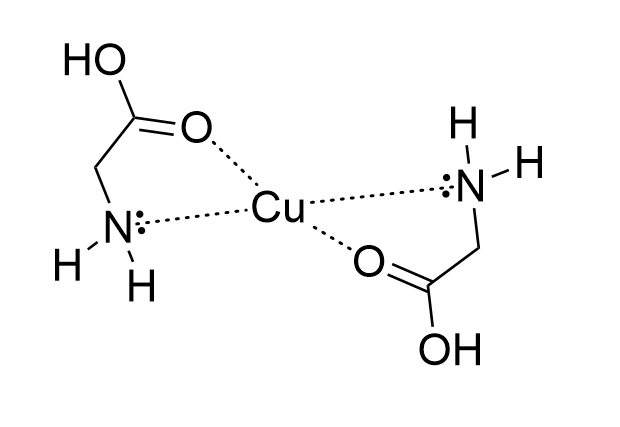
\includegraphics[width=0.4\linewidth]{Bilder/Kupfer-Komplex-AS.png}
\end{figure}


\subsubsection*{Ninhydrin-Reaktion}
\begin{figure}[H]
	\centering
	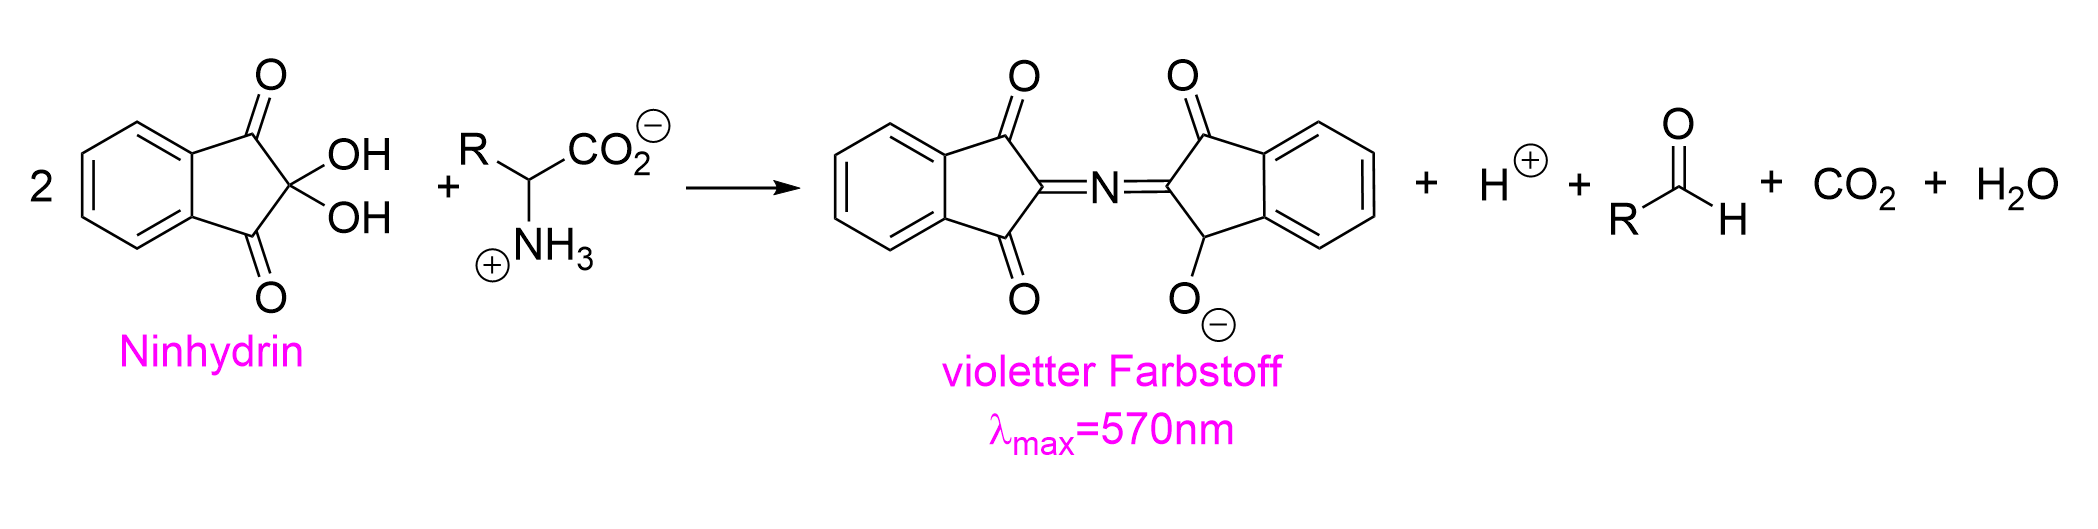
\includegraphics[width=1\linewidth]{Bilder/Ninhydrin.png}
\end{figure}
\subsubsection*{Mechanismus der Ninhydrin Reaktion}
\begin{figure}[H]
	\centering
	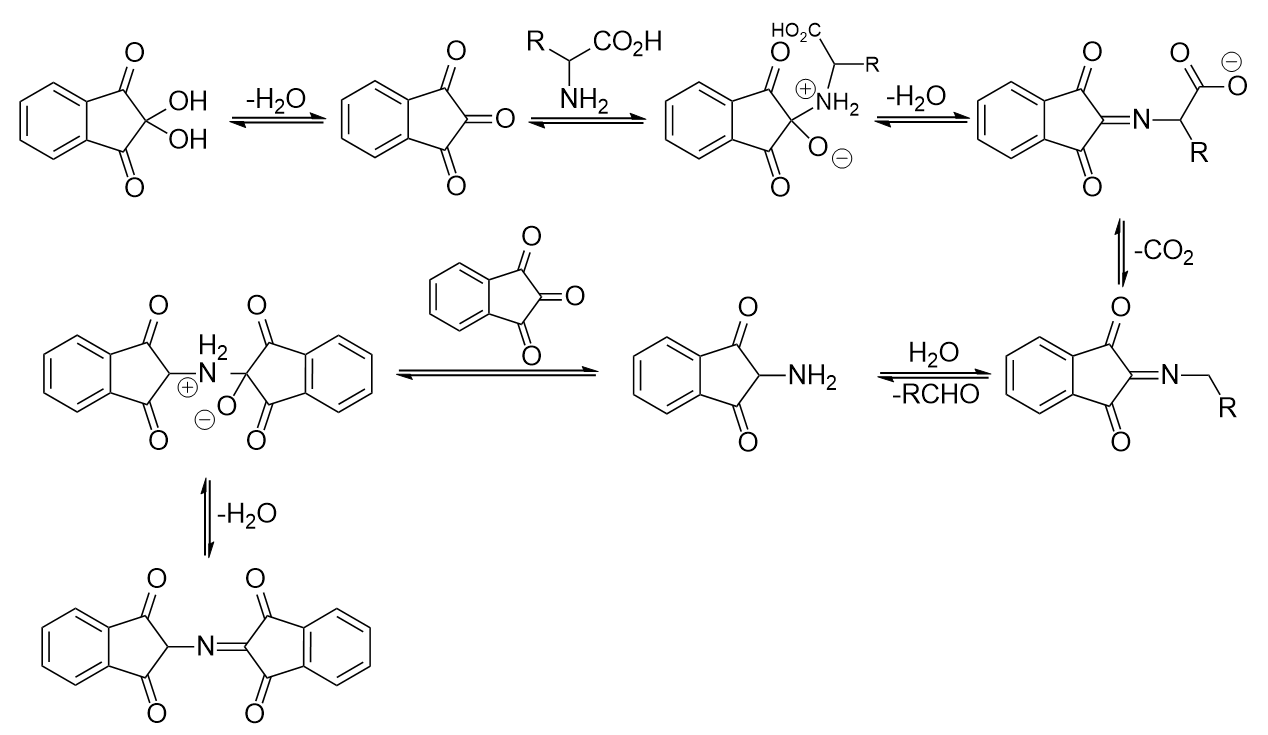
\includegraphics[width=1\linewidth]{Bilder/Ninhydrin-Mechanismus.png}
\end{figure}


\subsection{Peptide}
Peptide entstehen durch Säureamidartige Verknüpfung von Aminosäuren (Peptidbindung). Aufgrund der Mesomeriestabilisierung (partieller Doppelbindungscharakter von C-N) ist die Rotation um die CN-Bindung erschwert.
\begin{figure}[H]
	\centering
	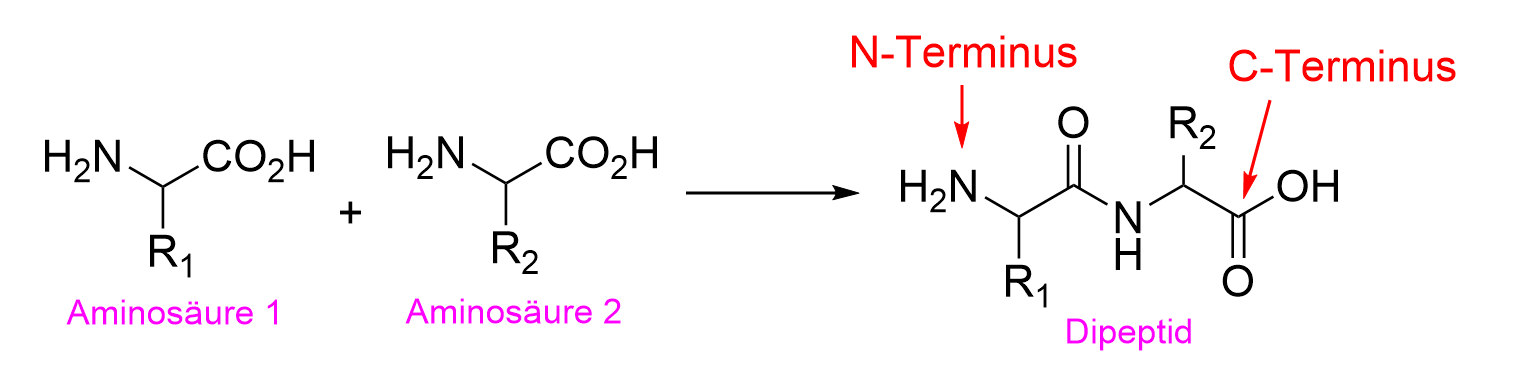
\includegraphics[width=1\linewidth]{Bilder/Dipeptid.png}
\end{figure}
Ein prominentes Dipeptid ist Aspartam, bestehend aus L-Asparagin und L-Phenylalaninmethylester
\subsubsection{Polypeptide}
Bei Polypeptiden ist die Hauptkette immer gleich, aber die Seitenketten R1, R2, R3, \ldots bestimmen die Struktur, das chemische Verhalten und die biologische Aktivität.

\subsection{Proteine}
Proteine sind Polypeptide mit einer 3D-Struktur. Diese setzt sich aus folgenden Elementen zusammen:
\begin{enumerate}
	\item[a)] \textbf{Primärstruktur:}\\
	Die Primärstruktur stellt die einfache Aminosäuresequenz dar.
	\item[b)] \textbf{Sekundärstruktur:} \\
	Die Sekundärstruktur entsteht durch die Ausbildung von H-Brücken. Es gibt zwei Sekundärstrukturen, einmal $\alpha$-Helix und einmal $\beta$-Faltblatt. Die Alpha-Helix beschreibt die Konformation einer Peptidkette, welche durch intramolekulare H-Brücken entsteht. Die Beta-Faltblatt sind paralelle oder antiparallele H-brücken zwischen zwei Peptidketten.
	\begin{figure}[H]
	\centering
	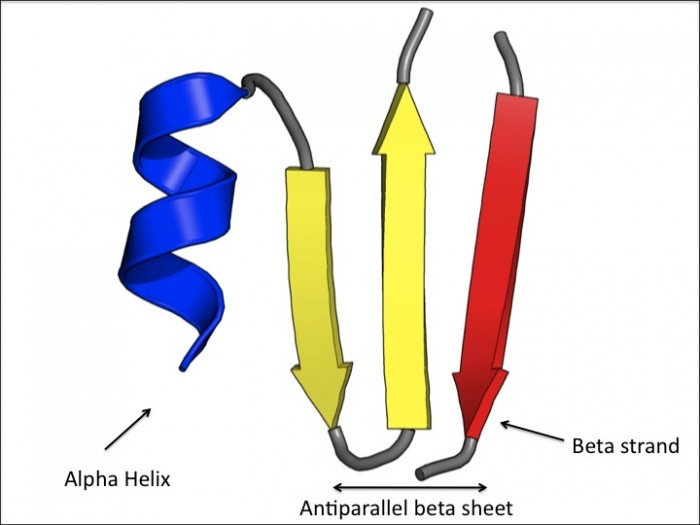
\includegraphics[width=0.7\linewidth]{Bilder/sekundärstruktur.png}
	\end{figure}
	Ist Prolin in der Peptidkette eingebaut, so unterbricht diese Aminosäure die regelmäßigen alpha und beta Einheiten und führt zu sogenannten $\beta$-Turns (Faltungen der Peptidkette). Diese Beta-Turns verbinden die Beta-Faltblatt Strukturen.
	\begin{figure}[H]
	\centering
	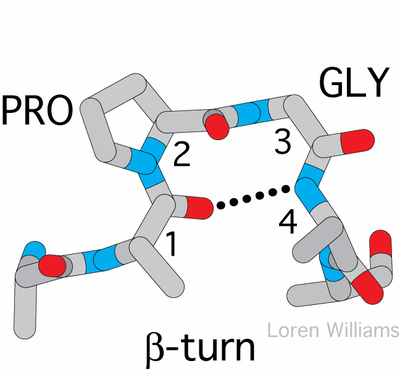
\includegraphics[width=0.5\linewidth]{Bilder/Beta-Turn.png}
	\end{figure}
	\item \textbf{Tertiärstruktur}\\
	Die Tertiärstruktur kommt durch räumliche Anordnung der Helices und Faltblätter durch Disulfidbrücken zustande.
	\item \textbf{Quartiärstruktur}\\
	Unter der Quartiärstruktur werden komplexe Proteine verstanden. Sie sind meist aus mehreren Proteinen zusammengelagert, die sich um ein Metallatom oder Nichtprotein zusammenlagern. Es handelt sich also um Aggregate von Proteinen. Beispiel ist Hämoglobin, welches aus vier Untereinheiten besteht. Jede Untereinheit bindet ein Molekül \ce{O2}. Die Bindung des ersten Moleküls Sauerstoff erhöht die Affinität zur Bindung des nächsten. Dies bezeichnet man als Kooperativen Effekt.
\end{enumerate}

\subsubsection{Chemische eigenschaften von Proteinen}
%Ich habe ehrlich gesagt keine Ahnung was ich da hinschreiben soll. Wir haben da nur Experimente zu aufgeschrieben.


\subsubsection{Biologische Funktionen der Proteine}
Biologische Funktionen der Proteine sind
\begin{itemize}
	\item Biokatalysatoren: Enzyme
	\item Transportmoleküle: Serumalbumine, Hämoglobin (\ce{O2}-Transport)
	\item Strukturgebende Moleküle: Collagen (Bindegewebe), Keratin (Haare)
	\item Strukturerkennende Moleküle: Rezeptoren, Hormone (Insulin)
	\item Abwehr: Blutgerinnung, Antikörper 
	\item Pufferung: Hämoglobin 
	\item Wasserbindung 
	\item Energiespeicher 
\end{itemize}
Wichtige natürliche Peptide sind z.B das Bradykinin, welches im Blutplasma vorkommt und an der Regulation des Blutdrucks beteiligt ist. Andere wichtige natürliche Peptide sind Substanz P, welche im Gehirn als Neurotransmitter vorkommt und an der Übertragung von Schmerzsignalen beteiligt ist, sowie Vasopressin, welches ein Hormon aus dem Hypophysenlappen ist, welches in den Blutkreislauf geht und für die Regulation der Wasserauscheidung durch die Nieren verantwortlich ist. Dadurch beeinflusst es den Blutdruck. Ein Mangel an Vasopressin führt zu Diabetes insipidus.

\subsubsection{Peptid-Analyse}
\subsubsection*{Markierung N-Terminaler Aminosäuren mit Sanga's Reagenz}
\begin{figure}[H]
	\centering
	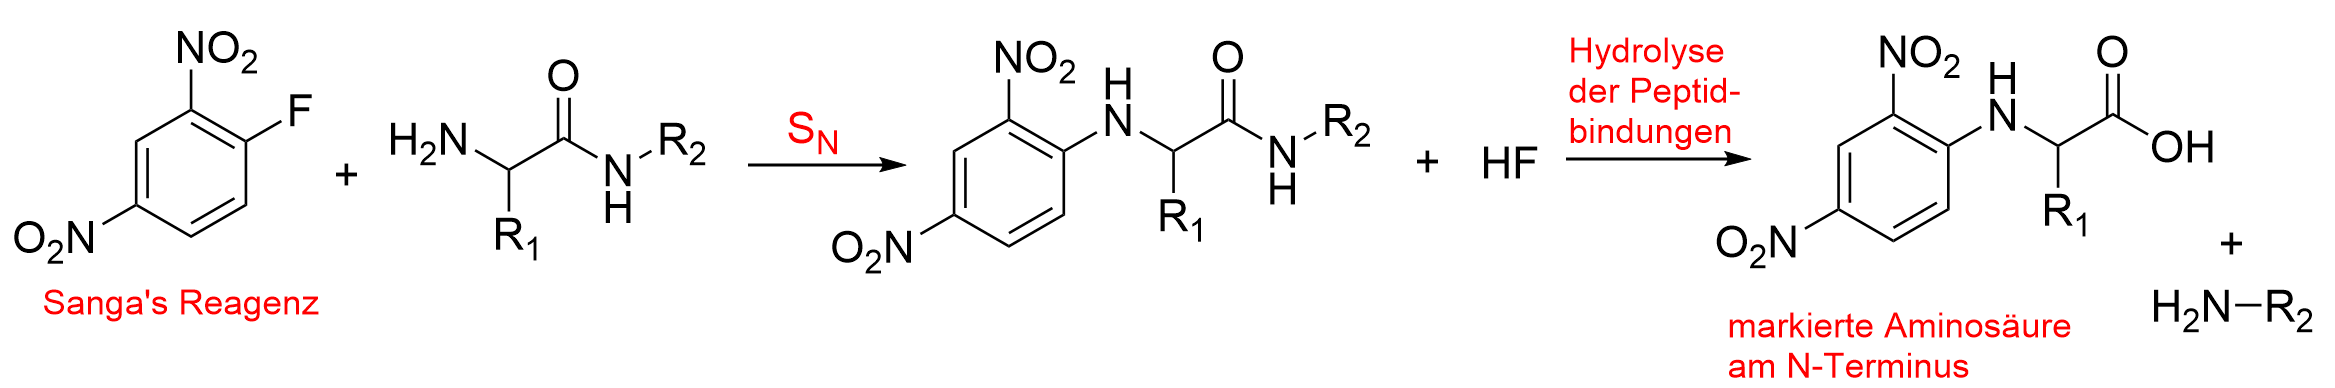
\includegraphics[width=1\linewidth]{Bilder/Sanga.png}
\end{figure}


\subsubsection*{Edman-Abbau}
Der Edman-Abbau bist ein sukzessiver Abbau der Peptidkette vom N-Terminus aus.
\begin{figure}[H]
	\centering
	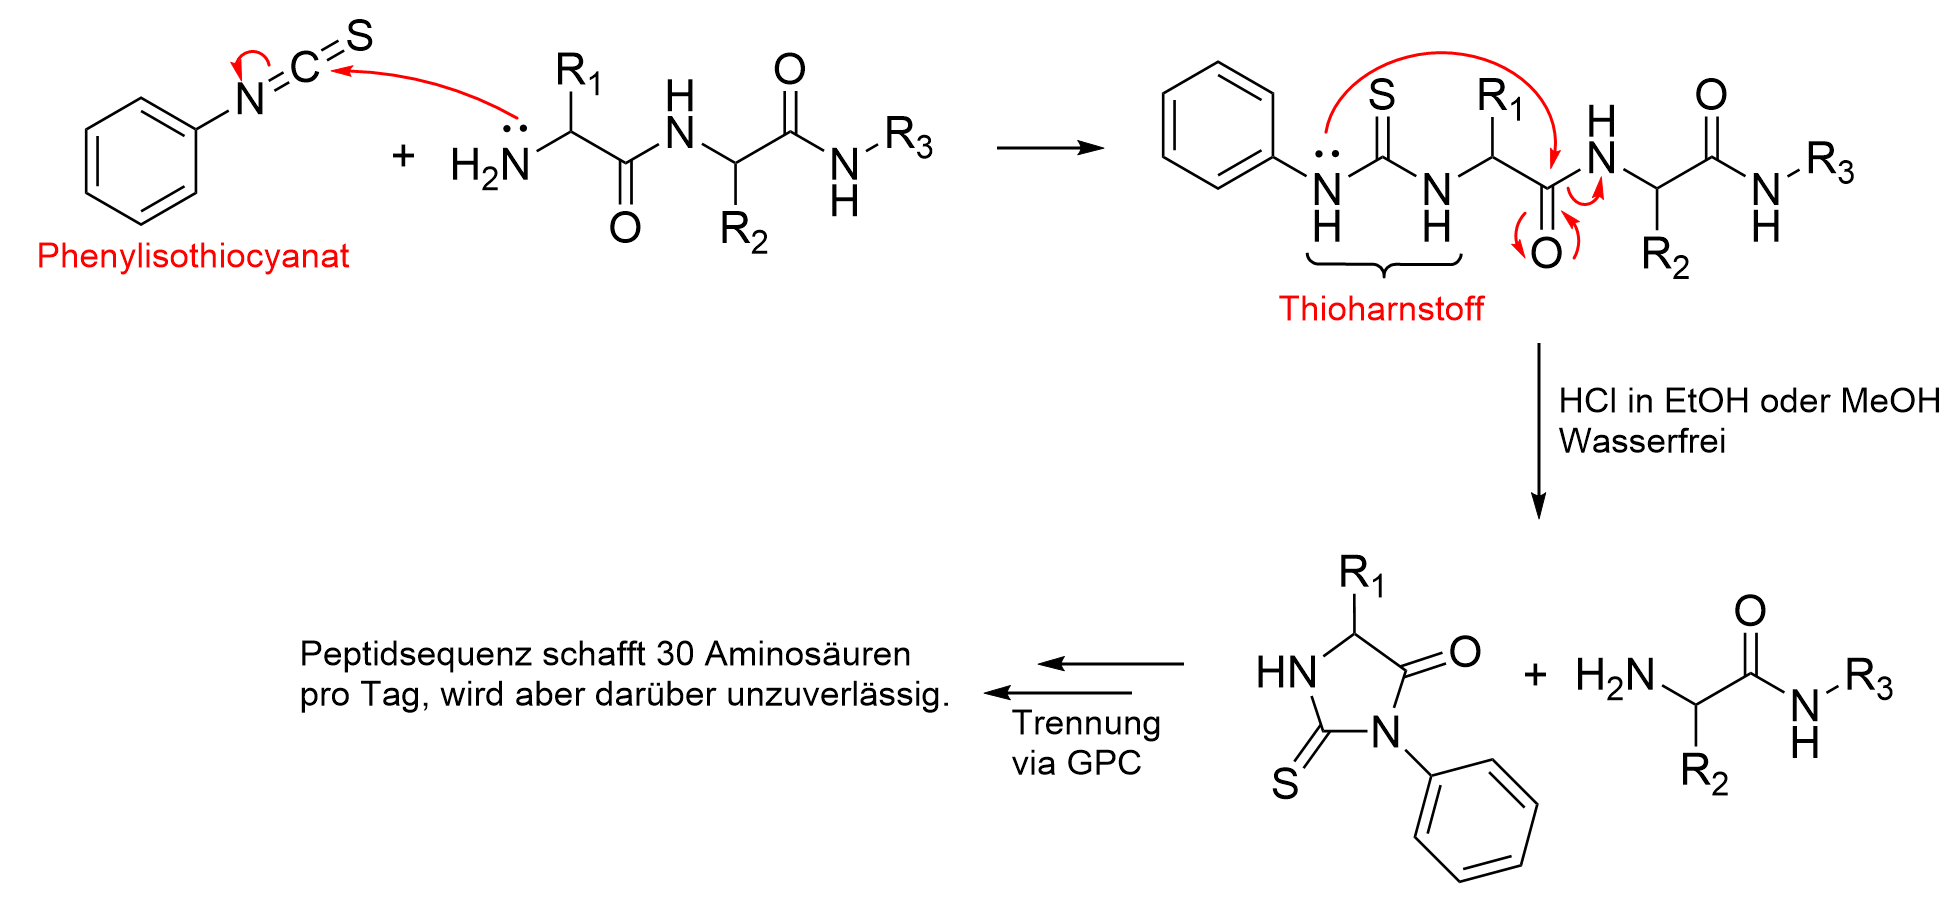
\includegraphics[width=1\linewidth]{Bilder/Edman-Abbau.png}
\end{figure}



\subsubsection{Peptid Synthese}
\subsubsection*{Peptid Synthese in Lösung}
Bei der Peptid-Synthese in Lösung müssen Schutzgruppen für das Amin, die Carbonsäure und die Seitenkettenfunktionen verwendet werden.
Der Grund hierfür ist, dass ansonsten viele Isomere entstehen, bei denen die Reihenfolge der Aminosäure in der Kette unterschiedlich ist.
\begin{figure}[H]
	\centering
	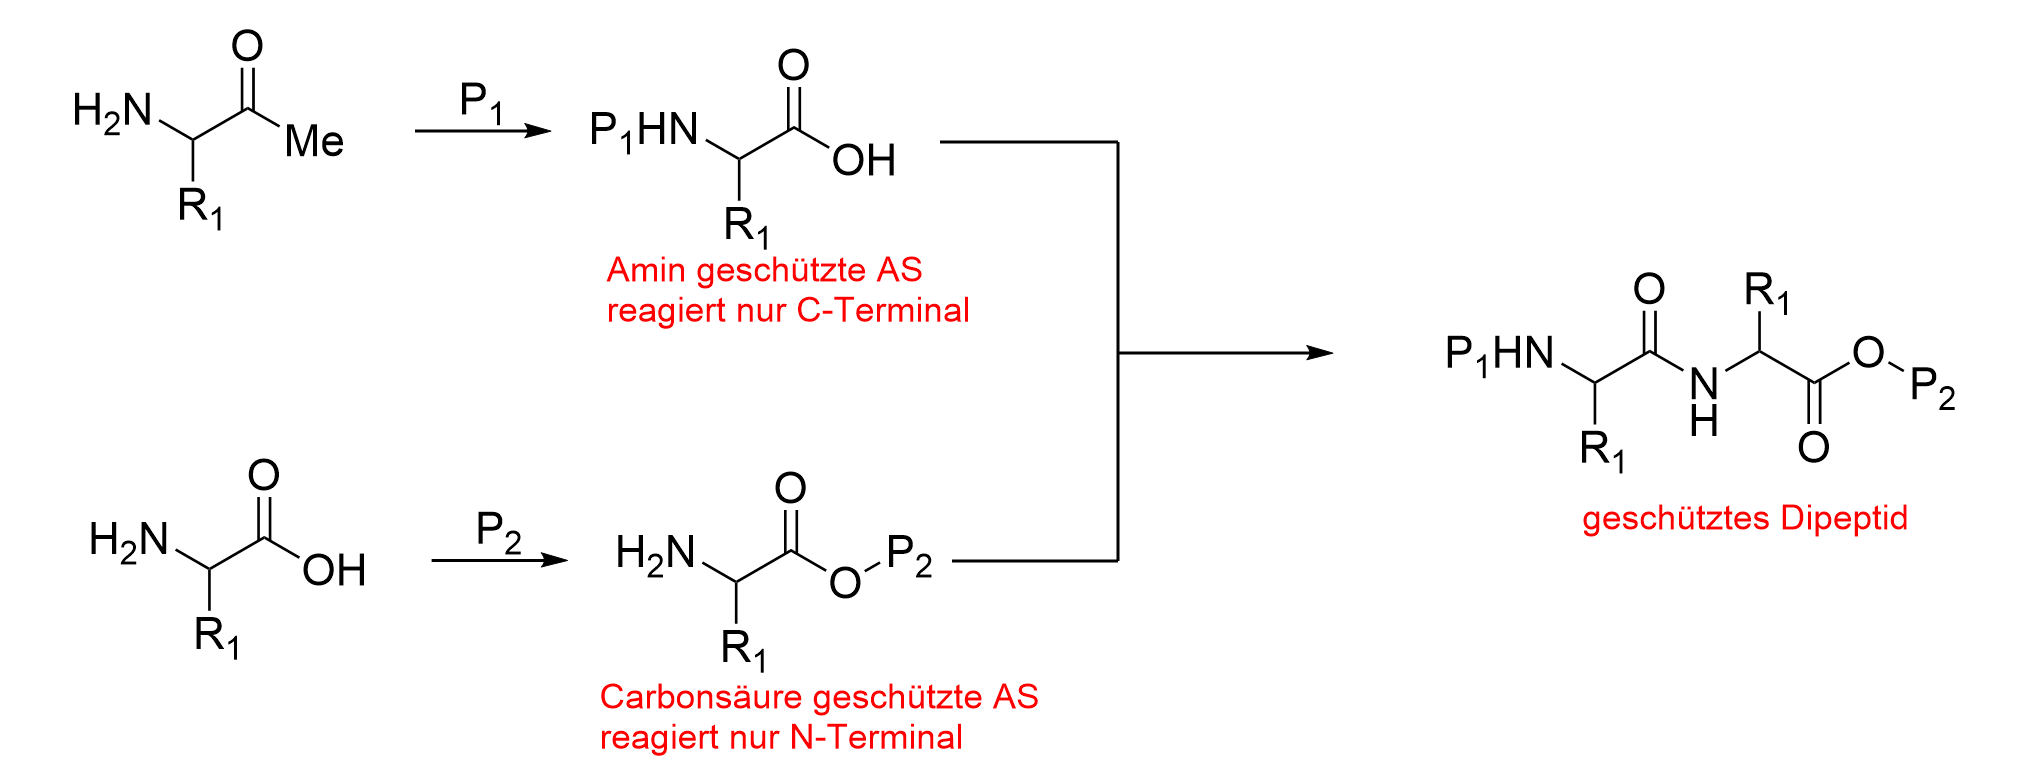
\includegraphics[width=1\linewidth]{Bilder/Peptid Synthese in Lösung.png}
\end{figure}

\subsubsection*{Mernfield-Festphasensynthese}
\begin{figure}[H]
	\centering
	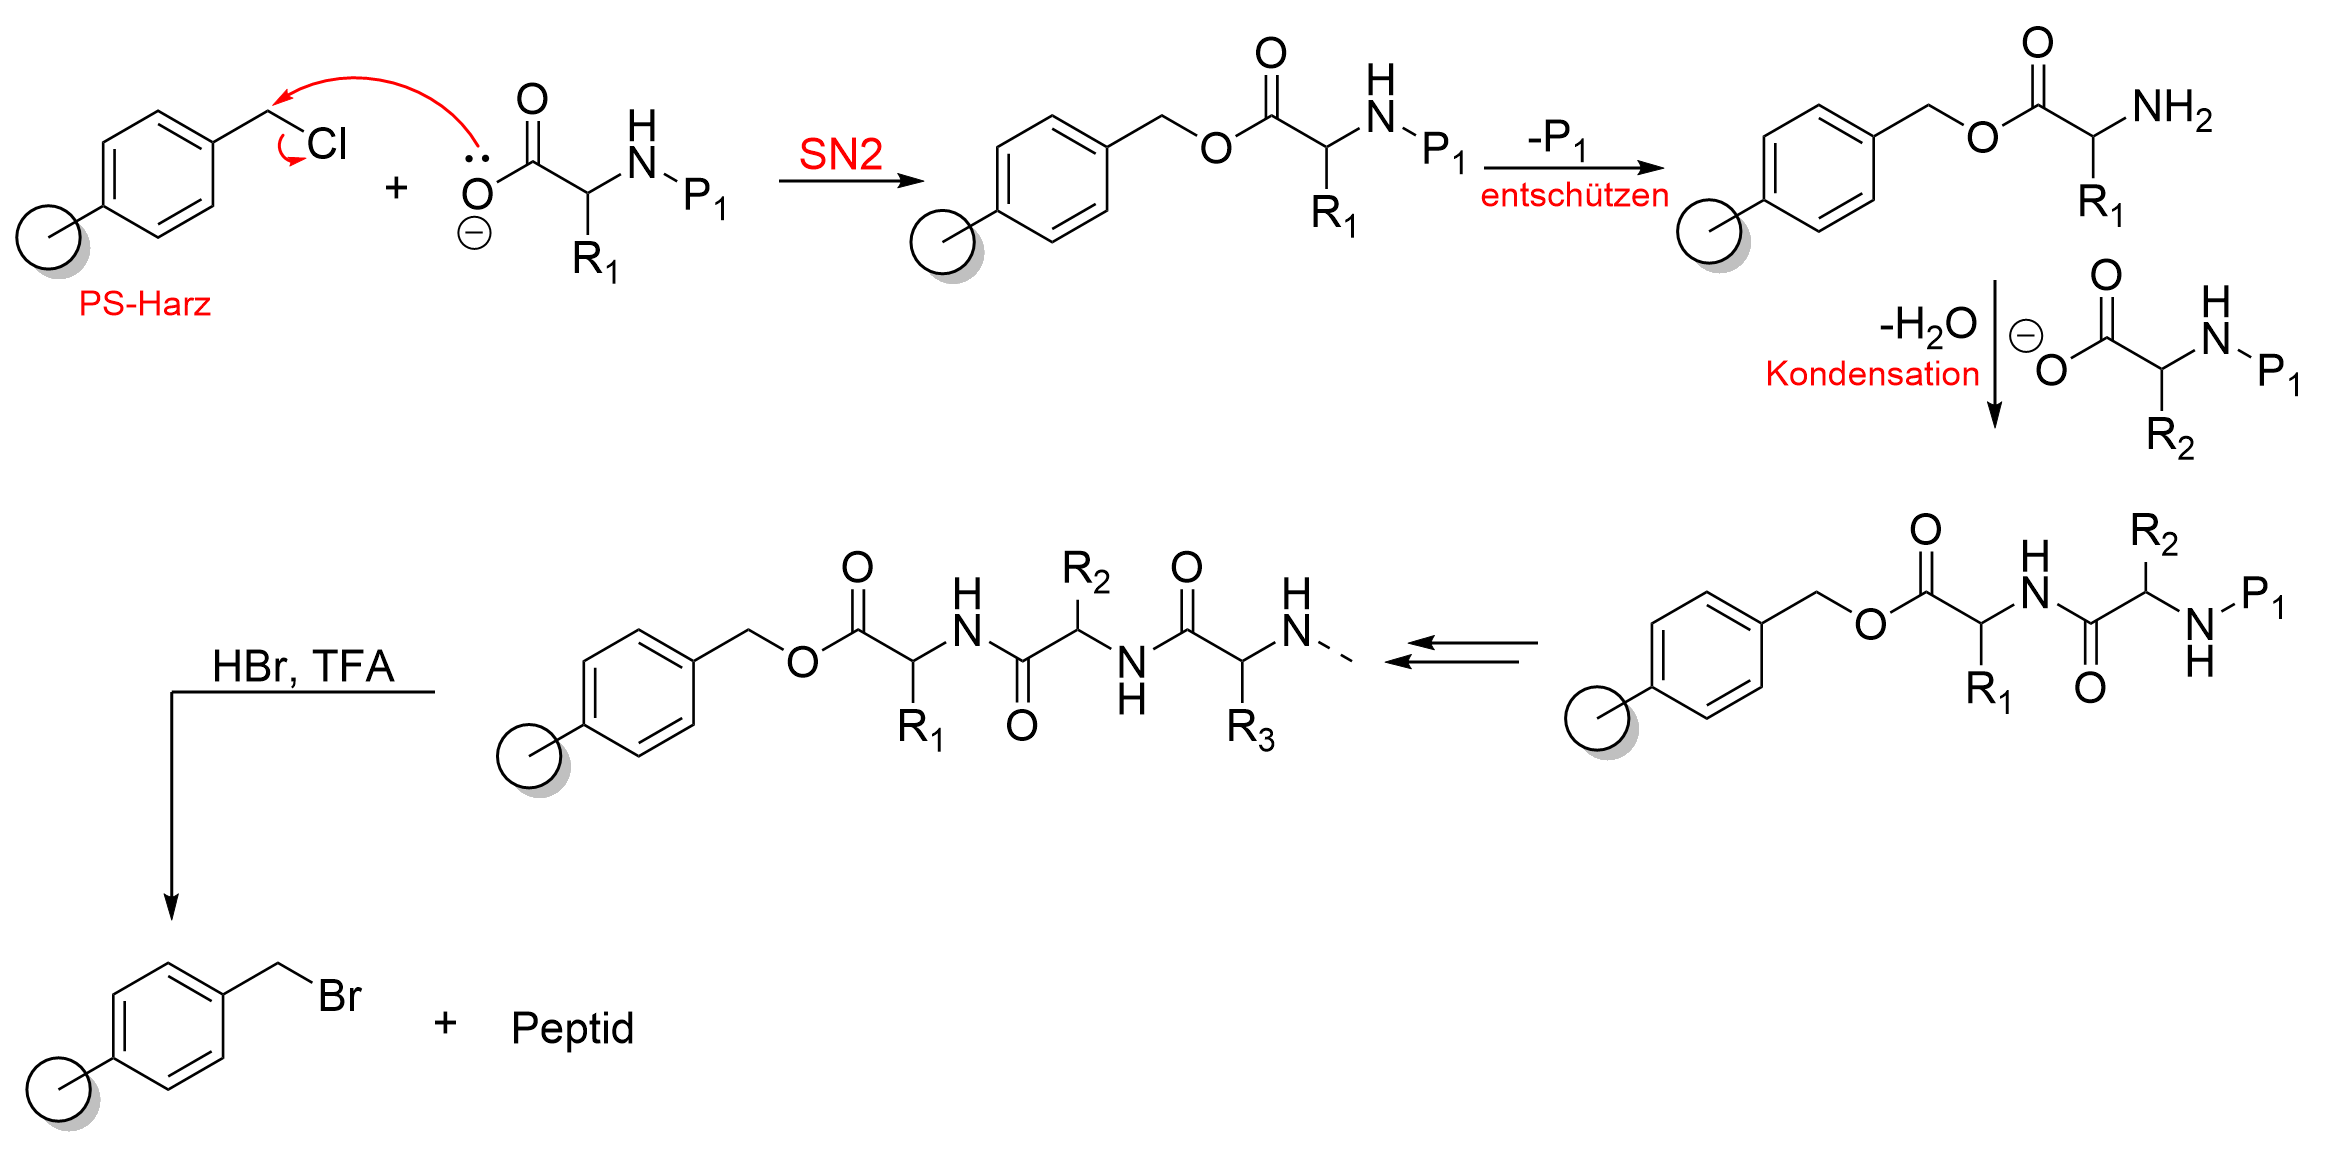
\includegraphics[width=1\linewidth]{Bilder/Mernfield-Festphasensynthese.png}
\end{figure}


\section{Kohlenhydrate}
Kohlenhydrate sind Polyhydroxyverbindungen mit Aldehyden/Ketofunktionen.
Ihre Summenformel ist \ce{C_n(H2O)_m}, daher kommt der Name Kohlen-Hydrat.
Diese Summenformel ist historisch geprägt und stimmt daher nicht immer.\\
Kohlenhydrate können eingeteilt werden in
\begin{itemize}
	\item Monosacharide: nur 1 Kohlenhydratbaustein
	\item Oligosacharide: $>10$ Kohlenhydratbausteine
\end{itemize}

\subsection{Monosacharide}
Monosacharide können entweder Ketone oder Aldehyde sein. Hierfür werden die Begriffe Aldosen und Ketosen verwendet.
\begin{figure}[H]
	\centering
	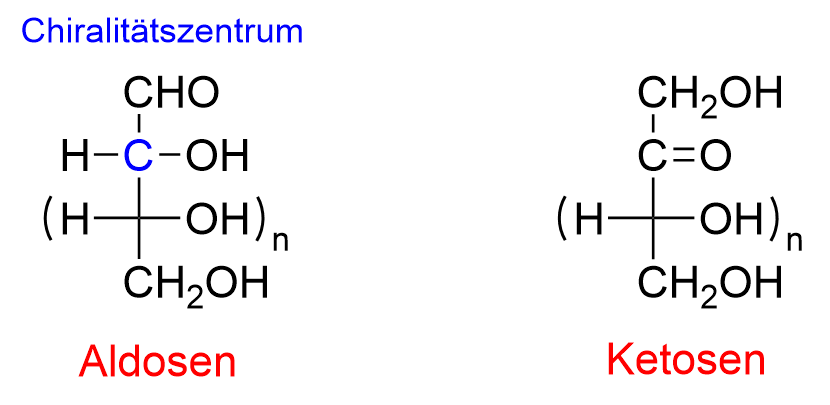
\includegraphics[width=0.6\linewidth]{Bilder/Ketose-Aldose.png}
\end{figure}
\noindent Die Begriffe Aldose und Ketose beschreiben nur ob es sich um ein Monosacharid mit Keton oder Aldehyd Funktion handelt. Die Kohlenstoffzahl eines Monosacharids lässt sich durch folgende Bezeichnungen beschreiben:
\begin{itemize}
	\item Triose: 3xC-Atome
	\item Tetrose: 4xC-Atome 
	\item Pentose: 5xC-Atome
	\item Hexose: 6xC-Atome
\end{itemize}
Diese beiden Bezeichnungen lassen sich kombinieren. Erst kommt die Unterscheidung Aldose Ketose mit den Präfixen Aldo- und Keto- und anschließend die Bezeichnung für die Anzahl der Kohlenstoffe. Ein Beispiel wäre Aldohexose für die Glucose oder Ketohexose für die Fructose. \\
\noindent Jedoch gibt es für die Monosacharide viele unterschiedliche Namen, darunter die meisten Trivialnamen.


\subsection{Physikalische Eigenschaften}
Zucker sind aufgrund der vielen OH-Gruppen sehr polar und sehr gut wasserlöslich. Wasserstoffbrücken stärken den Zusammenhalt im Kristall.

\subsection{Stereochemie der Monosacharide}
Der einfachste Grundkörper ist Glycerinaldehyd (Aldotriose).
Diese liegt sowohl als (S)(-)-Glycerinaldehyd und (R)(+)-Glycerinaldehyd vor. Da bei höheren Monosachariden die R/S Nomenklatur unübersichtlich wird, wird die D/L-Nomenklatur verwendet. Dort bezieht sich die D/L-Konfiguration bei Anwesenheit mehrerer Stereozentren immer auf das letzte asymmetrische C-Atom.
\begin{figure}[H]
	\centering
	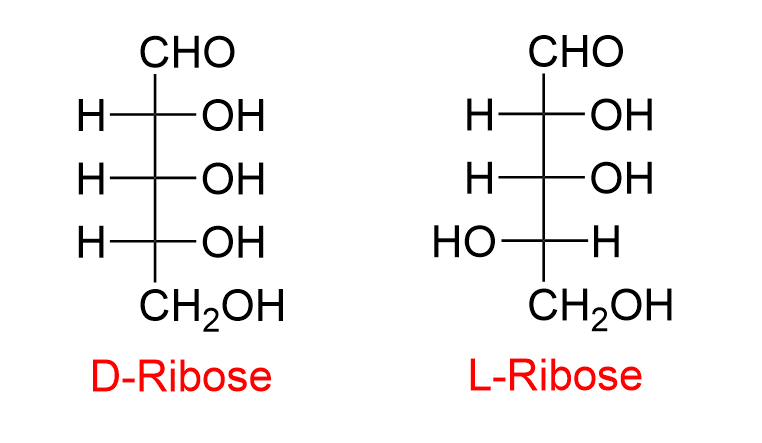
\includegraphics[width=0.6\linewidth]{Bilder/Stereochemie DL.png}
\end{figure}
\noindent Die Anzahl der Stereoisomere ergibt sich aus der Anzahl der Chiralitätszentren mit der Formel $2^n$. In der Natur sind D-Zucker wesentlich häufiger als L-Zucker. Epimere sind Diastereomere, die sich nur in der Konfiguration eines Stereozentrum unterscheiden.
\begin{figure}[H]
	\centering
	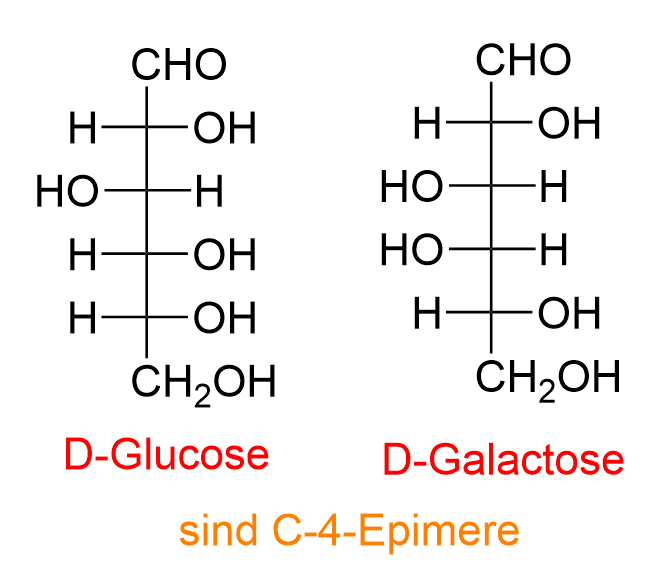
\includegraphics[width=0.5\linewidth]{Bilder/Epimere.png}
\end{figure}
\noindent Kohlenhydrate liegen überwiegend als cyclische Strukturen (Halbacetale) vor. Die offenkettige Form macht weniger als 0,5\% aus.
\begin{figure}[H]
	\centering
	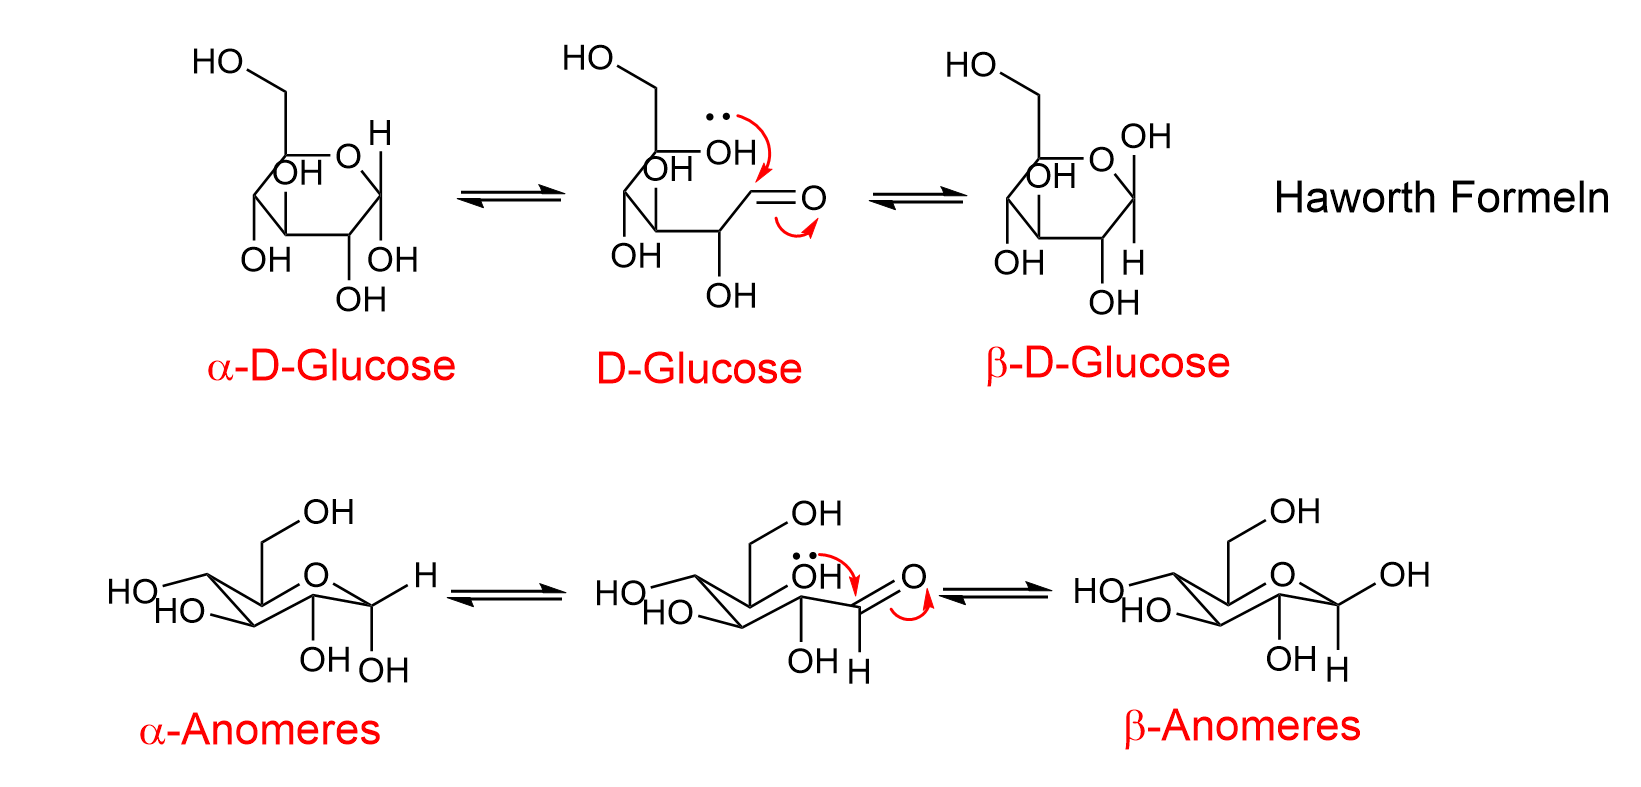
\includegraphics[width=1\linewidth]{Bilder/Cyclische Monosacharide.png}
\end{figure}
\noindent Anomere sind Diastereomere, die sich in der Konfiguration ihrer cyclischen Form an C1 bei Aldosen und C2 bei Ketosen unterscheiden (Mutarotation). Das Gleichgewicht der Anomere wird durch 1,3-Diaxiale Wechselwirkungen bestimmt.\\

\noindent Neben 6-Ring Halbacetalen können auch 5-Ring Halbacetale gebildet werden. 6-Ring Halbacetale werden als Pyranosen (abgeleitet von pyran) und 5-Ring Halbacetale als Furanosen (abgeleitet von Furan) bezeichnet. Die Mutarotation von Furanosen ist analog zu der oben gezeigten von D-Glucose Mutarotationen werden durch Säuren und Basen katalysiert.

\subsection{Darstellung}
\subsubsection{Photosynthese}
\begin{equation*}
	\ce{6CO2 + 6H2O ->[h\nu] 6O2 + C6H12O6 ->[\text{Glycosyltransferase}] \text{Cellulose, Stärke,...}}
\end{equation*}


\subsection{Reaktionen}
\subsubsection{Fehling-Probe}
\begin{figure}[H]
	\centering
	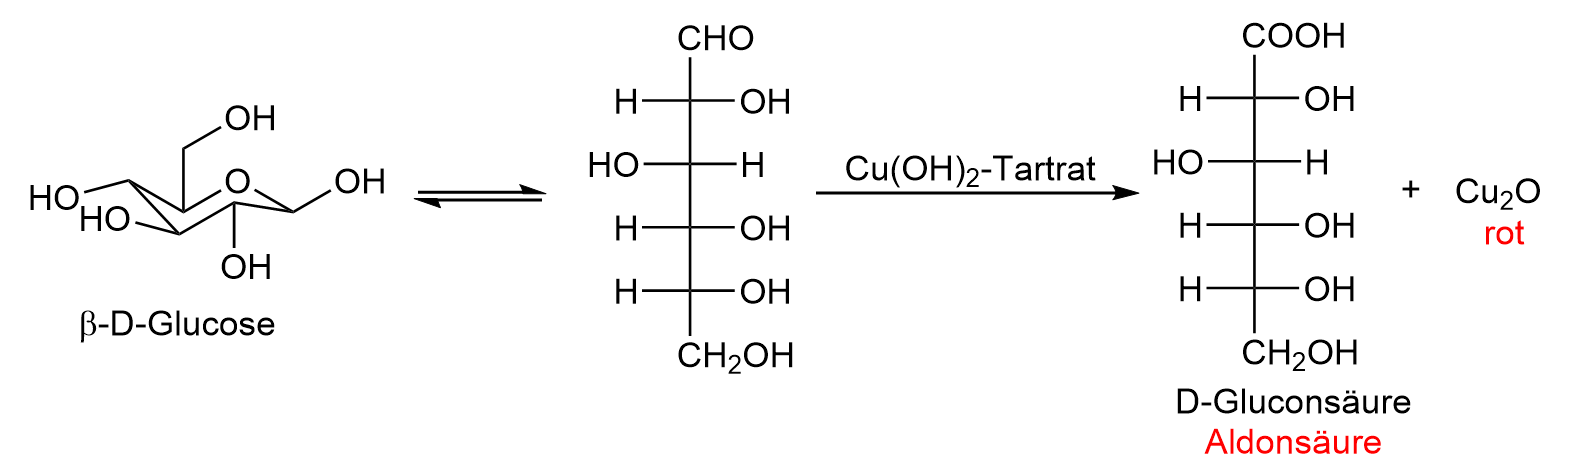
\includegraphics[width=0.9\linewidth]{Bilder/Fehling.png}
\end{figure}
Es werden nicht nur Aldosen positiv getestet sondern auch Ketosen. Der Grund hierfür ist die Tautomerisierung der Ketosen zu Aldosen über Keto-Enol-Tautomerie im alkalischen. Dies gilt sowohl für Fehling als auch für Tollens.

\subsubsection{Tollens-Probe}
Die Tollens Probe oxidiert analog zur Fehling Probe reduzierende Zucker. Bei der Tollens Probe wird Silber abgeschieden und es entsteht ein Silberspiegel. 

\subsubsection{Oxidation mit Brom}
Diese Reaktion ist spezifisch für Aldosen. Ketosen reagieren nicht mit Brom.
\begin{figure}[H]
	\centering
	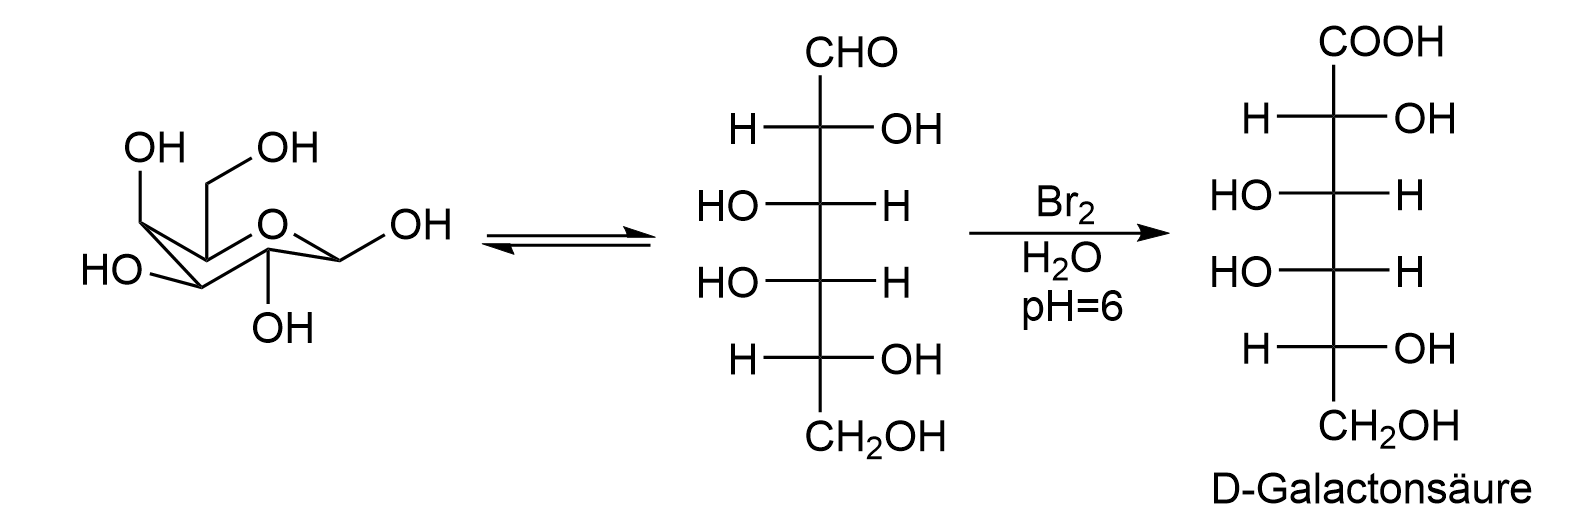
\includegraphics[width=0.8\linewidth]{Bilder/Oxidation von Aldosen.png}
\end{figure}

\subsubsection{Oxidation mit Salpetersäure}
\begin{figure}[H]
	\centering
	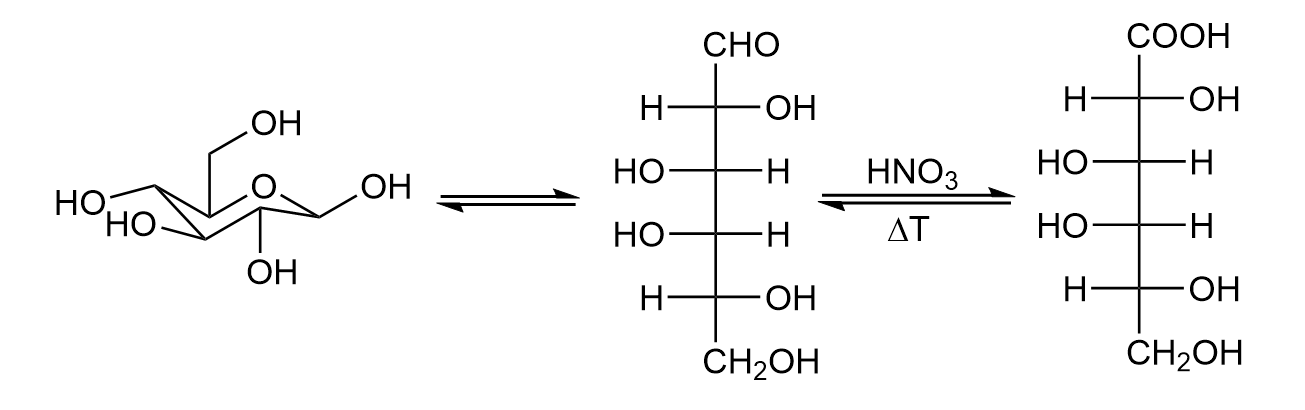
\includegraphics[width=0.8\linewidth]{Bilder/Oxidation von Aldosen mit HNO3.png}
\end{figure}

\subsubsection{Seliwanow Probe}
Die Seliwanow Probe dient der Unterscheidung von Aldosen und Ketosen.
\begin{figure}[H]
	\centering
	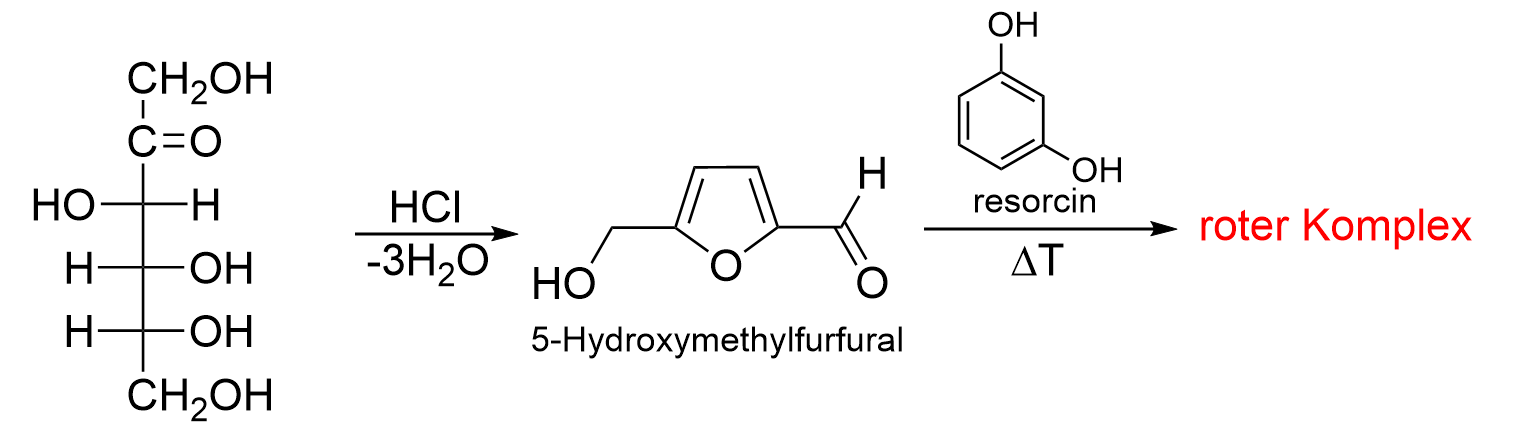
\includegraphics[width=0.85\linewidth]{Bilder/Seliwanow Probe.png}
\end{figure}
Die Reaktion funktioniert bevorzugt mit Hexosen.

\subsubsection{Reduktion mit \ce{NaBH4}}
\begin{figure}[H]
	\centering
	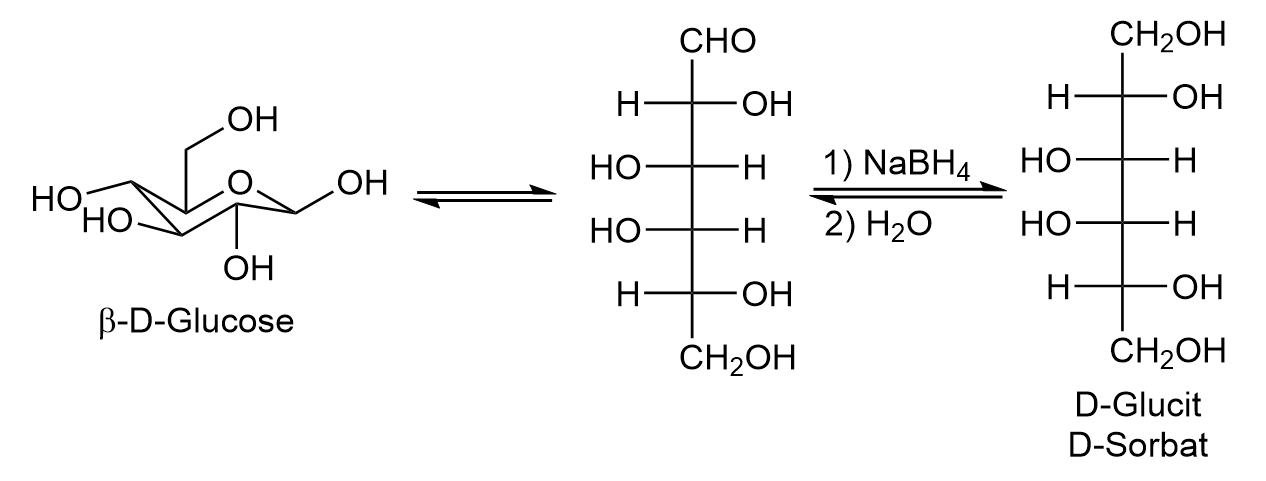
\includegraphics[width=0.8\linewidth]{Bilder/Reduktion von Aldosen.png}
\end{figure}

\subsubsection{Bisulfit Addition an Glucose}
Die Bisulfit Addition von Glucose liefert kein Bisulfit-Addukt. Dies ist ein Hinweis auf die Halbacetalform der Glucose.


\subsubsection{Maillard Reaktion}
\begin{figure}[H]
	\centering
	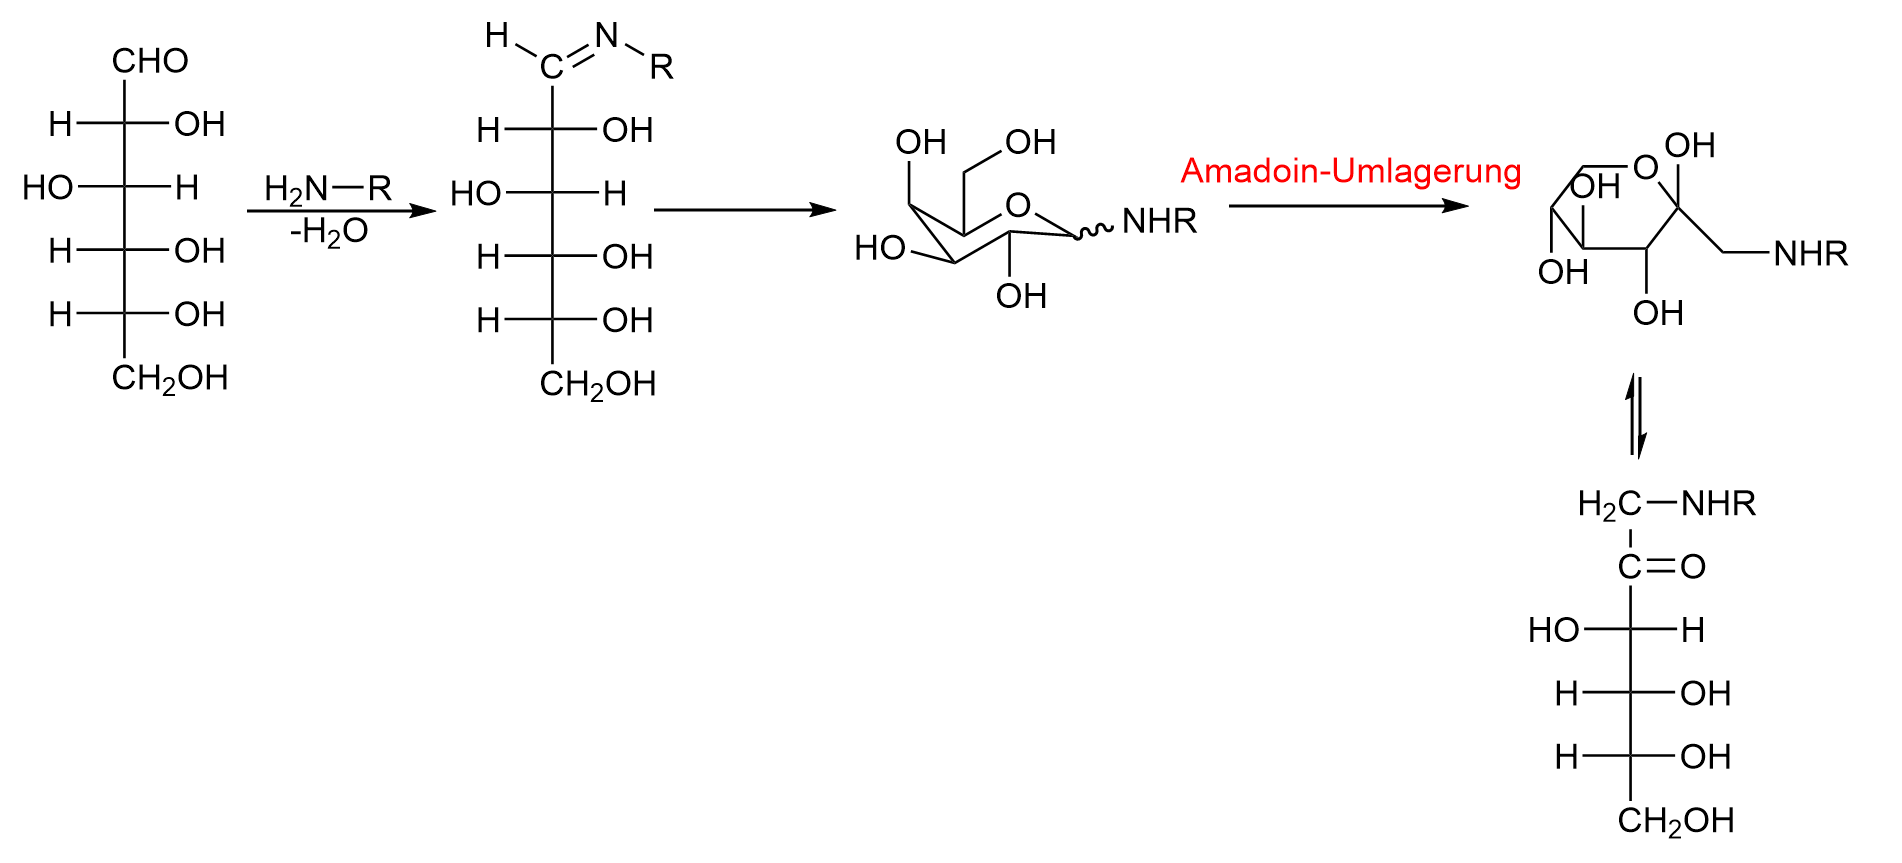
\includegraphics[width=0.9\linewidth]{Bilder/Maillard-Reaktion.png}
\end{figure}
Bei \ce{H2N-R} handelt es sich um die Amin-Funktion einer Aminosäure. Diese wird bei der Reaktion an die Aldose addiert.
Es bilden sich Stoffe, die für das Koch und Brataroma von tierischen oder pflanzlichen Lebensmitteln verantwortlich sind (nicht enzymatische Bräunung). Die Maillard-Reaktion ist aber auch medizinisch Relevant (Grauer Star, Trübung der Augen).


\subsubsection{Umwandlung von Monosachariden}
\subsubsection*{Aldose zu Ketose}
\begin{figure}[H]
	\centering
	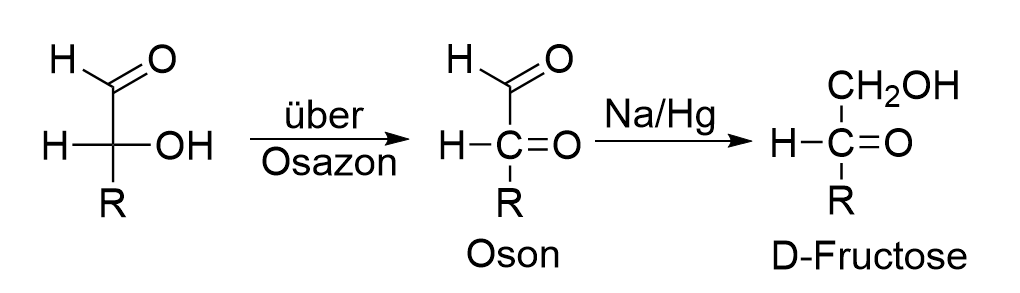
\includegraphics[width=0.7\linewidth]{Bilder/Aldose-Ketose Umwandlung.png}
\end{figure}

\subsubsection*{Basenkatalysierte Epimerisierung}
\begin{figure}[H]
	\centering
	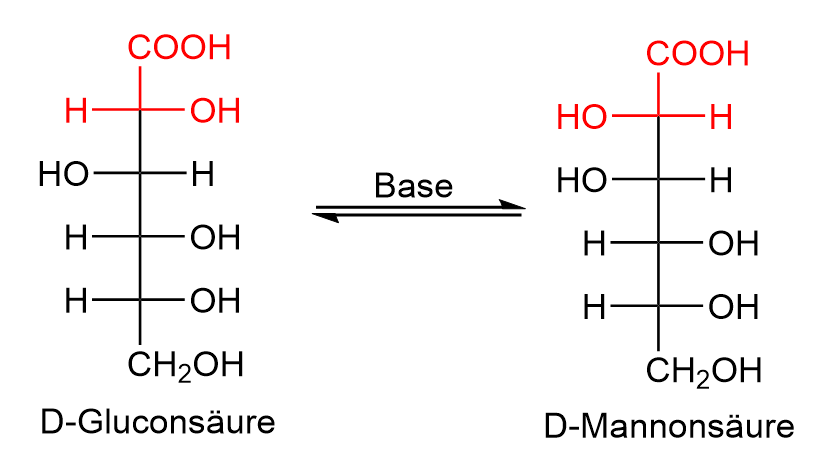
\includegraphics[width=0.7\linewidth]{Bilder/Basenkatalysierte Epimerisierung.png}
\end{figure}

\subsubsection{Kettenverlängerung: Kilian-Fischer}
\begin{figure}[H]
	\centering
	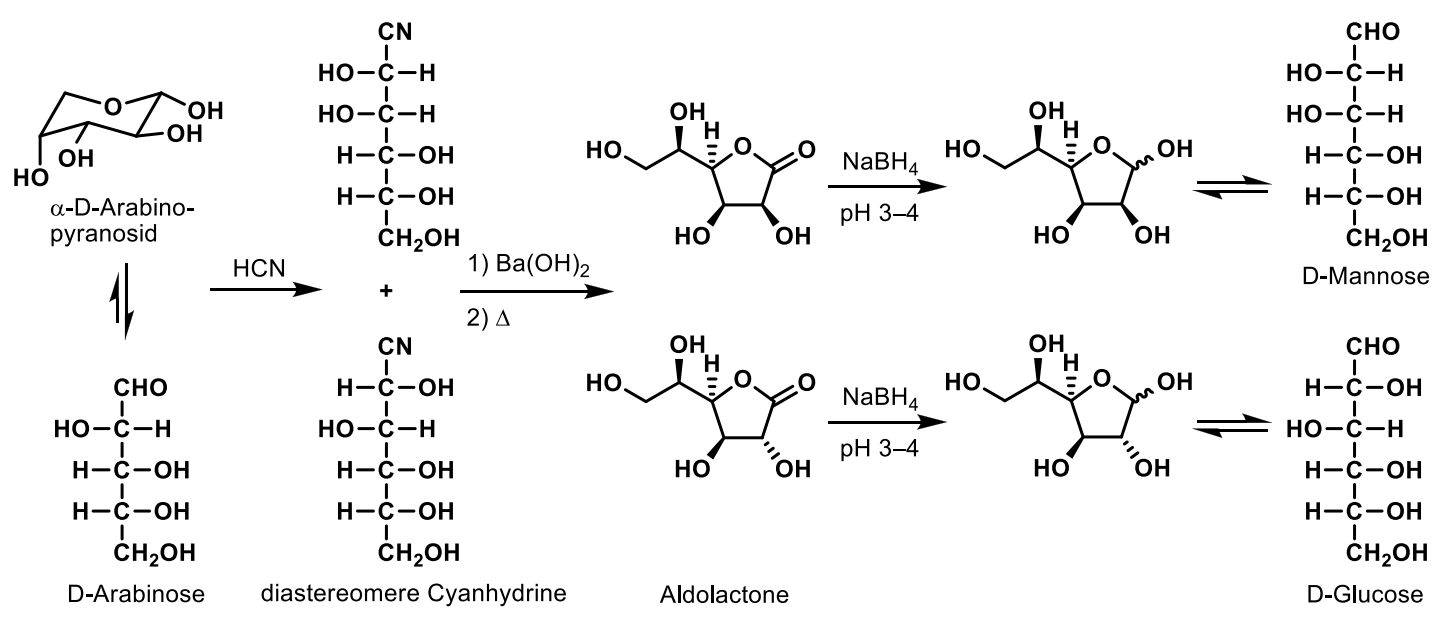
\includegraphics[width=1\linewidth]{Bilder/Kilian Fischer.png}
\end{figure}

\subsubsection{Kettenverkürzung}
\subsubsection*{Ruff Abbau}
\begin{figure}[H]
	\centering
	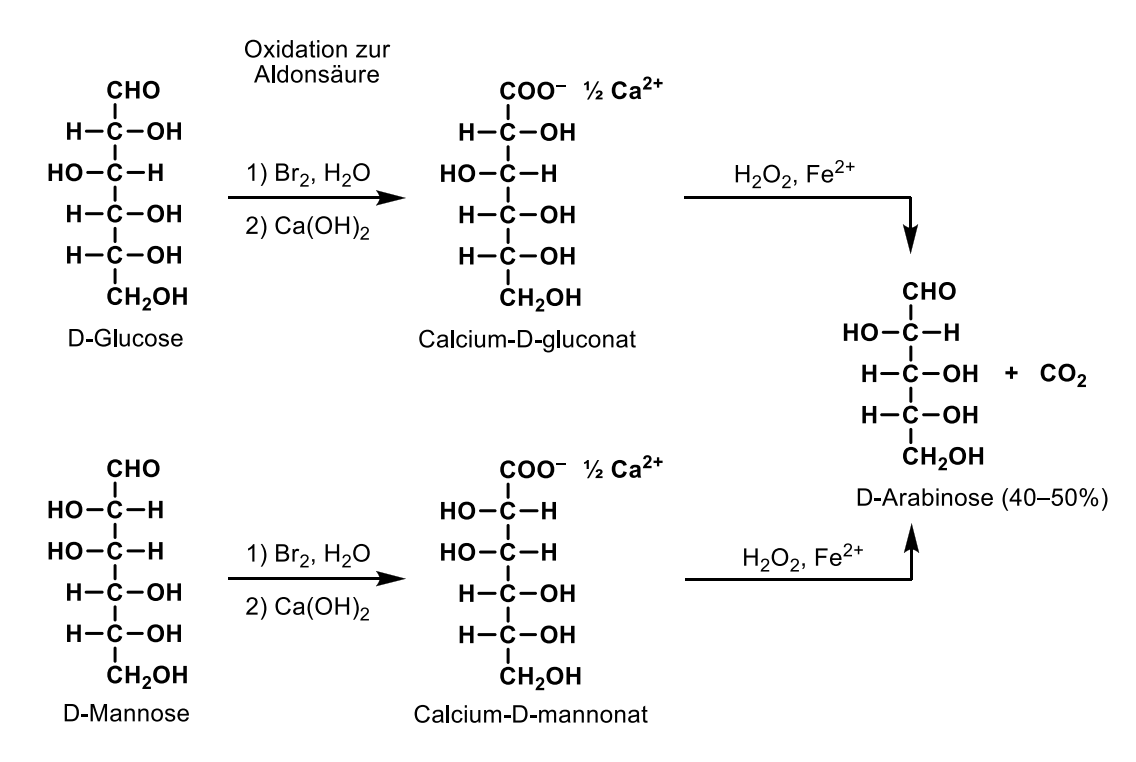
\includegraphics[width=1\linewidth]{Bilder/Ruff-Abbau.png}
\end{figure}

\subsubsection*{Wohl Abbau}
\begin{figure}[H]
	\centering
	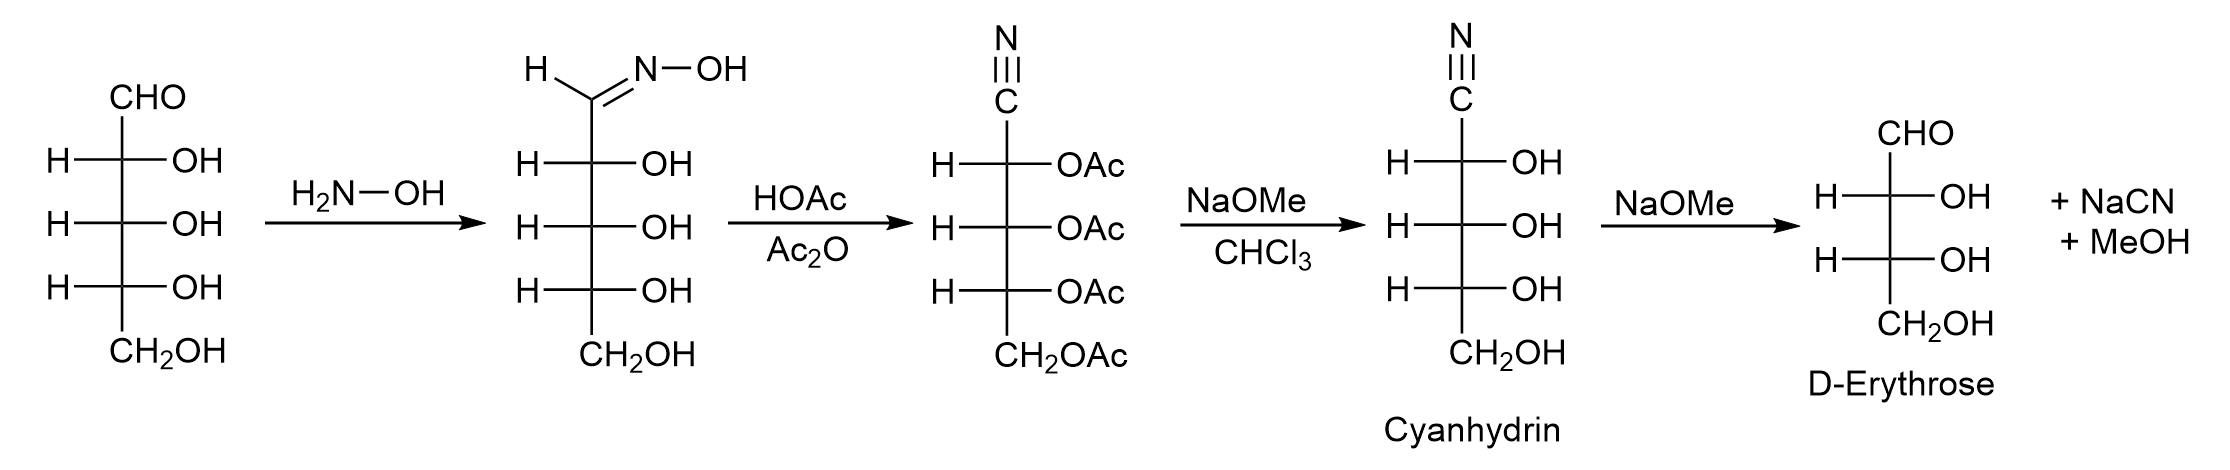
\includegraphics[width=1\linewidth]{Bilder/Wohl Abbau.png}
\end{figure}
Die Reaktion kann auf Pentosen, Hexosen angewandt werden.



\subsubsection{Glykosylierung}
Unter einer Glykolysierung versteht man die Anbindung eines Zuckers an nicht Zucker-Moleküle. Das Produkt heißt Glykosid bzw bei Proteinen Glykoprotein.
\begin{figure}[H]
	\centering
	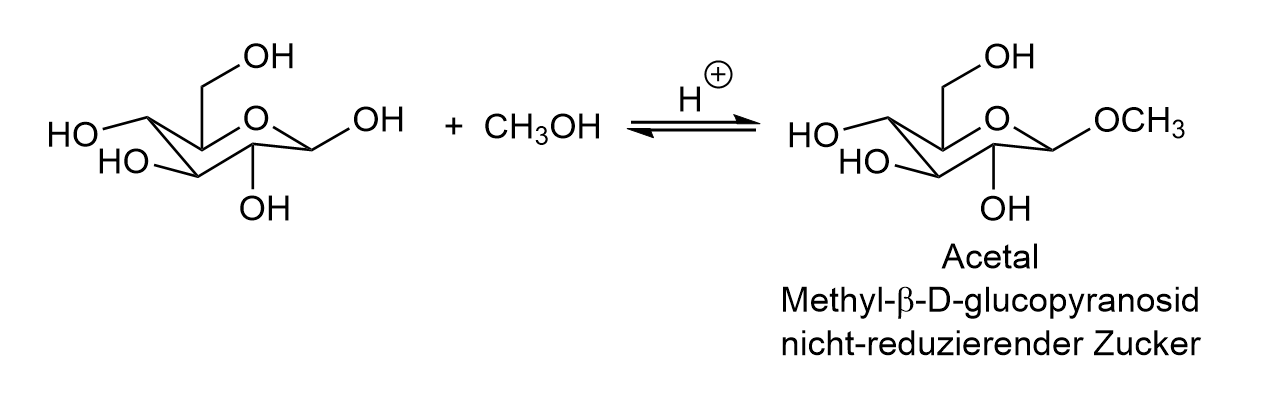
\includegraphics[width=0.9\linewidth]{Bilder/Glycosylierung.png}
\end{figure}
\noindent Nach dieser Glycolysierung fällt Fehling negativ aus, nach erhitzen im Sauren positiv. Glycoside spielen eine wichtige Rolle bei vielen Naturstoffen und bei Oligo- und Polysachariden.


\subsection{Disacharide}
\begin{figure}[H]
	\centering
	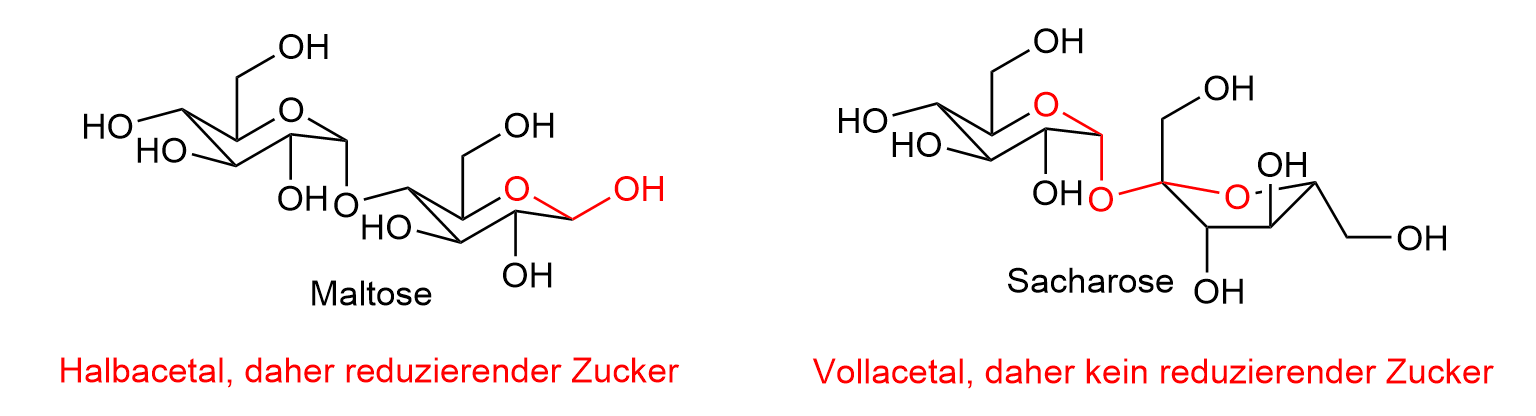
\includegraphics[width=0.9\linewidth]{Bilder/Disacharidew.png}
\end{figure}

\subsection{Polysacharide}
Polysacharide lassen sich in lineare (Cellulose, Amylose), verzweigte (Amylopektin, Glykogen) und cyclische Polysacharide (Cyclodextrin) unterteilen. 
\begin{figure}[H]
	\centering
	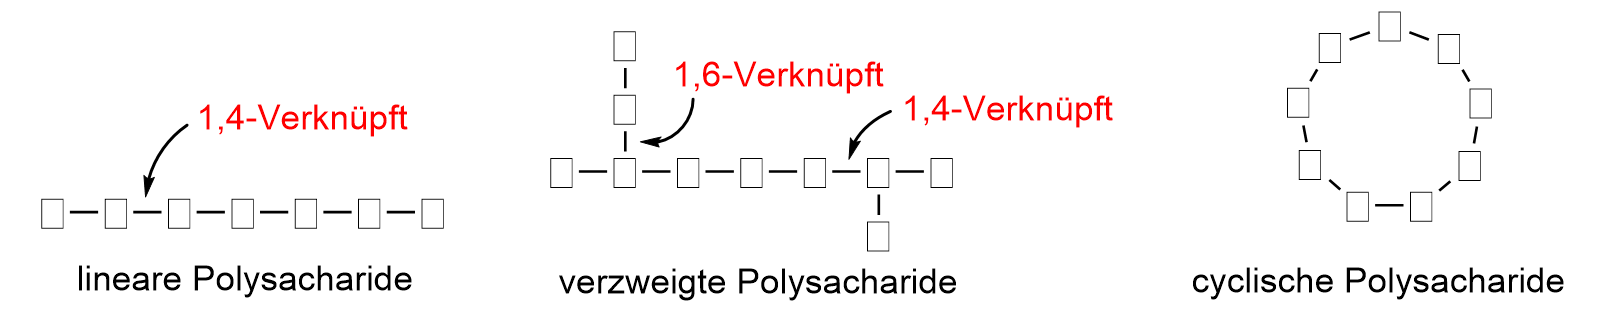
\includegraphics[width=1\linewidth]{Bilder/Polysacharide.png}
\end{figure}





\subsection{Süßstoffe}


\subsection{Funktionen von Kohlenhydraten}
\begin{itemize}
	\item Energiespeicher
	\item Stützfunktion
	\item Zell-Zell-Erkennung
	\item Signaltransduktion
	\item Speicherung und Stabilisierung von Sekundärmetaboliten
	\item Erhöhung der Wasserlöslichkeit durch Glycosylierung 
	\item Bestandteile von Cofaktoren
	\item Bestandteile der Nukleinsäuren (DNA, RNA)
\end{itemize}


\end{document}
